% =============================================================================
%  TPF -- IA aplicada a la Robótica
%  Resumen completo del trabajo, para uso propio: cómo funciona la
%  arquitectura, qué hace cada archivo, qué hace cada parámetro y de dónde
%  salió cada número. Estado al 2026-10-02 (demo completa andando en el piso,
%  con ultrasónico y buzzer).
%
%  Compilar (dos pasadas, por el índice):
%      pdflatex TPF_resumen.tex
%      pdflatex TPF_resumen.tex
%  o bien:  latexmk -pdf TPF_resumen.tex
%
%  El contenido está partido en secciones/*.tex; las imágenes en figuras/.
%  Las fuentes de cada dato son PLAN.md (§13, la bitácora), HARDWARE.md,
%  RUNBOOK.md y los comentarios de src/config.py.
% =============================================================================
\documentclass[aspectratio=169,9pt]{beamer}

\usetheme{metropolis}
\usepackage[T1]{fontenc}
\usepackage[utf8]{inputenc}
\usepackage[spanish,es-noquoting]{babel}
\usepackage{tikz}
\usetikzlibrary{positioning,arrows.meta,shapes.geometric,fit,backgrounds,calc,
                decorations.pathreplacing}
\usepackage{booktabs}
\usepackage{amsmath}
\usepackage{array}
\usepackage{xcolor}
\usepackage{graphicx}
% Sin ligaduras en la tipografía de máquina: si no, "--grabar" sale con un
% solo guión y ">>" como comillas angulares.
\usepackage{microtype}
\DisableLigatures{encoding = T1, family = tt*}

\graphicspath{{figuras/}}

% ------------------------------------------------------------------ Colores
% La misma paleta que la presentación de arquitectura y que las figuras del
% cuaderno de calibración: azul = rueda izquierda, naranja = rueda derecha.
\definecolor{azul}{HTML}{2A78D6}
\definecolor{naranja}{HTML}{EB6834}
\definecolor{gris}{HTML}{52514E}
\definecolor{grisclaro}{HTML}{898781}
\definecolor{critico}{HTML}{D03B3B}
\definecolor{verde}{HTML}{0CA30C}
\definecolor{ambar}{HTML}{FAB219}

\setbeamercolor{frametitle}{bg=azul}
\setbeamercolor{progress bar}{fg=naranja}
\setbeamercolor{alerted text}{fg=critico}
\setbeamertemplate{frame numbering}[fraction]
\metroset{block=fill}

% Densidad: son diapositivas de consulta, con más texto que una presentación
% para proyectar. Bloques compactos y márgenes angostos.
\setbeamerfont{block title}{size=\small}
\setbeamerfont{block body}{size=\small}
\setbeamerfont{itemize/enumerate body}{size=\small}
\setbeamerfont{itemize/enumerate subbody}{size=\footnotesize}
\setbeamersize{text margin left=6mm, text margin right=6mm}
\addtobeamertemplate{block begin}{\vspace{-0.25em}}{}
\addtobeamertemplate{block end}{}{\vspace{-0.55em}}
\addtobeamertemplate{block alerted begin}{\vspace{-0.25em}}{}
\addtobeamertemplate{block alerted end}{}{\vspace{-0.55em}}
\addtobeamertemplate{block example begin}{\vspace{-0.25em}}{}
\addtobeamertemplate{block example end}{}{\vspace{-0.55em}}
\setlength{\parskip}{0.25em}
\setlength{\tabcolsep}{4pt}

% ------------------------------------------------------------------ Atajos
\newcommand{\autornombre}{Federico Morán}
\newcommand{\listo}{\textcolor{verde}{$\blacksquare$}}
\newcommand{\curso}{\textcolor{ambar}{$\blacksquare$}}
\newcommand{\pend}{\textcolor{grisclaro}{$\square$}}
\newcommand{\hacia}{$\rightarrow$}
\newcommand{\grad}{\ensuremath{^\circ}}
\newcommand{\destaca}[1]{\textcolor{azul}{\textbf{#1}}}
\newcommand{\ojo}[1]{\textcolor{critico}{\textbf{#1}}}
% Código en línea: nombres de archivo, parámetros, comandos. \detokenize deja
% pasar los guiones bajos sin escaparlos. No puede llevar % ni # adentro.
\newcommand{\cod}[1]{\texttt{\detokenize{#1}}}
% Fila de una tabla de parámetros: nombre, valor, qué hace, de dónde sale.
\newcommand{\fila}[4]{\cod{#1} & #2 & #3 & #4 \\}
% Columnas de párrafo alineadas a la izquierda, sin justificar.
\newcolumntype{L}[1]{>{\raggedright\arraybackslash}p{#1}}

% ------------------------------------------------------------------ Portada
\title{Robot autónomo de aproximación y evasión basado en visión}
\subtitle{Resumen completo del trabajo: arquitectura, archivos, parámetros y
          todo lo que se midió hasta hoy}
\author{\autornombre}
\institute{TPF --- IA aplicada a la Robótica \\ Maestría en Inteligencia Artificial}
\date{Estado al 2 de octubre de 2026}

\begin{document}

\maketitle

% =============================================================================
%  1. Panorama: qué es, qué hace hoy, qué quedó afuera
% =============================================================================

\begin{frame}{Para qué es este documento}
  \begin{block}{Objetivo}
    Tener en un solo lugar \destaca{todo el trabajo}: qué hace el robot, cómo
    está armado, qué hace cada archivo y cada parámetro, y \destaca{de dónde
    salió cada número}. Es un resumen para mí, no para proyectar: tiene más
    texto que una presentación normal.
  \end{block}

  \vspace{0.3em}
  Cómo está organizado:
  \begin{enumerate}
    \item \textbf{Panorama} --- qué hace hoy y qué quedó afuera.
    \item \textbf{Hardware} y \textbf{arquitectura} --- las piezas y cómo se hablan.
    \item \textbf{Archivo por archivo} --- el código del Pi y el firmware del ESP32.
    \item \textbf{Comportamiento} --- la máquina de estados y la ley de control.
    \item \textbf{Parámetro por parámetro} --- qué hace cada uno y por qué vale lo que vale.
    \item \textbf{Historia} --- las 15 jornadas, lo que se midió y lo que falló.
    \item \textbf{Operación y pendientes} --- cómo se usa y qué falta.
  \end{enumerate}

  \vspace{0.2em}
  {\footnotesize Fuentes: \cod{PLAN.md} (el plan y la bitácora), \cod{HARDWARE.md},
  \cod{RUNBOOK.md}, los comentarios de \cod{src/config.py} y los registros de
  \cod{logs/}. Si algo de acá no coincide con esos archivos, mandan ellos.}
\end{frame}

\begin{frame}{Índice}
  \setbeamertemplate{section in toc}[sections numbered]
  \begin{columns}[T,onlytextwidth]
    \begin{column}{0.48\textwidth}
      {\footnotesize\tableofcontents[sections={1-8},hideallsubsections]}
    \end{column}
    \begin{column}{0.48\textwidth}
      {\footnotesize\tableofcontents[sections={9-15},hideallsubsections]}
    \end{column}
  \end{columns}
\end{frame}

% =============================================================================
\section{Panorama}
% =============================================================================

\begin{frame}{El objetivo, en una frase}
  \begin{alertblock}{}
    \centering\large
    Un robot que \textbf{recorre una sala}, \textbf{reconoce dos objetos con la
    cámara} y \textbf{se comporta distinto con cada uno}: se acerca a uno y huye
    del otro.
  \end{alertblock}

  \vspace{0.6em}
  \begin{columns}[T]
    \begin{column}{0.48\textwidth}
      \begin{block}{Objetivo: el oso (\cod{teddy bear})}
        Un oso \textbf{impreso en una hoja A4} ($\sim$20 cm). El robot lo busca,
        se le acerca corrigiendo el rumbo con la cámara y frena a $\sim$30 cm.
      \end{block}
    \end{column}
    \begin{column}{0.48\textwidth}
      \begin{block}{Amenaza: la mochila (\cod{backpack})}
        Una mochila real. El robot retrocede, gira media vuelta y se aleja.
        Tiene \textbf{prioridad incondicional} sobre todo lo demás.
      \end{block}
    \end{column}
  \end{columns}

  \vspace{0.6em}
  \small
  Todo corre \textbf{a bordo}: una Raspberry Pi 5 con una red neuronal
  (YOLOv8n) decide, y un ESP32 mueve los motores. No hay PC externa, ni
  teleoperación, ni nube. La notebook sólo sirve para lanzar la corrida por SSH
  y mirar lo que pasa.
\end{frame}

\begin{frame}{Qué hace el robot hoy (medido en el piso el 1 y el 2 de octubre)}
  \relax{\footnotesize
  \begin{tabular}{L{2.4cm}L{8.3cm}L{3.0cm}}
    \toprule
    \textbf{Qué ve} & \textbf{Qué hace} & \textbf{Estado} \\
    \midrule
    Nada &
      Mira quieto $\sim$0,6 s, gira un paso de $\sim$18\grad{} y repite. Una
      vuelta entera tarda $\sim$17 s; después avanza $\sim$18 cm para cambiar el
      punto de vista y vuelve a empezar. &
      \cod{BUSCAR} \\[2pt]
    El oso &
      Se queda quieto hasta confirmarlo (3 frames, $\sim$0,3 s), se acerca
      centrándolo, frena a $\sim$30 cm y da un pitido largo. Si lo pierde, lo
      busca hacia el lado donde lo vio por última vez. &
      \cod{APROXIMAR} \hacia{} \cod{ENCONTRADO} \\[2pt]
    La mochila &
      Se queda quieto hasta confirmarla y, con la alarma sonando, retrocede
      $\sim$30 cm girando, sigue girando hasta darle la espalda y avanza
      $\sim$65 cm. Después vuelve a buscar. &
      \cod{HUIR} \\[2pt]
    Algo a menos de 30 cm adelante &
      Cuando va a avanzar sin el oso a la vista (huyendo o buscando), no
      avanza: gira en el lugar hasta tener el camino libre. &
      \cod{HUIR} o \cod{BUSCAR} \\[2pt]
    Oso y mochila &
      Huye: la amenaza gana siempre, incluso estando detenido frente al oso. &
      \cod{HUIR} \\
    \bottomrule
  \end{tabular}}

  \vspace{0.6em}
  \begin{columns}[T,onlytextwidth]
    \begin{column}{0.485\textwidth}
      \begin{block}{Lo que se probó}
        {\footnotesize Dieciséis corridas con motores en dos días: diez el 1
        de octubre y seis el 2, ya con el ultrasónico y el buzzer. Hay dos
        videos vistos desde el robot en \cod{media/}.}
      \end{block}
    \end{column}
    \begin{column}{0.485\textwidth}
      \begin{alertblock}{Lo que no se midió todavía}
        {\footnotesize Las 10 corridas por escenario que piden las métricas, y
        la autonomía del cargador. Los porcentajes de éxito no existen aún.}
      \end{alertblock}
    \end{column}
  \end{columns}
\end{frame}

\begin{frame}{Los números del sistema, de un vistazo}
  \relax{\footnotesize
  \begin{columns}[T,onlytextwidth]
    \begin{column}{0.49\textwidth}
      \begin{tabular}{L{3.9cm}L{2.9cm}}
        \toprule
        \textbf{Percepción} & \\
        \midrule
        Modelo & YOLOv8n (COCO) \\
        Tamaño de inferencia & 320 px \\
        FPS del lazo completo & $\sim$10,6 ($\sim$9,9 grabando) \\
        Inferencia por frame & $\sim$88 ms \\
        Edad del frame al decidir & $\sim$150 ms \\
        Alcance con el oso A4 & $\sim$1,3 m \\
        Campo visual horizontal & $\sim$52\grad \\
        Confirmar / perder & 3 / 5 frames \\
        \bottomrule
      \end{tabular}

      \vspace{0.5em}
      \begin{tabular}{L{3.9cm}L{2.9cm}}
        \toprule
        \textbf{Seguridad} & \\
        \midrule
        Vigencia del comando (Pi) & 0,40 s \\
        Watchdog (ESP32) & 500 ms \\
        Ultrasónico: esquivar / llegar & 30 / 20 cm \\
        Corte de emergencia & conector de 12 V \\
        \bottomrule
      \end{tabular}
    \end{column}
    \begin{column}{0.49\textwidth}
      \begin{tabular}{L{3.9cm}L{2.9cm}}
        \toprule
        \textbf{Movimiento} & \\
        \midrule
        Rango de velocidad & 0,091 a 0,380 m/s \\
        Velocidad máx. usada & 0,25 m/s \\
        Giro buscando & pasos de $\sim$18\grad \\
        Giro en régimen & 124 a 165\grad/s \\
        Distancia de frenado & $\sim$30 cm del oso \\
        Asimetría de los motores & 2,11 veces \\
        Trocha (regla / efectiva) & 21,5 / 18 cm \\
        Rueda & 60 mm de diámetro \\
        \bottomrule
      \end{tabular}

      \vspace{0.5em}
      \begin{tabular}{L{3.9cm}L{2.9cm}}
        \toprule
        \textbf{Verificación} & \\
        \midrule
        Verificaciones sin hardware & 79 \\
        Corridas registradas & CSV + JSON c/u \\
        \bottomrule
      \end{tabular}
    \end{column}
  \end{columns}}
\end{frame}

\begin{frame}{Qué entra en esta versión y qué quedó afuera}
  \begin{columns}[T,onlytextwidth]
    \begin{column}{0.485\textwidth}
      \begin{exampleblock}{Adentro, y funcionando}
        \begin{itemize}
          \item Detección con YOLOv8n a bordo, a $\sim$11 FPS.
          \item Máquina de estados con arbitraje: buscar, aproximar,
                encontrado, huir.
          \item Control proporcional sobre la imagen.
          \item ESP32 con protocolo serie, compensación de zona muerta por
                rueda y watchdog.
          \item Alimentación portátil con dos fuentes separadas.
          \item \textbf{Ultrasónico} al frente: no avanza contra lo que
                tenga a menos de 30 cm. \textbf{Buzzer}: alarma y llegada.
          \item Registro de cada corrida y análisis automático.
          \item 79 verificaciones del comportamiento sin hardware.
        \end{itemize}
      \end{exampleblock}
    \end{column}
    \begin{column}{0.485\textwidth}
      \begin{alertblock}{Afuera: segunda versión}
        \begin{itemize}
          \item \textbf{Sensores atrás y a los costados}: el robot
                \ojo{retrocede y gira a ciegas}, y una pared muy de costado no
                la ve.
          \item \textbf{Encoders}: sin odometría ni lazo de velocidad.
          \item \textbf{Frenar a 10 cm}: a esa distancia el oso no entra en el
                cuadro; haría falta un avance final a ciegas.
          \item \textbf{Cámara CSI} (Arducam): nunca fue vista por el Pi 5; se
                reemplazó por una webcam USB.
        \end{itemize}
      \end{alertblock}
    \end{column}
  \end{columns}

  \vspace{0.5em}
  {\footnotesize El ultrasónico y el buzzer habían quedado afuera el
  2026-10-01, por falta de tiempo, y entraron al día siguiente (sección ``El 2
  de octubre'').}
\end{frame}

\begin{frame}{Cómo se cubren los requisitos del módulo}
  \relax{\footnotesize
  \begin{tabular}{L{4.2cm}L{9.6cm}}
    \toprule
    \textbf{Requisito} & \textbf{Cómo se cubre} \\
    \midrule
    Aplicación de IA &
      Red convolucional de detección de objetos (YOLOv8n, preentrenada en COCO)
      haciendo inferencia en tiempo real sobre hardware embebido. \\[2pt]
    Vehículo autónomo no tripulado &
      Robot terrestre de tracción diferencial, con la decisión 100 \% a bordo. \\[2pt]
    Percepción \hacia{} decisión \hacia{} actuación &
      La cadena completa cerrada en el robot físico: cámara, red, máquina de
      estados, ley de control, enlace serie, motores. \\[2pt]
    Toma de decisiones &
      Máquina de estados con arbitraje explícito de conflictos: huir tiene
      prioridad sobre aproximarse. \\[2pt]
    Fusión de sensores &
      Cámara y ultrasónico. La cámara dice qué hacer y hacia dónde; el
      ultrasónico impide avanzar contra un obstáculo y puede dar por alcanzado
      el objetivo. Entró el 2026-10-02. \\
    \bottomrule
  \end{tabular}}

  \vspace{0.6em}
  \begin{block}{Lo que el trabajo demuestra}
    {\small Integrar \textbf{percepción con IA} en un \textbf{lazo de control
    físico} que corre en \textbf{tiempo real} sobre \textbf{hardware real}. La
    mitad de lo interesante salió de la última parte: motores con zonas
    muertas y asimetrías, imágenes que se rompen, baterías que no sostienen
    los 5 V.}
  \end{block}
\end{frame}

\begin{frame}{Las seis decisiones de diseño (1 de 2)}
  \relax{\small
  \begin{block}{D1 --- Un solo microcontrolador de bajo nivel: ESP32}
    Se descartó usar ESP32 y PSoC5LP a la vez: dos firmwares, dos protocolos y
    dos cadenas de herramientas duplican la superficie de fallas sin sumar
    nada. Se programa con PlatformIO, en estilo C.
  \end{block}
  \begin{block}{D2 --- Modelo preentrenado en COCO, sin entrenamiento propio}
    El ciclo captura \hacia{} etiquetado \hacia{} entrenamiento agregaba
    riesgo de cronograma sin ser el aporte del trabajo, que es \textbf{integrar
    la inferencia en un lazo de control físico}. Se compensa con más
    profundidad en control, arbitraje y medición.
  \end{block}
  \begin{block}{D3 --- Clases por nombre: \cod{teddy bear} y \cod{backpack}}
    Objetos medianos, compactos y de buen contraste. Las clases se declaran
    \textbf{por nombre} y se resuelven contra \cod{model.names}: si cambia el
    modelo, falla al arrancar en vez de detectar otra cosa en silencio.
    \ojo{En el piso apareció un matiz:} la mochila real es \cod{suitcase} para
    el modelo (ver la sección de la jornada final).
  \end{block}}
\end{frame}

\begin{frame}{Las seis decisiones de diseño (2 de 2)}
  \relax{\small
  \begin{block}{D4 --- Huir tiene prioridad sobre aproximar}
    Ante las dos clases a la vez, gana la conducta de seguridad. Es la regla
    clásica de la robótica de comportamientos: los de preservación subsumen a
    los de objetivo.
  \end{block}
  \begin{block}{D5 --- Encoders como extensión, no como núcleo}
    El sistema tiene que andar en lazo abierto (PWM directo, calibrado por
    rueda). Un PID sobre una planta descompensada arranca peor, así que la
    calibración había que hacerla igual. Los encoders quedaron sin cablear.
  \end{block}
  \begin{block}{D6 --- Confirmación temporal de las detecciones}
    Una detección aislada no cambia el estado: hacen falta \textbf{3 frames
    seguidos} para confirmar una clase y \textbf{5 sin verla} para darla por
    perdida. Evita que un falso positivo dispare una maniobra.
  \end{block}}

  \vspace{0.2em}
  {\footnotesize Y dos decisiones de arquitectura que salieron al implementar:
  la compensación de zona muerta vive \textbf{en el ESP32} y no en el Pi, y
  las capas que \emph{deciden} no tocan hardware (ver ``Arquitectura'').}
\end{frame}

% =============================================================================
\section{Hardware}
% =============================================================================

\begin{frame}{Inventario: qué hay arriba del chasis}
  \relax{\footnotesize
  \begin{tabular}{L{2.9cm}L{5.4cm}L{5.5cm}}
    \toprule
    \textbf{Componente} & \textbf{Detalle} & \textbf{Rol} \\
    \midrule
    Raspberry Pi 5 & 8 GB de RAM, sin monitor (\emph{headless}) &
      Alto nivel: cámara, red neuronal, máquina de estados, ley de control \\[1pt]
    ESP32 & DevKit con puente USB CP2102 &
      Bajo nivel: PWM de los motores, protocolo serie, watchdog \\[1pt]
    Driver L298N & Módulo comercial, puente H doble &
      Etapa de potencia de los dos motores \\[1pt]
    Motores (2) & GM25-370, 12 V, ``350 rpm'', con reductora &
      Tracción diferencial. \ojo{Las dos unidades no son iguales} \\[1pt]
    Chasis 2WD & Dos ruedas de 60 mm y una rueda loca &
      Locomoción \\[1pt]
    Cámara & Webcam USB Microsoft LifeCam Studio, 640$\times$480 en MJPG &
      Dice qué hay y hacia dónde \\[1pt]
    Ultrasónico & Parallax PING))), tres pines, al frente &
      Distancia a lo que tenga adelante. Desde el 2/10 \\[1pt]
    Buzzer & Activo, de dos patas &
      Alarma al huir y aviso al llegar. Desde el 2/10 \\[1pt]
    Cargador portátil & 20 000 mAh, 5 V / 3 A, por USB-A &
      Alimenta el Pi (y por sus USB, la webcam y el ESP32) \\[1pt]
    UPS & 10 000 mAh, salida de 12 V &
      Alimenta \textbf{sólo} el L298. Es el corte de emergencia \\[1pt]
    \textcolor{grisclaro}{Encoders Hall} & \textcolor{grisclaro}{uno por motor, sin cablear} &
      \textcolor{grisclaro}{Segunda versión} \\
    \bottomrule
  \end{tabular}}

  \vspace{0.4em}
  {\footnotesize El oso es una \textbf{impresión en hoja A4} ($\sim$20 cm de
  ancho) y la mochila es una mochila real, negra. Los dos son parte del
  sistema: los números de la calibración valen para \emph{esos} objetos.}
\end{frame}

\begin{frame}{El robot, en el banco (agosto de 2026; el terminado está en ``El 2 de octubre'')}
  \begin{columns}[c,onlytextwidth]
    \begin{column}{0.27\textwidth}
      \centering
      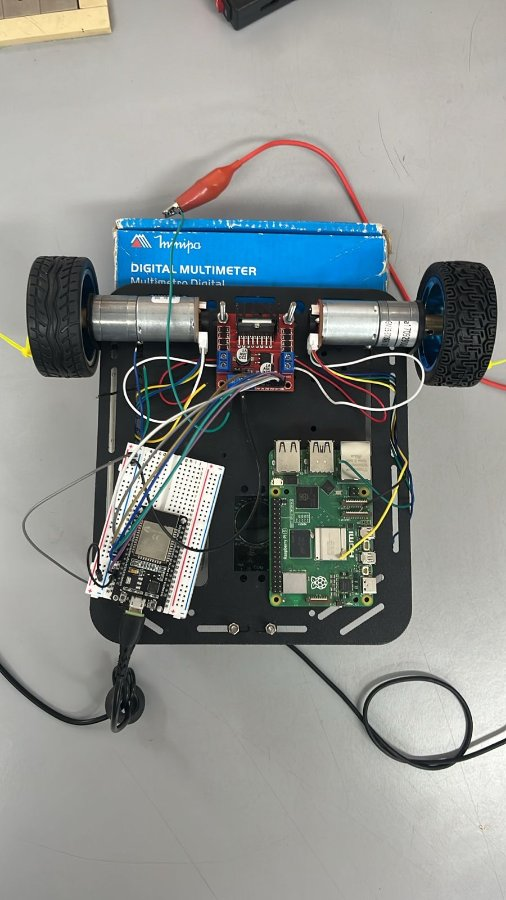
\includegraphics[height=0.74\textheight]{robot_3.jpg}
    \end{column}
    \begin{column}{0.27\textwidth}
      \centering
      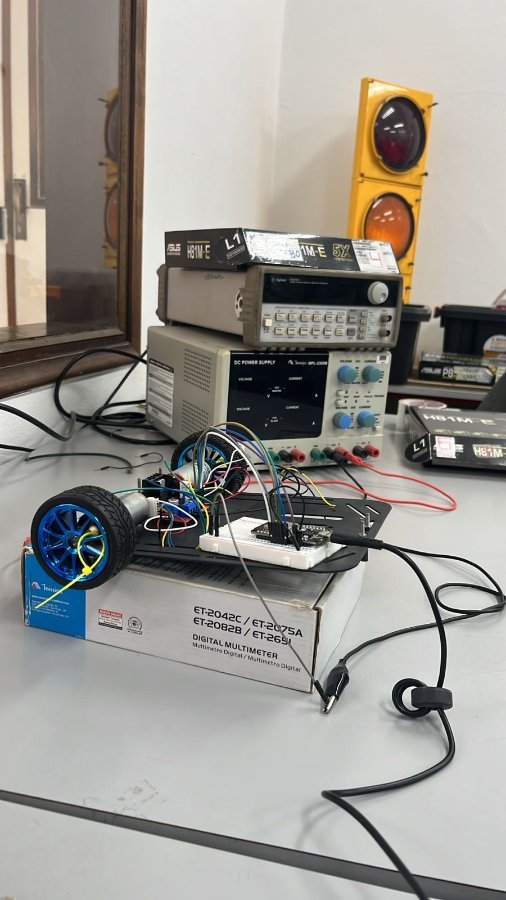
\includegraphics[height=0.74\textheight]{robot_2.jpg}
    \end{column}
    \begin{column}{0.42\textwidth}
      {\footnotesize
      \begin{block}{Qué se ve}
        \begin{itemize}
          \item Arriba, los dos motores con sus ruedas y, entre ellos, el
                módulo \textbf{L298N} (rojo).
          \item A la izquierda, el \textbf{ESP32} sobre una protoboard.
          \item A la derecha, la \textbf{Raspberry Pi 5}.
          \item El robot elevado sobre una caja: así se hicieron todas las
                pruebas hasta el 30 de septiembre.
        \end{itemize}
      \end{block}
      \begin{alertblock}{Lo que no se ve}
        Son fotos del banco. Falta la webcam, que va al frente, y las dos
        baterías. Las fotos del \textbf{robot terminado} están en la sección
        ``El 2 de octubre''.
      \end{alertblock}}
    \end{column}
  \end{columns}
\end{frame}

\begin{frame}{Alimentación: dos fuentes separadas}
  \centering
  \begin{tikzpicture}[font=\footnotesize, >={Stealth[length=2mm]},
      caja/.style={draw, rounded corners=2pt, minimum height=0.9cm, align=center,
                   line width=0.8pt, text width=2.6cm}]
    \node[caja, draw=azul, fill=azul!8] (carg) {Cargador portátil\\20 000 mAh, 5 V / 3 A};
    \node[caja, draw=azul, fill=azul!8, right=1.5cm of carg] (pi) {Raspberry Pi 5};
    \node[caja, draw=azul, fill=azul!8, right=1.3cm of pi, yshift=0.6cm] (cam) {Webcam USB};
    \node[caja, draw=azul, fill=azul!8, right=1.3cm of pi, yshift=-0.6cm] (esp) {ESP32};
    \node[caja, draw=naranja, fill=naranja!8, below=1.5cm of carg] (ups) {UPS 10 000 mAh\\salida de 12 V};
    \node[caja, draw=naranja, fill=naranja!8, right=1.5cm of ups] (l298) {L298N};
    \node[caja, draw=naranja, fill=naranja!8, right=1.3cm of l298] (mot) {Motores};
    \draw[->, azul, line width=0.9pt] (carg) -- node[above]{USB-A} (pi);
    \draw[->, azul, line width=0.9pt] (pi.east) -- (cam.west);
    \draw[->, azul, line width=0.9pt] (pi.east) -- (esp.west);
    \draw[->, naranja, line width=0.9pt] (ups) -- node[above]{12 V} (l298);
    \draw[->, naranja, line width=0.9pt] (l298) -- (mot);
    \draw[<->, gris, dashed, line width=0.8pt] (esp.south) -- ++(0,-0.55) -| node[pos=0.25, below]{6 señales + GND común} (l298.north);
  \end{tikzpicture}

  \vspace{0.3em}
  {\footnotesize
  \begin{columns}[T,onlytextwidth]
    \begin{column}{0.485\textwidth}
      \begin{block}{Por qué separadas}
        Con la UPS alimentando todo, la salida de 5 V se caía con la carga de
        YOLO \textbf{aun con los motores quietos}: mínimo 4,695 V, el Pi
        recortando el 43 \% del tiempo y el FPS de 11,2 a 8,83. Con el
        cargador aparte: 11,08 FPS y \cod{get_throttled = 0x0}.
      \end{block}
    \end{column}
    \begin{column}{0.485\textwidth}
      \begin{alertblock}{Tres cosas que no se tocan}
        \begin{itemize}
          \item El cargador va por \textbf{USB-A}. Por USB-C el Pi entra en
                bucle de reinicios.
          \item El \textbf{GND común} lo da el cableado ESP32--L298.
          \item Para cortar los motores se saca el \textbf{conector de 12 V},
                no la alimentación del Pi.
        \end{itemize}
      \end{alertblock}
    \end{column}
  \end{columns}}
\end{frame}

\begin{frame}{Cableado ESP32 $\leftrightarrow$ L298N}
  \relax{\footnotesize
  \begin{columns}[T,onlytextwidth]
    \begin{column}{0.52\textwidth}
      \begin{tabular}{L{1.6cm}L{1.3cm}L{3.6cm}}
        \toprule
        \textbf{L298N} & \textbf{GPIO} & \textbf{Función} \\
        \midrule
        ENA & 25 & PWM del canal A (\textbf{rueda derecha}) \\
        IN1 / IN2 & 26 / 27 & Sentido del canal A \\
        ENB & 13 & PWM del canal B (\textbf{rueda izquierda}) \\
        IN3 / IN4 & 33 / 32 & Sentido del canal B \\
        GND & GND & Referencia común \\
        \midrule
        Ultrasónico SIG & 12 & Con divisor 1 k / 2 k \\
        Buzzer & 14 & Activo, directo al pin \\
        \textcolor{grisclaro}{Encoders} & \textcolor{grisclaro}{34, 35, 36, 39} & \textcolor{grisclaro}{Reservados; sólo entrada} \\
        \bottomrule
      \end{tabular}
    \end{column}
    \begin{column}{0.44\textwidth}
      \begin{block}{PWM}
        1 kHz y \textbf{10 bits} (0 a 1023). Se pasó de 8 a 10 bits para darle
        resolución a la rueda izquierda, que usa una franja angosta del duty.
      \end{block}
      \begin{block}{Los canales quedaron cruzados}
        El canal A del módulo quedó cableado a la rueda \textbf{derecha}. No se
        tocó la bornera: se corrige en el firmware, en el bloque
        \cod{PIN_LEFT_*} / \cod{PIN_RIGHT_*}.
      \end{block}
      \begin{block}{Jumpers}
        Los de ENA y ENB van \textbf{retirados}: si no, el módulo deja los
        motores siempre habilitados y el PWM no hace nada.
      \end{block}
    \end{column}
  \end{columns}}

  \vspace{0.2em}
  {\footnotesize \ojo{El divisor del ultrasónico no es opcional:} el sensor
  contesta a 5 V y el ESP32 no los tolera. El detalle del cableado está en la
  sección ``El 2 de octubre''.}
\end{frame}

\begin{frame}{Los puertos USB del Pi importan}
  \begin{columns}[T,onlytextwidth]
    \begin{column}{0.485\textwidth}
      \begin{block}{Dónde va cada cosa}
        \begin{itemize}
          \item \textbf{Webcam}: USB \textbf{azul de abajo} (controlador 1).
          \item \textbf{ESP32}: USB \textbf{negro de abajo} (controlador 3),
                aparece como \cod{/dev/ttyUSB0}.
        \end{itemize}
        Quedan en controladores distintos. Compartiendo uno, el ruido de los
        motores rompía más la imagen.
      \end{block}
      \begin{block}{Formato de la cámara}
        \textbf{MJPG}, no YUYV. YUYV ocupa casi todo el ancho de banda del USB
        2.0 y no tolera pérdidas: con los motores andando daba 2,3 FPS e
        imagen en franjas. MJPG transmite $\sim$10 veces menos.
      \end{block}
    \end{column}
    \begin{column}{0.485\textwidth}
      \begin{alertblock}{El límite de corriente}
        Con el cargador portátil el Pi no negocia potencia y limita \textbf{todos
        sus USB a 600 mA}. La webcam declara 500 mA y el ESP32 100 mA: justo
        el total. Se puede levantar con \cod{usb_max_current_enable=1}
        (el cargador da 3 A). Está pendiente de probar.
      \end{alertblock}
      \begin{block}{Efecto colateral del puente USB}
        Abrir el puerto serie \textbf{reinicia el ESP32} (la línea DTR del
        CP2102). Por eso el enlace espera 2 s al abrir, y por eso leer
        telemetría ``para mirar'' frena los motores.
      \end{block}
    \end{column}
  \end{columns}
\end{frame}

\begin{frame}{El L298N: lo que dice la hoja de datos y lo que se midió}
  \begin{columns}[T,onlytextwidth]
    \begin{column}{0.485\textwidth}
      \begin{block}{La caída de tensión}
        El L298 es un puente de transistores bipolares: se queda con parte de
        la tensión. La hoja de datos sugería $\sim$1,4 V; \textbf{medido el
        2026-07-24: 2,5 V}. Con 12 V de entrada, a los motores les llegan
        $\sim$9,5 V.
      \end{block}
      \begin{block}{Consecuencia}
        Fue la primera de las estimaciones que la medición desmintió. A partir
        de ahí la regla del proyecto: \textbf{medir antes de creerle a la
        hoja de datos}.
      \end{block}
    \end{column}
    \begin{column}{0.485\textwidth}
      \begin{block}{Velocidad máxima real}
        Con rueda de 60 mm y 9,5 V en bornes: \textbf{0,87 m/s} a duty
        completo. A 5 FPS eso son 17 cm entre un frame y el siguiente:
        demasiado para controlar con visión. Por eso el robot usa sólo la
        parte baja del rango.
      \end{block}
      \begin{block}{Freno y rueda libre}
        Con las dos entradas de un canal al mismo nivel, el puente \textbf{frena}
        (cortocircuita el motor). El firmware frena 200 ms cuando salta el
        watchdog y después suelta a rueda libre, para no calentar el L298.
      \end{block}
    \end{column}
  \end{columns}
\end{frame}

\begin{frame}{Los motores: dos unidades que no son iguales}
  \begin{columns}[T,onlytextwidth]
    \begin{column}{0.44\textwidth}
      {\footnotesize
      \begin{block}{Lo que se midió (2026-08-27)}
        Ventanas de 10 s a duty fijo, contando vueltas:
        \begin{itemize}
          \item La rueda \textbf{izquierda} da \textbf{2,11 veces} más
                velocidad por cuenta de duty que la derecha.
          \item Y a la vez \textbf{cuesta más arrancarla}.
        \end{itemize}
      \end{block}
      \begin{block}{La explicación}
        Las dos cosas juntas no son fricción: son una \textbf{reducción menor}
        (relación $\sim$2,1:1 entre las dos cajas). Sólo la derecha coincide
        con la chapa de ``350 rpm''.
      \end{block}
      \begin{alertblock}{Lo que eso obliga}
        Cada rueda tiene \textbf{su propia recta} de duty a velocidad, con
        piso y techo propios. Un solo \cod{v_min} y un solo \cod{v_max} no
        alcanzan.
      \end{alertblock}}
    \end{column}
    \begin{column}{0.54\textwidth}
      \centering
      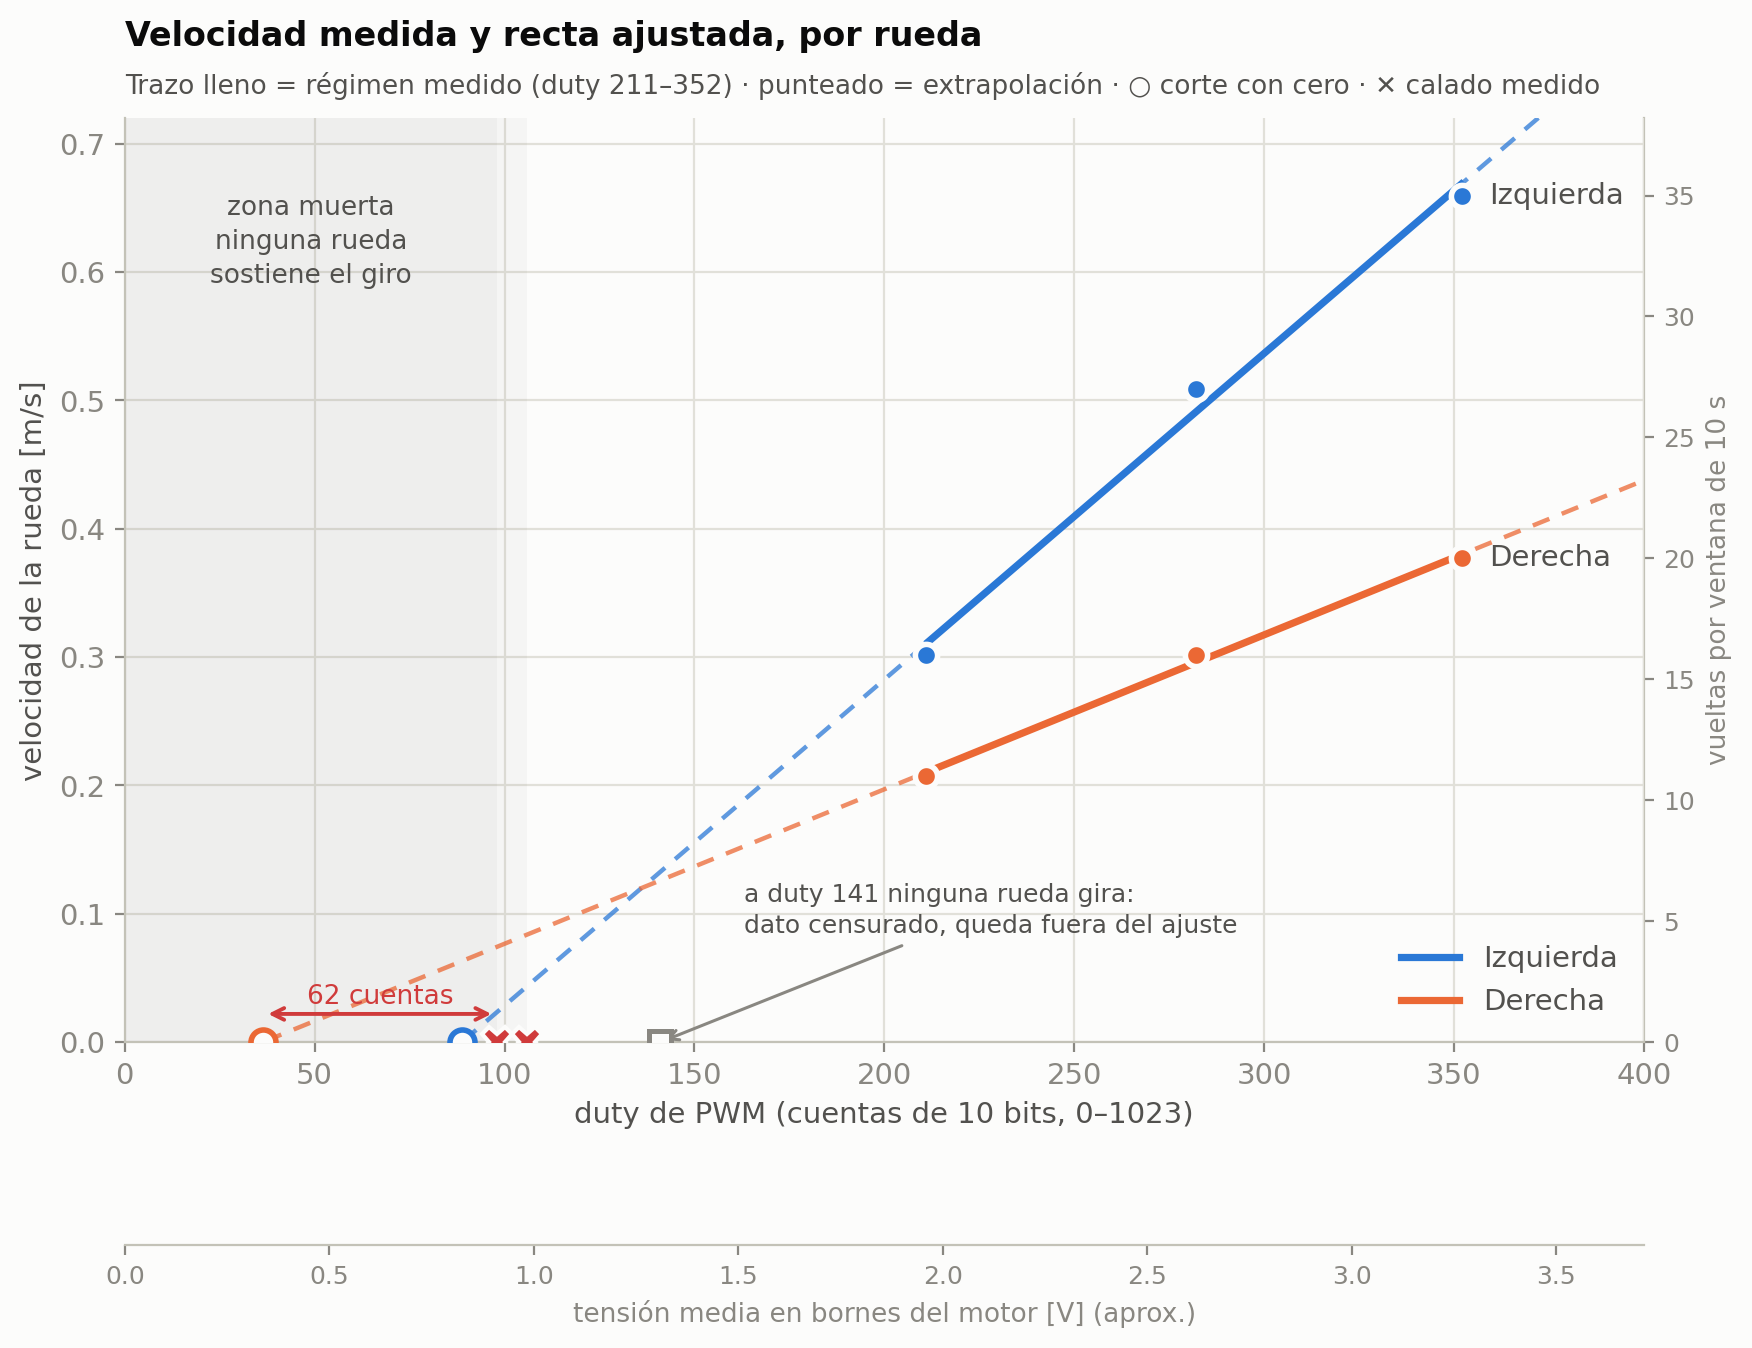
\includegraphics[width=0.93\textwidth]{fig1_rectas_calibracion.png}

      {\scriptsize Velocidad medida contra duty, por rueda. Azul: izquierda;
      naranja: derecha (cuaderno \cod{01_calibracion_motores.ipynb}).}
    \end{column}
  \end{columns}
\end{frame}

\begin{frame}{La calibración: una recta por rueda, con piso y techo}
  \centering
  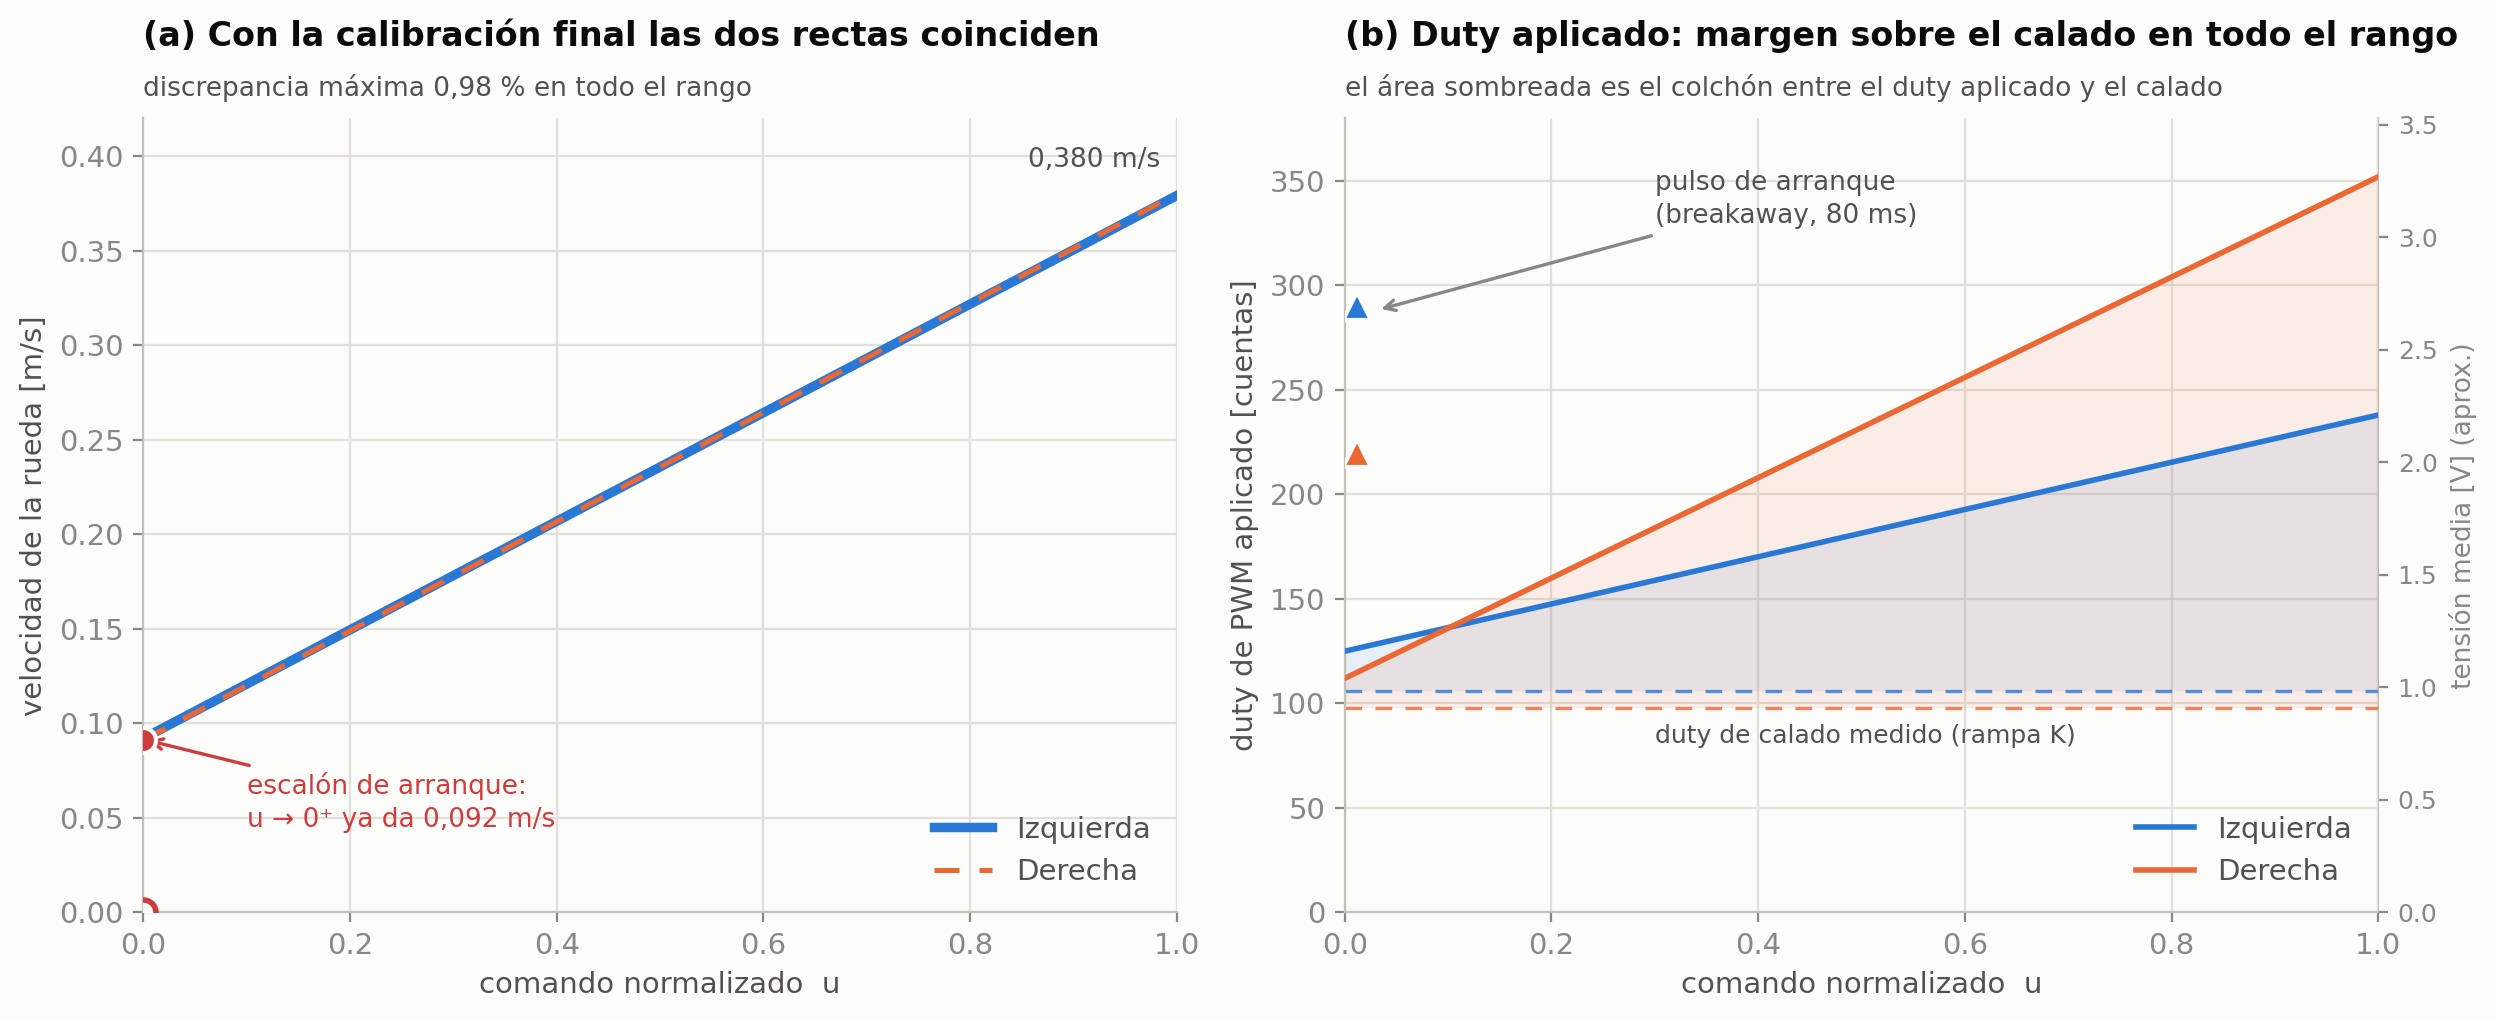
\includegraphics[width=0.64\textwidth]{fig3_calibracion_final.png}

  \vspace{0.2em}
  {\footnotesize
  \begin{columns}[T,onlytextwidth]
    \begin{column}{0.485\textwidth}
      \begin{block}{El mapa (en el ESP32)}
        Para un comando $u$ entre 0 y 1 de cada rueda:
        \[ \text{duty} = \text{PWM\_MIN} + (\text{PWM\_TOP} - \text{PWM\_MIN}) \cdot u \]
        y duty $= 0$ si $u = 0$. Con eso las dos ruedas siguen \textbf{la misma
        recta de velocidad}, con menos de 1 \% de diferencia.
      \end{block}
    \end{column}
    \begin{column}{0.485\textwidth}
      \begin{alertblock}{La consecuencia que más pesa}
        \textbf{No hay arranque suave.} Cualquier $u > 0$ da como mínimo
        \textbf{0,091 m/s}; un comando de 1 no hace ir ``despacito''. Para
        parar hay que mandar exactamente 0. De acá salen la zona muerta del
        control y varios de los problemas del piso.
      \end{alertblock}
    \end{column}
  \end{columns}}
\end{frame}

\begin{frame}{Calibración de banco contra calibración de piso}
  \relax{\footnotesize
  \begin{tabular}{L{3.6cm}L{2.6cm}L{2.6cm}L{4.7cm}}
    \toprule
    \textbf{Constante del firmware} & \textbf{Banco (27/08)} & \textbf{Piso (30/09)} & \textbf{Qué es} \\
    \midrule
    \cod{PWM_MIN} izq / der & 125 / 112 & \textbf{300 / 230} &
      Piso de la recta: el duty de la mínima velocidad sostenible \\[1pt]
    \cod{PWM_TOP} izq / der & 238 / 352 & \textbf{413 / 470} &
      Techo de la recta: el duty de $u = 1$ \\[1pt]
    \cod{PWM_BREAKAWAY} izq / der & 290 / 220 & \textbf{380 / 280} &
      Pulso de arranque, para vencer la fricción estática \\[1pt]
    \cod{BREAKAWAY_MS} & 80 ms & \textbf{150 ms} &
      Cuánto dura ese pulso \\
    \bottomrule
  \end{tabular}}

  \vspace{0.5em}
  \begin{columns}[T,onlytextwidth]
    \begin{column}{0.485\textwidth}
      \begin{alertblock}{Por qué hubo que rehacerla}
        {\footnotesize La de banco se hizo \textbf{con las ruedas al aire}. En el piso
        la rueda izquierda ---la de menos par, y encima la de menor duty--- se
        \textbf{calaba con cualquier comando}: los motores pitaban y el robot
        no giraba.}
      \end{alertblock}
    \end{column}
    \begin{column}{0.485\textwidth}
      \begin{block}{El modelo que funcionó}
        {\footnotesize La carga \textbf{suma un escalón de duty} (el par es
        corriente) y \textbf{no cambia la pendiente} (la velocidad es fuerza
        contraelectromotriz). Piso y techo suben lo mismo por rueda. Verificado:
        avance derecho, y 57 cm donde el modelo predecía 57.}
      \end{block}
    \end{column}
  \end{columns}

  \vspace{0.2em}
  {\footnotesize Las constantes \cod{PWM_*} de \cod{src/config.py} son una
  copia informativa: las que valen están en el firmware. Se pusieron al día
  con los valores de piso el 1 de octubre (en la PC; falta copiarlas al Pi).}
\end{frame}

\begin{frame}{La cámara}
  \begin{columns}[T,onlytextwidth]
    \begin{column}{0.485\textwidth}
      \begin{block}{Lo que quedó}
        \textbf{Webcam USB Microsoft LifeCam Studio} en \cod{/dev/video0}.
        Captura a 640$\times$480 en MJPG; la red trabaja a 320 px.
        \begin{itemize}
          \item Campo visual horizontal: \textbf{$\sim$52\grad} (estimado en el
                piso; se había supuesto 60).
          \item Alcance con el oso A4: \textbf{$\sim$1,3 m}.
          \item Montada al frente y muy baja (del orden de 10 cm del piso;
                no se midió). Ve los objetos desde abajo.
        \end{itemize}
      \end{block}
      \begin{block}{Lo que la cámara mide}
        No mide distancia: mide \textbf{tamaño aparente}. Por eso el objeto
        con el que se calibra es parte del número.
      \end{block}
    \end{column}
    \begin{column}{0.485\textwidth}
      \begin{alertblock}{Lo que no funcionó: la Arducam}
        La cámara prevista era una Arducam UC-609 (sensor IMX219, cable de 15
        pines) por el conector CSI. El Pi 5 \textbf{nunca la vio}: nada en
        \cod{dmesg}, nada en el bus I2C de los conectores, con las cuatro
        orientaciones del cable. Como ese sensor sí está en la autodetección,
        la falla era eléctrica. Se descartó \textbf{por tiempo, no por diseño}.
      \end{alertblock}
      \begin{block}{Dos cosas raras de la imagen}
        \begin{itemize}
          \item Girando de corrido sale \textbf{movida}: YOLO no ve nada.
          \item A ratos llega \textbf{en franjas}, aun con los motores
                parados. Causa sin aislar.
        \end{itemize}
      \end{block}
    \end{column}
  \end{columns}
\end{frame}

\begin{frame}{La Raspberry Pi 5}
  \relax{\footnotesize
  \begin{columns}[T,onlytextwidth]
    \begin{column}{0.485\textwidth}
      \begin{block}{Sistema}
        \begin{itemize}
          \item Raspberry Pi OS (Trixie), 64 bits, Python 3.13.
          \item Sin monitor ni teclado: se entra por SSH con la clave
                \cod{id_ed25519_pi}. Nombre \cod{pi-MB}, usuario \cod{admin}.
          \item Todo el proyecto vive en \cod{~/TPF/}: \cod{src/},
                \cod{scripts_pi/}, \cod{logs/} y el entorno \cod{.venv/}.
        \end{itemize}
      \end{block}
      \begin{block}{Entorno de Python}
        \cod{torch} 2.14, \cod{torchvision} 0.29, \cod{ultralytics} 8.4,
        \cod{opencv} 5.0 y \cod{pyserial}; todo instalado por rueda, nada
        compilado. El entorno pesa 5,6 GB, de los cuales 3,3 GB son librerías
        de CUDA que no se usan (pendiente de higiene).
      \end{block}
    \end{column}
    \begin{column}{0.485\textwidth}
      \begin{block}{Térmico}
        Con YOLO real corriendo 150 s: 2400 MHz y sin recortes, con meseta en
        \textbf{73--75 \grad C}. A 80 \grad C empieza a recortar. (Un test
        sintético de cuatro bucles vacíos sí lo hacía recortar: es más severo
        que la inferencia.)
      \end{block}
      \begin{block}{Cómo se le pregunta al Pi cómo está}
        \begin{itemize}
          \item \cod{vcgencmd get_throttled}: \cod{0x0} es todo bien. El bit 0
                es bajo voltaje ahora; el 16, que lo hubo desde el arranque.
          \item \cod{vcgencmd pmic_read_adc EXT5V_V}: la tensión de entrada
                (4,9 a 5,1 V).
          \item \cod{vcgencmd measure_temp}.
        \end{itemize}
      \end{block}
    \end{column}
  \end{columns}}
\end{frame}

% =============================================================================
\section{Arquitectura}
% =============================================================================

\begin{frame}{Dos niveles, con una frontera clara}
  \centering
  \begin{tikzpicture}[font=\footnotesize, >={Stealth[length=2mm]},
      b/.style={draw, rounded corners=2pt, minimum height=0.75cm, align=center,
                line width=0.8pt, text width=2.25cm, inner sep=2pt}]
    % Pi
    \node[b, draw=azul, fill=azul!8] (cam) {Cámara\\\cod{vision.Camara}};
    \node[b, draw=azul, fill=azul!8, right=0.35cm of cam] (yolo) {YOLOv8n\\\cod{vision.Detector}};
    \node[b, draw=azul, fill=azul!8, right=0.35cm of yolo] (conf) {Confirmación\\temporal};
    \node[b, draw=azul, fill=azul!8, right=0.35cm of conf] (est) {Máquina de\\estados};
    \node[b, draw=azul, fill=azul!8, right=0.35cm of est] (ctl) {Ley de\\control};
    \node[b, draw=azul, fill=azul!8, below=0.55cm of ctl] (enl) {Enlace serie\\\cod{enlace_esp32}};
    \node[b, draw=gris, fill=gris!8, below=0.55cm of conf] (reg) {Registro\\CSV + JSON};
    \begin{scope}[on background layer]
      \node[draw=azul, dashed, rounded corners=4pt, fit=(cam)(ctl)(enl)(reg), inner sep=7pt,
            label={[azul]above:\textbf{Raspberry Pi 5 --- alto nivel, $\sim$11 ciclos por segundo}}] (pibox) {};
    \end{scope}
    % ESP32
    \node[b, draw=naranja, fill=naranja!8, below=2.3cm of enl] (par) {Parser\\de líneas};
    \node[b, draw=naranja, fill=naranja!8, left=0.35cm of par] (mix) {Mezcla y\\zona muerta};
    \node[b, draw=naranja, fill=naranja!8, left=0.35cm of mix] (pwm) {PWM\\10 bits};
    \node[b, draw=gris, fill=gris!8, left=0.35cm of pwm] (l298) {L298N};
    \node[b, draw=gris, fill=gris!8, left=0.35cm of l298] (mot) {Motores};
    \node[b, draw=naranja, fill=naranja!8, above=0.3cm of mix] (wd) {Watchdog\\500 ms};
    \begin{scope}[on background layer]
      \node[draw=naranja, dashed, rounded corners=4pt, fit=(par)(pwm)(wd), inner sep=7pt,
            label={[naranja]below:\textbf{ESP32 --- bajo nivel, lazo de 100 Hz}}] (espbox) {};
    \end{scope}
    \draw[->] (cam) -- (yolo); \draw[->] (yolo) -- (conf); \draw[->] (conf) -- (est);
    \draw[->] (est) -- (ctl); \draw[->] (ctl) -- (enl); \draw[->] (est.south) |- (reg.east);
    \draw[->, line width=1pt] (enl) -- node[left, pos=0.2]{\cod{M,v_lin,v_ang} por USB-serie} (par);
    \draw[->] (par) -- (mix); \draw[->] (mix) -- (pwm); \draw[->] (pwm) -- (l298); \draw[->] (l298) -- (mot);
    \draw[->] (wd) -- (mix);
  \end{tikzpicture}

  \vspace{0.1em}
  {\footnotesize \textbf{El principio:} el Pi nunca toca un PWM y el ESP32 nunca
  decide un comportamiento. Cada nivel se depura por separado.}
\end{frame}

\begin{frame}{Qué sabe cada nivel, y qué ignora a propósito}
  \begin{columns}[T,onlytextwidth]
    \begin{column}{0.485\textwidth}
      \begin{block}{Raspberry Pi: la intención}
        \begin{itemize}
          \item Sabe qué hay en la imagen y qué conviene hacer.
          \item Habla en \textbf{intención normalizada}: avanzar y girar entre
                $-100$ y $100$.
          \item \textbf{Ignora} cuántas cuentas de PWM hacen falta, que las
                ruedas son distintas y que existe un puente H.
          \item No es de tiempo real: un ciclo tarda $\sim$90 ms y a veces más.
        \end{itemize}
      \end{block}
    \end{column}
    \begin{column}{0.485\textwidth}
      \begin{block}{ESP32: el hardware}
        \begin{itemize}
          \item Sabe traducir intención a duty, rueda por rueda, con la
                calibración medida.
          \item Garantiza que el robot \textbf{frena solo} si se queda sin
                órdenes.
          \item \textbf{Ignora} qué es un oso o una mochila, y en qué estado
                está el comportamiento.
          \item Sí es de tiempo real: su lazo corre cada 10 ms.
        \end{itemize}
      \end{block}
    \end{column}
  \end{columns}

  \vspace{0.5em}
  \begin{exampleblock}{Por qué la zona muerta se compensa en el ESP32}
    {\small Los pisos y techos de cada rueda están en \textbf{cuentas de PWM}, que es
    justo lo que el protocolo abstrae. Si se recalibra o se cambia un motor, se
    toca el firmware y \textbf{el Pi no se entera}. Fue lo que pasó el 30 de
    septiembre: se recalibró en el piso sin cambiar una línea de Python.}
  \end{exampleblock}
\end{frame}

\begin{frame}{La vida de un frame: de la foto a las ruedas}
  \centering
  \begin{tikzpicture}[font=\scriptsize, >={Stealth[length=1.8mm]},
      p/.style={draw, rounded corners=2pt, minimum height=1.0cm, align=center,
                line width=0.8pt, text width=1.7cm, inner sep=2pt}]
    \node[p, draw=azul, fill=azul!8] (a) {La cámara\\expone};
    \node[p, draw=azul, fill=azul!8, right=0.28cm of a] (b) {\cod{cam.leer()}\\saca el frame};
    \node[p, draw=azul, fill=azul!8, right=0.28cm of b] (c) {\cod{franjas()}\\salud de la imagen};
    \node[p, draw=azul, fill=azul!8, right=0.28cm of c] (d) {\cod{detectar()}\\YOLOv8n};
    \node[p, draw=azul, fill=azul!8, right=0.28cm of d] (e) {\cod{Confirmador}\\3 seguidos};
    \node[p, draw=azul, fill=azul!8, right=0.28cm of e] (f) {\cod{Maquina.paso()}\\decide};
    \node[p, draw=azul, fill=azul!8, right=0.28cm of f] (g) {\cod{esp.mover()}\\manda \cod{M}};
    \foreach \x/\y in {a/b,b/c,c/d,d/e,e/f,f/g} \draw[->] (\x) -- (\y);
    \node[below=0.15cm of a]  {36--64 ms};
    \node[below=0.15cm of b]  {0,6 ms};
    \node[below=0.15cm of c]  {1,7 ms};
    \node[below=0.15cm of d]  {\textbf{88 ms}};
    \node[below=0.15cm of e]  {$<$ 1 ms};
    \node[below=0.15cm of f]  {$<$ 1 ms};
    \node[below=0.15cm of g]  {en el acto};
  \end{tikzpicture}

  \vspace{0.5em}
  {\footnotesize
  \begin{columns}[T,onlytextwidth]
    \begin{column}{0.485\textwidth}
      \begin{block}{Lo que cuesta}
        Casi todo el ciclo es \textbf{la red}: 88 de $\sim$90 ms. La máquina de
        estados y el enlace cuestan alrededor del 1 \%. Por eso el tamaño de
        inferencia es la única palanca real del FPS.
      \end{block}
      \begin{block}{Después del comando}
        \cod{registro.fila()} escribe una línea del CSV y, si se pidió
        \cod{--grabar}, el frame anotado va al video.
      \end{block}
    \end{column}
    \begin{column}{0.485\textwidth}
      \begin{alertblock}{La latencia que no se ve}
        Sacar el frame de la cola tarda 0,6 ms, pero ese frame \textbf{ya
        tiene 36 a 64 ms de edad}. De foto a decisión pasan $\sim$150 ms; con
        el retardo de los motores, $\sim$0,25 s. A 0,25 m/s son unos 6 cm
        ``a ciegas''.
      \end{alertblock}
      \begin{block}{El orden importa}
        La salud de la imagen se mide \textbf{antes} de dibujar las cajas
        encima.
      \end{block}
    \end{column}
  \end{columns}}
\end{frame}

\begin{frame}{Tres relojes distintos, desacoplados}
  \relax{\footnotesize
  \begin{tabular}{L{3.1cm}L{2.3cm}L{8.4cm}}
    \toprule
    \textbf{Quién} & \textbf{Cadencia} & \textbf{Qué hace a ese ritmo} \\
    \midrule
    Lazo de visión (Pi) & $\sim$11 Hz, irregular &
      Un ciclo por frame: detectar, decidir, fijar el comando. Si un frame
      tarda, el ciclo tarda. \\[2pt]
    Latido del enlace (Pi, hilo aparte) & 10 Hz, regular &
      Repite el último comando al ESP32 \textbf{mientras siga fresco}. Si el
      comando \emph{cambia}, se manda en el acto sin esperar al latido. \\[2pt]
    Lector del enlace (Pi, hilo aparte) & lo que llegue &
      Lee la telemetría \cod{D,...} que el ESP32 manda a 20 Hz. \\[2pt]
    Lazo de control (ESP32) & 100 Hz &
      Revisa el watchdog y aplica el duty de cada rueda. \\[2pt]
    Telemetría (ESP32) & 20 Hz &
      Manda \cod{D,dist,enc_izq,enc_der}. Hoy siempre \cod{D,-1,0,0}. \\
    \bottomrule
  \end{tabular}}

  \vspace{0.6em}
  \begin{block}{Por qué hay un latido}
    {\small El ESP32 frena si pasa 500 ms sin un comando. El lazo de visión es
    irregular: un frame lento haría frenar el robot en medio de una maniobra.
    El latido desacopla las dos cadencias.}
  \end{block}
  \begin{alertblock}{Y por qué el latido no puede ser ingenuo}
    {\small Repetir el último comando \emph{para siempre} anularía el watchdog: si el
    lazo se cuelga, el hilo del latido seguiría diciendo ``andá''. Por eso sólo
    repite comandos con menos de 0,40 s de edad (\cod{VIGENCIA_COMANDO_S}).}
  \end{alertblock}
\end{frame}

\begin{frame}{Las dos reglas que ordenan el código}
  \begin{block}{Regla 1 --- Todos los parámetros viven en \cod{config.py}}
    Nada de constantes sueltas en el código. Cada valor lleva al lado
    \textbf{de dónde salió}: medido (con fecha), calculado o pendiente. Los
    días de piso se tocan muchas veces, y un número sin su contexto se usa mal.
  \end{block}

  \begin{block}{Regla 2 --- Las capas que deciden no tocan hardware}
    \begin{columns}[T,onlytextwidth]
      \begin{column}{0.48\textwidth}
        \textbf{Deciden} (funciones puras, reciben el tiempo por argumento):
        \begin{itemize}
          \item \cod{control.py}
          \item \cod{estados.py}
          \item \cod{vision.Confirmador}
        \end{itemize}
      \end{column}
      \begin{column}{0.48\textwidth}
        \textbf{Hablan con el mundo}:
        \begin{itemize}
          \item \cod{vision.Camara}, \cod{vision.Detector}
          \item \cod{enlace_esp32.py}
          \item \cod{main.py} (el cableado)
        \end{itemize}
      \end{column}
    \end{columns}
  \end{block}

  \begin{exampleblock}{Lo que eso compra}
    {\small El comportamiento entero se verifica \textbf{en la PC}, sin cámara, sin
    ESP32 y sin robot (\cod{prueba_estados.py}, 79 verificaciones), y se puede
    correr contra un robot simulado (\cod{simular_piso.py}). Así se encontró
    el bucle de huidas antes de que hubiera ruedas girando.}
  \end{exampleblock}
\end{frame}

\begin{frame}{Qué pasa cuando algo falla}
  \relax{\footnotesize
  \begin{tabular}{L{4.0cm}L{5.0cm}L{4.8cm}}
    \toprule
    \textbf{Falla} & \textbf{Quién reacciona} & \textbf{Resultado} \\
    \midrule
    El lazo de visión se cuelga (el programa sigue vivo) &
      El latido ve que el comando tiene más de 0,40 s y manda \cod{M,0,0} &
      Frena en menos de medio segundo \\[2pt]
    El programa muere, se corta el SSH o se desconecta el USB &
      El watchdog del ESP32: 500 ms sin \cod{M} &
      Freno activo 200 ms, después rueda libre \\[2pt]
    La cámara no entrega un frame &
      \cod{main.py} corta el lazo y sale por el camino normal &
      Frena al salir \\[2pt]
    Ctrl+C &
      Baja una bandera; el lazo termina su ciclo y sale del \cod{with Enlace} &
      Frena, cierra el CSV y el video \\[2pt]
    Una detección aislada falsa &
      El \cod{Confirmador} pide 3 frames seguidos &
      A lo sumo una pausa de un frame \\[2pt]
    La imagen llega rota &
      Nadie reacciona: \ojo{sólo se registra} (columna \cod{franjas}) &
      El robot queda ``ciego'' y sigue buscando \\[2pt]
    Un obstáculo en el camino &
      \ojo{Nadie}: no hay ultrasónico &
      Choca. Área despejada y alguien cerca \\
    \bottomrule
  \end{tabular}}

  \vspace{0.4em}
  {\footnotesize El corte que siempre funciona es físico: \textbf{sacar el
  conector de 12 V} de la UPS.}
\end{frame}

% =============================================================================
\section{El código del Pi, archivo por archivo}
% =============================================================================

\begin{frame}[fragile]{El mapa del proyecto}
\begin{columns}[T,onlytextwidth]
\begin{column}{0.47\textwidth}
\scriptsize
\begin{verbatim}
TPF/
  PLAN.md            plan y bitacora
  HARDWARE.md        analisis electrico
  RUNBOOK.md         paso a paso
  GUIA_PRESENTACION.md (+ .pdf)
  firmware/
    esp32_control/   firmware definitivo
    esp32_motor_test/  prueba de cableado
  src/               el codigo del Pi
  scripts_pi/        puesta en marcha
    piso/            pruebas en el piso
  scripts_auxiliares/  cuadernos
  presentacion/      arquitectura (agosto)
  presentacion_resumen/  este documento
  logs/              registros de corridas
  media/             video y evidencia
\end{verbatim}
\end{column}
\begin{column}{0.51\textwidth}
\footnotesize
\begin{block}{Los cuatro documentos}
  \begin{itemize}
    \item \cod{PLAN.md}: el estado actual (§1), la especificación (§6 a §8) y
          la \textbf{bitácora} de cada jornada (§13). Es el que manda.
    \item \cod{HARDWARE.md}: motores, L298, alimentación, cableado; cada
          medición con su fecha.
    \item \cod{RUNBOOK.md}: los pasos numerados para repetir cada cosa.
    \item \cod{GUIA_PRESENTACION.md}: cómo operar el robot sin ayuda el día de
          la presentación.
  \end{itemize}
\end{block}
\begin{block}{Dónde corre cada cosa}
  \cod{src/} y \cod{scripts_pi/} se copian al Pi, en \cod{~/TPF/}. El
  firmware se compila en la PC con PlatformIO. Los cuadernos y este documento
  viven sólo en la PC.
\end{block}
\end{column}
\end{columns}
\end{frame}

\begin{frame}{\cod{src/}: once archivos, tres familias}
  \relax{\footnotesize
  \begin{tabular}{L{3.0cm}L{1.0cm}L{9.7cm}}
    \toprule
    \textbf{Archivo} & \textbf{Líneas} & \textbf{Qué es} \\
    \midrule
    \multicolumn{3}{l}{\textbf{El robot} --- lo que corre en cada demo} \\
    \cod{config.py} & 484 & Todos los parámetros, cada uno con su origen \\
    \cod{vision.py} & 386 & Cámara, detector YOLO, confirmación temporal, salud de la imagen \\
    \cod{control.py} & 178 & La ley de control: de una caja a \cod{(v_lin, v_ang)} \\
    \cod{estados.py} & 349 & La máquina de estados: el comportamiento \\
    \cod{enlace_esp32.py} & 366 & El protocolo serie con el ESP32, el latido y la parada segura \\
    \cod{main.py} & 245 & El lazo principal: sólo cablea los anteriores \\
    \cod{registro.py} & 136 & El CSV y el JSON de cada corrida, y el video \\
    \midrule
    \multicolumn{3}{l}{\textbf{Las herramientas de medición}} \\
    \cod{bench_vision.py} & 423 & Mide el FPS real; modo ``en vivo'' para ver qué detecta \\
    \cod{analizar_corrida.py} & 305 & Saca las métricas de un CSV de corrida \\
    \midrule
    \multicolumn{3}{l}{\textbf{La verificación sin hardware}} \\
    \cod{prueba_estados.py} & 605 & 79 verificaciones del comportamiento, con el tiempo simulado \\
    \cod{simular_piso.py} & 318 & La máquina real contra un robot cinemático simulado \\
    \bottomrule
  \end{tabular}}

  \vspace{0.3em}
  {\footnotesize Más \cod{requirements.txt} y los pesos del modelo,
  \cod{yolov8n.pt}. Los nombres están en español, como el resto del proyecto.}
\end{frame}

\begin{frame}{Quién usa a quién}
  \centering
  \begin{tikzpicture}[font=\footnotesize, >={Stealth[length=2mm]},
      m/.style={draw, rounded corners=2pt, minimum height=0.7cm, align=center,
                line width=0.8pt, text width=2.3cm}]
    \node[m, draw=azul, fill=azul!12] (main) {\cod{main.py}};
    \node[m, draw=azul, fill=azul!8, below left=0.9cm and 3.6cm of main] (vis) {\cod{vision.py}};
    \node[m, draw=azul, fill=azul!8, below left=0.9cm and 0.1cm of main] (est) {\cod{estados.py}};
    \node[m, draw=azul, fill=azul!8, below right=0.9cm and 0.1cm of main] (enl) {\cod{enlace_esp32.py}};
    \node[m, draw=azul, fill=azul!8, below right=0.9cm and 3.6cm of main] (reg) {\cod{registro.py}};
    \node[m, draw=azul, fill=azul!8, below=0.8cm of est] (ctl) {\cod{control.py}};
    \node[m, draw=naranja, fill=naranja!10, below=2.9cm of main] (cfg) {\cod{config.py}};
    \draw[->] (main) -- (vis); \draw[->] (main) -- (est); \draw[->] (main) -- (enl); \draw[->] (main) -- (reg);
    \draw[->] (est) -- (ctl);
    \draw[->, dashed] (est) -- node[below=5pt, font=\scriptsize]{usa \cod{mejor()}} (vis);
    \draw[->, naranja] (ctl) -- (cfg); \draw[->, naranja] (vis.south) |- (cfg.west);
    \draw[->, naranja] (enl.south) |- ([yshift=2pt]cfg.east);
    \draw[->, naranja] (reg.south) |- ([yshift=-2pt]cfg.east);
  \end{tikzpicture}

  \vspace{0.4em}
  \relax{\footnotesize
  \begin{columns}[T,onlytextwidth]
    \begin{column}{0.485\textwidth}
      \begin{block}{Cómo leerlo}
        \cod{main.py} es el único que conoce a todos. Las flechas naranjas
        son ``lee sus parámetros de \cod{config.py}'': todos lo hacen.
      \end{block}
    \end{column}
    \begin{column}{0.485\textwidth}
      \begin{block}{Lo que \emph{no} hay}
        \cod{estados.py} y \cod{control.py} no importan ni la cámara ni el
        puerto serie. Por eso las herramientas de verificación los usan
        directamente, sin robot.
      \end{block}
    \end{column}
  \end{columns}}
\end{frame}

\begin{frame}{\cod{config.py} --- todos los números, con su historia}
  \relax{\footnotesize
  \begin{columns}[T,onlytextwidth]
    \begin{column}{0.485\textwidth}
      \begin{block}{Qué es}
        Un módulo de constantes, sin lógica (salvo dos funciones de
        conversión). Cada valor tiene al lado un comentario que dice
        \textbf{de dónde salió}: medido (con fecha), calculado, o pendiente.
        Más de la mitad del archivo son esos comentarios.
      \end{block}
      \begin{block}{Sus secciones}
        \begin{enumerate}\setcounter{enumi}{-1}
          \item Rutas (\cod{DIR_LOGS}, \cod{DIR_MEDIA}).
          \item Cámara.
          \item Detección (modelo, clases, umbrales, confirmación).
          \item Ley de control y \cod{BUSCAR}.
          \item Tracción (lo que hace el firmware, replicado).
          \item Estados: \cod{HUIR} y ultrasónico.
          \item Enlace serie.
          \item Métricas.
        \end{enumerate}
      \end{block}
    \end{column}
    \begin{column}{0.485\textwidth}
      \begin{block}{Las dos funciones}
        \begin{itemize}
          \item \cod{velocidad_real(u)}: de un comando $u$ entre 0 y 1 a m/s,
                con el escalón de arranque:
                $v = 0{,}0915 + 0{,}289\,u$ para $u > 0$.
          \item \cod{comando_para_velocidad(v)}: la inversa.
        \end{itemize}
      \end{block}
      \begin{block}{Las marcas de los comentarios}
        Tilde verde: medido. Cuadrado vacío: puesto a ojo, falta medir.
        Círculo rojo: una trampa que ya costó una jornada.
      \end{block}
      \begin{exampleblock}{Cómo se cambia un parámetro para una sola corrida}
        \cod{corrida_piso.sh etiqueta 25 "nota" KP_ANG=0.4}: lo cambia, corre,
        y lo restaura al terminar.
      \end{exampleblock}
    \end{column}
  \end{columns}}
\end{frame}

\begin{frame}{\cod{vision.py} (1 de 2) --- de un frame a una lista de detecciones}
  \relax{\footnotesize
  \begin{columns}[T,onlytextwidth]
    \begin{column}{0.485\textwidth}
      \begin{block}{\cod{Deteccion} (un dato inmutable)}
        Una caja ya convertida a lo que el control necesita:
        \cod{clase}, \cod{conf}, la caja en píxeles (\cod{x, y, w, h}) y los
        dos números de la ley de control:
        \begin{itemize}
          \item \cod{error_x}: de $-1$ (borde izquierdo) a $+1$ (derecho).
          \item \cod{area_ratio}: fracción de la imagen que ocupa la caja.
        \end{itemize}
      \end{block}
      \begin{block}{\cod{Detector}}
        Envuelve a YOLOv8n. Al construirse resuelve los \textbf{nombres} de
        las clases contra \cod{model.names}; si el modelo no las conoce, falla
        ahí. \cod{detectar(frame)} devuelve la lista de \cod{Deteccion} y los
        tiempos de inferencia y posproceso.
      \end{block}
    \end{column}
    \begin{column}{0.485\textwidth}
      \begin{block}{Dos cosas que agregó el piso}
        \begin{itemize}
          \item \textbf{Alias} (\cod{ALIAS_CLASES}): lo que el modelo llama
                \cod{suitcase} sale del detector ya renombrado a
                \cod{backpack}. El resto del sistema no se entera.
          \item \textbf{Umbral por clase} (\cod{UMBRAL_POR_CLASE}): a YOLO se
                le pide con el umbral más bajo y cada caja se filtra con el de
                su clase (0,20 la mochila, 0,35 el oso).
        \end{itemize}
      \end{block}
      \begin{block}{Otros detalles}
        \begin{itemize}
          \item \cod{calentar()}: tres inferencias de descarte. La primera
                tarda varias veces lo normal.
          \item El filtrado por clase lo hace la propia librería
                (\cod{classes=...}): no se procesan las otras 78 clases.
        \end{itemize}
      \end{block}
    \end{column}
  \end{columns}}
\end{frame}

\begin{frame}{\cod{vision.py} (2 de 2) --- confirmación, cámara y salud de la imagen}
  \relax{\footnotesize
  \begin{columns}[T,onlytextwidth]
    \begin{column}{0.485\textwidth}
      \begin{block}{\cod{Confirmador}}
        Lleva, por clase, cuántos frames seguidos se la vio y cuántos no.
        \cod{actualizar(clases)} devuelve el conjunto de clases
        \textbf{confirmadas}: entra con 3 frames seguidos
        (\cod{N_CONFIRMAR}), sale con 5 sin verla (\cod{M_PERDER}).
      \end{block}
      \begin{block}{\cod{mejor(detecciones, clase)}}
        La caja más confiable de una clase, o \cod{None}. Es lo único de este
        módulo que usa la máquina de estados.
      \end{block}
      \begin{block}{\cod{dibujar()}}
        Anota el frame con las cajas y el estado. Sólo para el video y para
        depurar.
      \end{block}
    \end{column}
    \begin{column}{0.485\textwidth}
      \begin{block}{\cod{Camara}}
        Abstrae las dos cámaras posibles: CSI (Picamera2) o USB (OpenCV sobre
        V4L2). Hoy siempre USB. Fija \textbf{primero el formato} (MJPG) y
        después el tamaño, y pide un búfer de un solo frame para no trabajar
        sobre imágenes viejas.
      \end{block}
      \begin{block}{\cod{franjas(frame)}}
        Fracción de las filas que son una \textbf{franja gris uniforme}: lo
        que deja un paquete USB perdido en un frame MJPG. 0,0 es un frame
        sano; arriba de 0,10 la detección ya no es confiable. Cuesta 1,7 ms y
        va a cada fila del registro.
      \end{block}
    \end{column}
  \end{columns}}
\end{frame}

\begin{frame}{\cod{control.py} --- la ley de control, en funciones puras}
  \relax{\footnotesize
  \begin{columns}[T,onlytextwidth]
    \begin{column}{0.485\textwidth}
      \begin{block}{Qué es}
        Convierte una detección en un comando. Nada más: no toca la cámara, no
        toca el puerto y no recuerda nada entre llamadas.
      \end{block}
      \begin{block}{Las funciones}
        \begin{itemize}
          \item \cod{girar_hacia(error_x)} \hacia{} \cod{v_ang}, con zona
                muerta.
          \item \cod{avanzar_hacia(area_ratio)} \hacia{} \cod{v_lin}, nunca
                negativo.
          \item \cod{perseguir(deteccion)} \hacia{} las dos, con el giro
                \textbf{acotado} a 0,7 veces el avance.
          \item \cod{a_protocolo()}: de normalizado a entero entre $-100$ y
                $100$, con tope.
        \end{itemize}
      \end{block}
    \end{column}
    \begin{column}{0.485\textwidth}
      \begin{block}{Las de diagnóstico}
        \begin{itemize}
          \item \cod{techo_efectivo_lineal()}: cuál es el \cod{v_lin} máximo
                que la ley puede pedir, y \textbf{cuál de los dos límites
                manda} (la ganancia o \cod{V_LIN_MAX}).
          \item \cod{kp_lin_para_saturar()}: la ganancia mínima para que
                mande \cod{V_LIN_MAX}.
          \item \cod{describir()}: el resumen que \cod{main.py} imprime al
                arrancar.
        \end{itemize}
      \end{block}
      \begin{exampleblock}{Se puede correr solo}
        \cod{python control.py} imprime una tabla de \cod{error_x} a
        \cod{v_ang} y de \cod{area_ratio} a \cod{v_lin} con los parámetros
        vigentes. Sirve para ver qué va a pedir la ley antes de soltar el robot.
      \end{exampleblock}
    \end{column}
  \end{columns}}
\end{frame}

\begin{frame}{\cod{estados.py} --- el comportamiento}
  \relax{\footnotesize
  \begin{columns}[T,onlytextwidth]
    \begin{column}{0.485\textwidth}
      \begin{block}{\cod{Comando}}
        Lo que la máquina pide en un ciclo: \cod{v_lin}, \cod{v_ang},
        \cod{buzzer} (casi siempre \cod{None}), \cod{estado} y un
        \cod{motivo} en texto. El motivo es lo que aparece en la consola y en
        el CSV: ``barriendo'', ``posible objetivo, freno a confirmar''...
      \end{block}
      \begin{block}{\cod{Maquina.paso(...)}}
        Un ciclo de decisión. Recibe las clases confirmadas, las detecciones
        crudas del frame, la telemetría del ESP32 y \textbf{la hora}; devuelve
        un \cod{Comando}. No lee ningún reloj por su cuenta.
      \end{block}
    \end{column}
    \begin{column}{0.485\textwidth}
      \begin{block}{Lo que la máquina recuerda}
        \begin{itemize}
          \item \cod{estado} y \cod{entrado_en}: en qué estado está y desde
                cuándo.
          \item \cod{fase_huir}: 1, 2 o 3.
          \item \cod{lado_amenaza}: de qué lado estaba la mochila.
          \item \cod{huida_termino_en}: para el período sordo.
          \item \cod{sentido_barrido}: hacia dónde gira al buscar.
        \end{itemize}
      \end{block}
      \begin{block}{Un método por estado}
        \cod{_buscar}, \cod{_aproximar}, \cod{_huir}, \cod{_encontrado}. El
        detalle de cada uno está en la sección ``La máquina de estados''.
      \end{block}
    \end{column}
  \end{columns}}
\end{frame}

\begin{frame}{\cod{enlace_esp32.py} --- la única pieza que sabe que hay un cable}
  \relax{\footnotesize
  \begin{columns}[T,onlytextwidth]
    \begin{column}{0.485\textwidth}
      \begin{block}{\cod{Enlace}}
        Abre el puerto, espera 2 s a que el ESP32 termine de reiniciarse y
        lanza \textbf{dos hilos}:
        \begin{itemize}
          \item \emph{lector}: lee líneas, descarta las que empiezan con
                \texttt{\#} y guarda la última telemetría.
          \item \emph{latido}: cada 0,1 s manda el comando vigente, o
                \cod{M,0,0} si ya venció.
        \end{itemize}
      \end{block}
      \begin{block}{Lo que se le pide}
        \begin{itemize}
          \item \cod{mover(v_lin, v_ang)}: fija el comando. Si cambió, lo manda
                \textbf{en el acto}.
          \item \cod{parar()}: \cod{M,0,0} ya.
          \item \cod{buzzer(patron)}: un evento, se manda una vez.
          \item \cod{estado}: la última telemetría.
        \end{itemize}
      \end{block}
    \end{column}
    \begin{column}{0.485\textwidth}
      \begin{block}{\cod{EstadoESP32}}
        La última línea \cod{D} interpretada. \cod{dist_cm} es \cod{None}
        cuando el ESP32 manda $-1$ (``sin lectura''); \cod{obstaculo()} trata
        el ``no sé'' como ``no''. Hoy siempre es ``no sé''.
      \end{block}
      \begin{block}{Para probar sin ESP32}
        \cod{Enlace(simular=True)} usa un puerto de mentira que contesta
        \cod{D,-1,0,0} y guarda lo que se le escribe. Es lo que usa
        \cod{main.py --simular}.
      \end{block}
      \begin{alertblock}{Sale siempre frenando}
        Se usa con \cod{with}: al salir manda \cod{M,0,0}, aunque haya habido
        una excepción.
      \end{alertblock}
    \end{column}
  \end{columns}}
\end{frame}

\begin{frame}[fragile]{\texttt{main.py} --- el lazo, que es sólo cableado}
\begin{columns}[T,onlytextwidth]
\begin{column}{0.53\textwidth}
\scriptsize
\begin{verbatim}
cam, det = Camara(), Detector()
conf, maq = Confirmador(), Maquina()
with Enlace() as esp:
    det.calentar(cam.leer())
    esperar(--espera)          # soltar el robot
    reg = Registro(...)
    while seguir:
        frame = cam.leer()
        rotas = franjas(frame)
        dets  = det.detectar(frame)
        confirmadas = conf.actualizar(dets)
        cmd = maq.paso(confirmadas, dets,
                       esp.estado, ahora)
        esp.mover(cmd.v_lin, cmd.v_ang)
        if cmd.buzzer: esp.buzzer(cmd.buzzer)
        reg.fila(..., rotas)
        if tiempo >= --duracion: break
# al salir del with: M,0,0
\end{verbatim}
\end{column}
\begin{column}{0.45\textwidth}
\footnotesize
\begin{tabular}{L{2.1cm}L{3.9cm}}
  \toprule
  \textbf{Opción} & \textbf{Qué hace} \\
  \midrule
  \verb|--duracion N| & Para solo a los N segundos. \textbf{Siempre ponerla.} \\
  \verb|--espera N| & Segundos antes de arrancar \\
  \verb|--simular| & No habla con el ESP32 \\
  \verb|--silencioso| & Una línea cada 10 ciclos \\
  \verb|--nota "..."| & Qué escenario es; va al JSON \\
  \verb|--grabar| & Video anotado (baja $\sim$1 FPS) \\
  \verb|--sin-registro| & No escribe el CSV \\
  \verb|--tam N| & Otro tamaño de inferencia \\
  \verb|--puerto P| & Otro puerto serie \\
  \verb|--preview| & Ventana (no sirve por SSH) \\
  \bottomrule
\end{tabular}

\vspace{0.3em}
Ctrl+C no mata el proceso: baja una bandera y el lazo sale por su camino
normal, que es el que frena.
\end{column}
\end{columns}
\end{frame}

\begin{frame}{\cod{registro.py} --- lo que queda de cada corrida}
  \relax{\footnotesize
  \begin{columns}[T,onlytextwidth]
    \begin{column}{0.56\textwidth}
      \begin{tabular}{L{2.9cm}L{4.7cm}}
        \toprule
        \textbf{Columna del CSV} & \textbf{Qué guarda} \\
        \midrule
        \cod{t_s}, \cod{dt_ms} & Tiempo desde el arranque y duración del ciclo \\
        \cod{estado}, \cod{fase_huir} & Estado de la máquina \\
        \cod{v_lin}, \cod{v_ang}, \cod{buzzer} & El comando enviado \\
        \cod{confirmadas} & Clases confirmadas, separadas por barra \\
        \cod{n_det} & Cuántas cajas hubo en el frame \\
        \cod{franjas} & Salud de la imagen (0 es sana) \\
        \cod{obj_conf/ex/ar/w/h} & La mejor caja \textbf{cruda} del oso \\
        \cod{amz_conf/ex/ar} & La mejor caja cruda de la mochila \\
        \cod{dist_cm} & Ultrasónico (vacío: sin lectura) \\
        \cod{motivo} & Por qué se mandó ese comando \\
        \bottomrule
      \end{tabular}
    \end{column}
    \begin{column}{0.42\textwidth}
      \begin{block}{Dos archivos por corrida}
        \cod{corrida_AAAAMMDD_HHMMSS.csv} con una fila por ciclo, y un
        \cod{.json} con \textbf{los parámetros de esa corrida} y la nota. Un
        CSV sin sus parámetros es un número sin contexto.
      \end{block}
      \begin{block}{Y el video}
        Con \cod{--grabar}, un \cod{.avi} con el frame anotado de cada ciclo:
        el frame $k$ del video es la fila $k$ del CSV.
      \end{block}
      \begin{block}{Por qué la caja cruda}
        Guardar la caja confirmada \emph{o no} permite medir cuánto tardó la
        confirmación desde el primer avistamiento.
      \end{block}
    \end{column}
  \end{columns}}
\end{frame}

\begin{frame}{\cod{analizar_corrida.py} --- del CSV a las métricas}
  \relax{\footnotesize
  \begin{columns}[T,onlytextwidth]
    \begin{column}{0.485\textwidth}
      \begin{block}{Qué informa de una corrida}
        \begin{itemize}
          \item \textbf{Lazo}: FPS, y duración del ciclo (mediana, percentil
                95 y máximo).
          \item \textbf{Imagen}: frames con franjas; avisa ``cámara a ciegas''
                si más del 20 \% están muy dañados.
          \item \textbf{Estados}: tiempo en cada uno y cada transición.
          \item \textbf{Buscar}: cuánto tardó en confirmar desde que lo vio, y
                si el oso seguía en la imagen medio segundo después.
          \item \textbf{Aproximar}: error lateral (RMS y máximo), cruces de
                lado y pérdidas del objetivo.
          \item \textbf{Encontrado}: con qué área frenó y con cuál quedó.
          \item \textbf{Huir}: latencia de reacción y frames con mochila.
        \end{itemize}
      \end{block}
    \end{column}
    \begin{column}{0.485\textwidth}
      \begin{block}{Con varias corridas}
        \cod{python analizar_corrida.py logs/corrida_*.csv} arma una tabla con
        una línea por corrida y el resumen: cuántas llegaron a
        \cod{ENCONTRADO} y el tiempo medio. Es la herramienta para las 10
        corridas por escenario.
      \end{block}
      \begin{alertblock}{Lo que el CSV no puede decir}
        La distancia \textbf{real} a la que frenó, si chocó, y cuánto giró de
        verdad. El registro sabe qué pidió el Pi y qué vio la cámara; no sabe
        dónde quedó el robot. Eso se anota a mano, con cinta métrica.
      \end{alertblock}
      \begin{block}{Dependencias}
        Sólo la biblioteca estándar: corre igual en el Pi y en la PC.
      \end{block}
    \end{column}
  \end{columns}}
\end{frame}

\begin{frame}{\cod{prueba_estados.py} --- 79 verificaciones sin robot}
  \relax{\footnotesize
  \begin{columns}[T,onlytextwidth]
    \begin{column}{0.52\textwidth}
      \begin{tabular}{L{0.4cm}L{6.5cm}}
        \toprule
        & \textbf{Qué verifica cada grupo} \\
        \midrule
        1 & \cod{BUSCAR}: barre, se reubica, alterna mirar y girar \\
        2 & \cod{APROXIMAR}: frena al acercarse, gira al lado correcto, llega \\
        3 & Pérdida del objetivo, y que lo busca por donde lo vio \\
        4 & \cod{HUIR} tiene prioridad sobre todo \\
        5 & Las tres fases de \cod{HUIR}, en orden y sin reevaluar \\
        6 & El período sordo después de huir \\
        7 & El ultrasónico: obstáculo propio contra ajeno \\
        8 & Frenar el barrido al primer avistamiento \\
        9 & Todo lo que sale entra en el protocolo \\
        \bottomrule
      \end{tabular}
    \end{column}
    \begin{column}{0.46\textwidth}
      \begin{block}{Cómo funciona}
        Una clase \cod{Escenario} corre la máquina con un \textbf{reloj
        simulado} y detecciones inventadas, y junta los comandos que fueron
        saliendo. Corre en un segundo, en cualquier máquina.
      \end{block}
      \begin{block}{Para qué sirvió}
        Encontró, antes de que hubiera ruedas girando, que las huidas se
        reencadenaban solas. Y \cod{demo.sh chequeo} la corre antes de cada
        demo.
      \end{block}
      \begin{alertblock}{Lo que no garantiza}
        Que la decisión verificada sea \emph{buena}. Una de estas
        verificaciones exigía, hasta el 1 de octubre, justo lo que hacía que
        el robot no huyera.
      \end{alertblock}
    \end{column}
  \end{columns}}
\end{frame}

\begin{frame}{\cod{simular_piso.py} y \cod{bench_vision.py}}
  \relax{\footnotesize
  \begin{columns}[T,onlytextwidth]
    \begin{column}{0.485\textwidth}
      \begin{block}{\cod{simular_piso.py}: predecir antes de soltar el robot}
        Corre la \textbf{máquina y el confirmador reales} contra un robot
        diferencial simulado. Lo que se simula es el mundo; lo que decide es
        el mismo código del Pi.
        \begin{itemize}
          \item \textbf{Medido}: calibración de motores, FPS, edad del frame,
                alcance.
          \item \textbf{Estimado}: trocha, campo visual.
          \item \textbf{Supuesto}: inercia, probabilidad de detección.
        \end{itemize}
        Predijo que el barrido de corrido iba a fallar si la imagen se movía.
        Sirve para comparar variantes, no para creerle los números absolutos.
      \end{block}
    \end{column}
    \begin{column}{0.485\textwidth}
      \begin{block}{\cod{bench_vision.py}: cuánto rinde la visión}
        Mide el FPS real de cámara más red, barriendo tamaños de inferencia y
        separando captura, inferencia y posproceso.
        \begin{itemize}
          \item Sin argumentos: el barrido, con resultados en \cod{logs/}.
          \item \cod{--en-vivo}: imprime lo que detecta frame a frame y
                guarda la foto anotada en \cod{logs/vivo.jpg}. Es lo que usa
                \cod{demo.sh ver}.
          \item Tiene una cámara sintética para medir sin cámara conectada.
        \end{itemize}
        De acá salió \cod{TAM_INFERENCIA = 320}.
      \end{block}
    \end{column}
  \end{columns}}
\end{frame}

% =============================================================================
\section{El firmware del ESP32}
% =============================================================================

\begin{frame}{Qué es y qué no es}
  \relax{\footnotesize
  \begin{columns}[T,onlytextwidth]
    \begin{column}{0.485\textwidth}
      \begin{block}{Dónde está}
        \cod{firmware/esp32_control/src/main.cpp}: un solo archivo de unas
        1360 líneas, en C con el marco de Arduino, compilado con PlatformIO.
        La carpeta \cod{firmware/} es un repositorio git aparte.
      \end{block}
      \begin{block}{Qué hace}
        \begin{itemize}
          \item Recibe intención de movimiento por el puerto serie.
          \item La traduce a duty de PWM, rueda por rueda.
          \item Frena solo si se queda sin órdenes.
          \item Devuelve telemetría 20 veces por segundo.
          \item Ofrece un modo manual y un modo de calibración para trabajar
                sin el Pi.
        \end{itemize}
      \end{block}
    \end{column}
    \begin{column}{0.485\textwidth}
      \begin{block}{Qué no hace}
        \textbf{No decide nada}. No sabe qué es un oso, ni en qué estado está
        el comportamiento. Si el Pi le pide algo absurdo, lo ejecuta (acotado
        a $\pm 100$).
      \end{block}
      \begin{block}{El otro firmware}
        \cod{esp32_motor_test/} fue el de la prueba de cableado de julio:
        mover los motores con teclas. Quedó como registro; no se usa.
      \end{block}
      \begin{block}{Cómo saber qué firmware tiene cargado}
        \cod{demo.sh firmware} le pide sus parámetros. Tiene que decir
        \cod{v_min izq/der: 300 / 230}. Si dice \cod{125 / 112} es el de
        banco, con el que la rueda izquierda no se mueve apoyada.
      \end{block}
    \end{column}
  \end{columns}}
\end{frame}

\begin{frame}[fragile]{El lazo principal del ESP32}
\begin{columns}[T,onlytextwidth]
\begin{column}{0.50\textwidth}
\footnotesize
\begin{verbatim}
loop():
  serial_poll()      # lee lineas, las procesa
  ping_poll()        # recoge el eco (ultrasonico)
  buzz_update()      # avanza el patron del buzzer
  ramp_update()      # calibracion: rampa K
  window_update()    # calibracion: ventana V

  cada 60 ms:  ping_send()
  cada 10 ms:                       # 100 Hz
      watchdog_update()
      si esta en calibracion:
          duty crudo, sin compensar
      si no esta frenando el watchdog:
          wheel_apply(izquierda)
          wheel_apply(derecha)
  cada 50 ms:  telemetry_send()     # 20 Hz
\end{verbatim}
\end{column}
\begin{column}{0.48\textwidth}
\footnotesize
\begin{block}{Nada bloquea}
  No hay ningún \verb|delay()| en el lazo. Cada tarea mira el reloj y hace su
  parte si le toca. El ultrasónico se mide \textbf{por interrupción}: un
  \verb|pulseIn()| con 30 ms de espera habría trabado un lazo de 10 ms.
\end{block}
\begin{block}{Qué pasa cuando llega una línea}
  \verb|serial_poll()| junta caracteres hasta el salto de línea y llama a
  \verb|process_line()|, que distingue:
  \begin{itemize}
    \item \verb|M,...| y \verb|B,...|: el protocolo.
    \item \verb|K|, \verb|V|, \verb|C|: calibración.
    \item una letra sola: modo manual.
  \end{itemize}
  Un \verb|M| guarda el comando de cada rueda y pone el watchdog en cero.
\end{block}
\end{column}
\end{columns}
\end{frame}

\begin{frame}{De \cod{M,v_lin,v_ang} al duty de cada rueda}
  \centering
  \begin{tikzpicture}[font=\footnotesize, >={Stealth[length=2mm]},
      p/.style={draw=naranja, fill=naranja!8, rounded corners=2pt, minimum height=1.05cm,
                align=center, line width=0.8pt, text width=2.75cm, inner sep=2pt}]
    \node[p] (a) {\cod{mix()}\\izq $= v_{lin} + v_{ang}$\\der $= v_{lin} - v_{ang}$};
    \node[p, right=0.5cm of a] (b) {\cod{deadzone_map()}\\duty $=$ min $+$ (top $-$ min)$\cdot u$};
    \node[p, right=0.5cm of b] (c) {\cod{wheel_apply()}\\pulso de arranque\\los primeros 150 ms};
    \node[p, right=0.5cm of c] (d) {\cod{wheel_raw()}\\sentido en IN1..IN4\\duty en el PWM};
    \draw[->] (a) -- (b); \draw[->] (b) -- (c); \draw[->] (c) -- (d);
  \end{tikzpicture}

  \vspace{0.4em}
  \relax{\footnotesize
  \begin{tabular}{L{2.0cm}L{2.5cm}L{2.5cm}L{6.4cm}}
    \toprule
    \textbf{Comando} & \textbf{Rueda izquierda} & \textbf{Rueda derecha} & \textbf{Qué hace el robot} \\
    \midrule
    \cod{M,55,0} & $+55$ \hacia{} duty 362 & $+55$ \hacia{} duty 362 &
      Avanza derecho a 0,25 m/s. El mismo duty es casualidad: las rectas se cruzan ahí \\[1pt]
    \cod{M,0,35} & $+35$ \hacia{} duty 339 & $-35$ \hacia{} duty $-314$ &
      Gira a la derecha en el lugar. La izquierda arranca con 380 los primeros 150 ms \\[1pt]
    \cod{M,13,6} & $+19$ \hacia{} duty 321 & $+7$ \hacia{} duty 246 &
      Avanza despacio doblando a la derecha \\[1pt]
    \cod{M,0,0} & 0 & 0 & Para. Es el único comando que detiene las ruedas \\
    \bottomrule
  \end{tabular}}

  \vspace{0.4em}
  \relax{\footnotesize
  \begin{columns}[T,onlytextwidth]
    \begin{column}{0.485\textwidth}
      \begin{block}{Si la mezcla se pasa de 100}
        Se escala \textbf{el par completo}, no cada rueda por separado:
        recortar una sola cambiaría la curvatura pedida.
      \end{block}
    \end{column}
    \begin{column}{0.485\textwidth}
      \begin{block}{El signo}
        \cod{v_ang} positivo gira a la \textbf{derecha}, igual que
        \cod{error_x} positivo es ``objetivo a la derecha''. El número sale de
        la ley de control y entra al protocolo sin cambiar de signo.
      \end{block}
    \end{column}
  \end{columns}}
\end{frame}

\begin{frame}{Las constantes del firmware}
  \relax{\footnotesize
  \begin{tabular}{L{3.4cm}L{1.9cm}L{8.4cm}}
    \toprule
    \textbf{Constante} & \textbf{Valor} & \textbf{Qué hace} \\
    \midrule
    \cod{PWM_RES_BITS}, \cod{PWM_MAX} & 10, 1023 & Resolución del PWM \\
    \cod{PWM_FREQ_HZ} & 1000 & Frecuencia del PWM de los motores (el pitido que se oye) \\
    \cod{PWM_MIN_LEFT/RIGHT} & 300 / 230 & Piso de cada recta: el duty de $u \to 0^+$ \\
    \cod{PWM_TOP_LEFT/RIGHT} & 413 / 470 & Techo de cada recta: el duty de $u = 1$ \\
    \cod{PWM_BREAKAWAY_*} & 380 / 280 & Duty mínimo durante el pulso de arranque \\
    \cod{BREAKAWAY_MS} & 150 & Duración del pulso de arranque, al salir de parado \\
    \midrule
    \cod{CMD_TIMEOUT_MS} & 500 & Watchdog: sin comando \cod{M} durante este tiempo, frena \\
    \cod{WD_BRAKE_MS} & 200 & Cuánto frena activo antes de soltar a rueda libre \\
    \cod{CONTROL_PERIOD_MS} & 10 & Período del lazo de control (100 Hz) \\
    \cod{TELEMETRY_PERIOD_MS} & 50 & Período de la telemetría (20 Hz) \\
    \midrule
    \cod{PIN_SONAR}, \cod{PIN_BUZZER} & 12, 14 & Los pines del ultrasónico y del buzzer \\
    \cod{PING_PERIOD_MS} & 60 & Ultrasónico: tiempo entre disparos \\
    \cod{ECHO_TIMEOUT_US} & 30000 & Ultrasónico: sin eco en este tiempo, lectura $-1$ \\
    \cod{BUZZER_PASSIVE} & 0 & El buzzer es activo: suena solo con nivel alto \\
    \cod{BUZZ_ALARM_ON/OFF_MS} & 150 / 150 & Ritmo de la alarma: suena y calla \\
    \bottomrule
  \end{tabular}}

  \vspace{0.3em}
  {\footnotesize Las seis primeras filas de motores son \textbf{la calibración}:
  cambiarlas es recompilar y volver a grabar el ESP32. El ultrasónico es un
  PING))) de \textbf{un solo pin} (dispara y escucha por el mismo cable): cómo
  lo maneja el firmware está en la sección ``El 2 de octubre''.}
\end{frame}

\begin{frame}{El watchdog y el pulso de arranque}
  \begin{columns}[T,onlytextwidth]
    \begin{column}{0.485\textwidth}
      \begin{block}{Watchdog}
        \relax{\small Si pasan \textbf{500 ms} sin un comando \cod{M}:
        \begin{enumerate}
          \item pone los dos comandos en cero,
          \item \textbf{frena activo} 200 ms (las dos entradas del puente al
                mismo nivel),
          \item suelta a rueda libre, para no calentar el L298,
          \item avisa por el puerto con una línea de diagnóstico.
        \end{enumerate}
        Arranca ya ``disparado'': el robot no se mueve hasta el primer
        comando. En modo manual está \ojo{desactivado}.}
      \end{block}
    \end{column}
    \begin{column}{0.485\textwidth}
      \begin{block}{Pulso de arranque (\emph{breakaway})}
        \relax{\small Arrancar una rueda parada cuesta más que mantenerla
        girando. Cuando el duty pasa de cero a algo, durante los primeros 150
        ms el firmware aplica \textbf{al menos} 380 (izquierda) o 280
        (derecha), y después baja al duty pedido.}
      \end{block}
      \begin{alertblock}{El costo de ese pulso}
        \relax{\small Cada vez que una rueda arranca o \textbf{cambia de
        sentido}, pega un empujón. En el barrido a pasos eso es buena parte de
        cada paso; al acercarse al oso, una rueda que se invertía sacudía al
        robot (ver ``La ley de control'').}
      \end{alertblock}
    \end{column}
  \end{columns}
\end{frame}

\begin{frame}{Los tres modos del firmware}
  \relax{\footnotesize
  \begin{columns}[T,onlytextwidth]
    \begin{column}{0.32\textwidth}
      \begin{block}{Protocolo (el normal)}
        \cod{M,<v_lin>,<v_ang>} y \cod{B,<patron>}. Con watchdog y con
        compensación de zona muerta. Es lo que usa el Pi.

        Cualquier \cod{M} vuelve a este modo desde los otros.
      \end{block}
    \end{column}
    \begin{column}{0.32\textwidth}
      \begin{block}{Manual (banco)}
        Una letra y Enter, desde un monitor serie:
        \begin{itemize}
          \item \cod{w s a d}: mover.
          \item \cod{x}: parar; \cod{b}: frenar.
          \item \cod{1 2}: una rueda sola.
          \item \cod{+ -}: velocidad.
          \item \cod{z}: zona muerta sí/no.
          \item \cod{e}: ver parámetros.
          \item \cod{p}: volver a protocolo.
        \end{itemize}
        \ojo{Sin watchdog.}
      \end{block}
    \end{column}
    \begin{column}{0.32\textwidth}
      \begin{block}{Calibración}
        Duty \textbf{crudo}, sin compensar:
        \begin{itemize}
          \item \cod{K,r,duty0}: rampa hacia abajo, para ver a qué duty se
                detiene la rueda.
          \item \cod{V,r,duty,ms}: ventana cronometrada, para contar vueltas.
          \item \cod{C,r,duty}: duty fijo.
        \end{itemize}
        \cod{r} es 0 izquierda, 1 derecha, 2 las dos. \ojo{Sin watchdog.}
      \end{block}
    \end{column}
  \end{columns}}

  \vspace{0.3em}
  \begin{exampleblock}{Para qué sirvió cada uno}
    {\footnotesize El modo manual, para la prueba de recta y el primer cableado. La
    calibración, para medir las rectas de agosto (\cod{K} y \cod{V}) y los
    umbrales en el piso de septiembre (\cod{C}, desde
    \cod{scripts_pi/piso/umbral_piso.py}).}
  \end{exampleblock}
\end{frame}

\begin{frame}{Cómo se compila y se graba}
  \relax{\footnotesize
  \begin{columns}[T,onlytextwidth]
    \begin{column}{0.485\textwidth}
      \begin{block}{Compilar (en la PC)}
        Con PlatformIO, desde \cod{firmware/esp32_control/}:
        \cod{pio run}. Deja los binarios en \cod{.pio/build/esp32dev/}.
      \end{block}
      \begin{block}{Grabar desde el Pi, sin mover cables}
        El ESP32 vive enchufado al Pi, así que se copian los cuatro binarios al
        Pi y se graban con \cod{esptool} por \cod{/dev/ttyUSB0}. El
        procedimiento completo, con los desplazamientos de cada binario, está
        en \cod{RUNBOOK.md}, sección ``Flashear el ESP32 desde el Pi''.
      \end{block}
    \end{column}
    \begin{column}{0.485\textwidth}
      \begin{alertblock}{Antes de grabar: sacar los 12 V}
        Mientras se graba, los pines del ESP32 quedan flotando y el L298 puede
        dar un tirón a los motores.
      \end{alertblock}
      \begin{block}{Después de grabar}
        \cod{demo.sh firmware} para confirmar los parámetros cargados, y una
        prueba corta con \cod{scripts_pi/piso/escalones.py} (comandos por el
        protocolo, con watchdog) antes de correr el comportamiento.
      \end{block}
      \begin{block}{Cuándo hubo que hacerlo}
        Una sola vez desde agosto: el 30 de septiembre, para cargar la
        calibración de piso.
      \end{block}
    \end{column}
  \end{columns}}
\end{frame}

% =============================================================================
\section{La máquina de estados}
% =============================================================================

\begin{frame}{Los cuatro estados y sus transiciones}
  \centering
  \begin{tikzpicture}[font=\footnotesize, >={Stealth[length=2mm]},
      e/.style={draw, rounded corners=3pt, minimum height=1.25cm, text width=2.7cm,
                align=center, line width=0.9pt}]
    \node[e, draw=gris, fill=gris!8] (b) {\textbf{BUSCAR}\\{\scriptsize mira, gira un paso, repite}};
    \node[e, draw=azul, fill=azul!8, right=2.3cm of b] (a) {\textbf{APROXIMAR}\\{\scriptsize avanza centrando el oso}};
    \node[e, draw=verde, fill=verde!8, right=2.3cm of a] (f) {\textbf{ENCONTRADO}\\{\scriptsize detenido}};
    \node[e, draw=naranja, fill=naranja!10, below=1.5cm of a] (h) {\textbf{HUIR}\\{\scriptsize retrocede, gira, avanza}};
    \draw[->, line width=0.9pt] ([yshift=4pt]b.east) -- node[above]{oso confirmado} ([yshift=4pt]a.west);
    \draw[->, line width=0.9pt] ([yshift=-4pt]a.west) -- node[below]{oso perdido} ([yshift=-4pt]b.east);
    \draw[->, line width=0.9pt] (a) -- node[above]{llegó (área)} (f);
    \draw[->, naranja, line width=0.9pt] (b.south) |- node[pos=0.25, left]{mochila} (h.west);
    \draw[->, naranja, line width=0.9pt] ([xshift=10pt]a.south) -- node[right]{mochila} ([xshift=10pt]h.north);
    \draw[->, naranja, line width=0.9pt] (f.south) |- node[pos=0.25, right]{mochila} (h.east);
    \draw[->, gris, dashed, line width=0.9pt] ([xshift=-28pt]h.north) -- ++(0,0.75) -| node[pos=0.22, above]{escape completo} ([xshift=14pt]b.south);
  \end{tikzpicture}

  \vspace{0.5em}
  \relax{\footnotesize
  \begin{columns}[T,onlytextwidth]
    \begin{column}{0.485\textwidth}
      \begin{block}{Lo que hay que mirar}
        Las flechas naranjas salen de \textbf{los tres} estados: la mochila
        interrumpe cualquier cosa. Y \cod{ENCONTRADO} no tiene salida propia:
        el robot queda detenido hasta que termina la corrida o aparece la
        mochila.
      \end{block}
    \end{column}
    \begin{column}{0.485\textwidth}
      \begin{block}{``Confirmado'' no es ``visto''}
        Las transiciones usan las clases \textbf{confirmadas} (3 frames
        seguidos). Lo ``visto'' en un solo frame no cambia el estado: a lo
        sumo hace que el robot se quede quieto para confirmar.
      \end{block}
    \end{column}
  \end{columns}}
\end{frame}

\begin{frame}{Las cuatro reglas que gobiernan todo}
  \begin{block}{1. Huir tiene prioridad incondicional}
    {\small Si la amenaza está confirmada, se huye: aunque el oso esté a la vista,
    aunque falten diez centímetros para llegar, aunque el robot ya esté en
    \cod{ENCONTRADO}.}
  \end{block}
  \begin{block}{2. Una huida no se reevalúa a mitad de camino}
    {\small Las fases 2 y 3 giran y avanzan \textbf{a ciegas}: la cámara pierde la
    mochila y eso es parte del diseño. Si se reevaluara, verla de nuevo
    reiniciaría la maniobra para siempre.}
  \end{block}
  \begin{block}{3. El buzzer es un evento, no un estado}
    {\small La orden sale sólo en el ciclo de la transición que la provoca. Si no, el
    Pi mandaría una orden de buzzer por frame.}
  \end{block}
  \begin{block}{4. Después de huir hay un período sordo a la amenaza}
    {\small No estaba en el diseño: lo encontraron las verificaciones. Al terminar de
    huir la mochila ya no está en cámara, pero el confirmador la sostiene 5
    frames más, y sin los 2 s de sordera esa inercia dispara una segunda huida
    idéntica.}
  \end{block}
\end{frame}

\begin{frame}{\cod{BUSCAR}: mirar, girar un paso, repetir}
  \centering
  \begin{tikzpicture}[font=\scriptsize, x=0.62cm, y=0.5cm]
    % un ciclo: 20 pasos de 0,85 s y la reubicación
    \foreach \i in {0,...,7} {
      \fill[azul!25] (\i*1.7, 0) rectangle (\i*1.7+1.2, 1);
      \fill[naranja!70] (\i*1.7+1.2, 0) rectangle (\i*1.7+1.7, 1);
    }
    \node at (14.3, 0.5) {\dots};
    \fill[azul!25] (15, 0) rectangle (16.2, 1);
    \fill[naranja!70] (16.2, 0) rectangle (16.7, 1);
    \fill[verde!55] (16.7, 0) rectangle (18.7, 1);
    \draw[gris] (0,0) rectangle (18.7,1);
    % leyenda, arriba
    \fill[azul!25] (0.0,1.45) rectangle (0.5,1.95);    \node[right] at (0.55,1.7) {mira quieto 0,6 s};
    \fill[naranja!70] (5.0,1.45) rectangle (5.5,1.95); \node[right] at (5.55,1.7) {gira 0,25 s};
    \fill[verde!55] (9.0,1.45) rectangle (9.5,1.95);   \node[right] at (9.55,1.7) {avanza 1 s};
    \draw[decorate, decoration={brace, mirror, amplitude=4pt}] (0,-0.2) -- node[below=4pt]{barrido: 17 s, unos 20 pasos de $\sim$18\grad{} (una vuelta)} (16.7,-0.2);
    \draw[decorate, decoration={brace, mirror, amplitude=4pt}] (16.7,-0.2) -- node[below=4pt]{reubicación} (18.7,-0.2);
  \end{tikzpicture}

  \vspace{0.3em}
  \relax{\footnotesize
  \begin{columns}[T,onlytextwidth]
    \begin{column}{0.485\textwidth}
      \begin{block}{Las tres partes}
        \begin{itemize}
          \item \textbf{Mirando} (\cod{0, 0}): quieto, con la imagen nítida.
                Unos 6 frames por pausa.
          \item \textbf{Barriendo} (\cod{0, 35}): un pulso de giro de 0,25 s.
          \item \textbf{Reubicando} (\cod{30, 0}): al terminar la vuelta,
                avanza $\sim$18 cm y empieza otra. Sin esto barrería para
                siempre la misma escena.
        \end{itemize}
      \end{block}
    \end{column}
    \begin{column}{0.485\textwidth}
      \begin{block}{Dos atajos}
        \begin{itemize}
          \item \textbf{Frena al ver}: si en un frame aparece el oso o la
                mochila, aunque sin confirmar, \textbf{no gira}: se queda
                quieto para que los frames que confirman salgan nítidos.
          \item \textbf{Busca por donde lo vio}: si viene de perder el oso,
                gira hacia el lado donde estaba (\cod{sentido_barrido}).
        \end{itemize}
      \end{block}
      \begin{block}{Salidas}
        Oso confirmado \hacia{} \cod{APROXIMAR}. Mochila confirmada \hacia{}
        \cod{HUIR}.
      \end{block}
    \end{column}
  \end{columns}}
\end{frame}

\begin{frame}{\cod{BUSCAR}: por qué terminó siendo así}
  \relax{\footnotesize
  \begin{tabular}{L{2.2cm}L{4.6cm}L{6.9cm}}
    \toprule
    \textbf{Cuándo} & \textbf{Cómo era} & \textbf{Qué pasó en el piso} \\
    \midrule
    Diseño original & Girar de corrido a velocidad baja &
      A 124\grad/s la imagen sale \textbf{movida}: YOLO no reconoció el oso en
      ningún frame, aunque le pasó por delante varias veces. \\[2pt]
    30 de septiembre & A pasos: girar 0,4 s, mirar 0,6 s &
      Cada paso renovaba el 61 \% de la imagen ($\sim$32\grad). El oso tiene
      que entrar entero: el margen era mínimo, y el barrido de 9 s no cerraba
      la vuelta. \\[2pt]
    1 de octubre & Pasos de 0,25 s; barrido de 17 s &
      35 \% de la imagen por paso ($\sim$18\grad): el oso queda entero en dos
      pausas seguidas. Encontró el oso a 90\grad{} en 15 a 17 pasos. \\[2pt]
    1 de octubre & Primero mirar, después girar &
      Con el orden inverso, lo primero que hacía el robot era apartar la vista
      de lo que tenía enfrente. Con la mochila adelante, no huía. \\[2pt]
    1 de octubre & Frenar al ver también la mochila &
      La veía dos frames, giraba igual, el tercero salía movido y nunca la
      confirmaba. \\
    \bottomrule
  \end{tabular}}

  \vspace{0.5em}
  \begin{exampleblock}{La medición que ordenó la discusión}
    {\footnotesize \cod{scripts_pi/piso/paso_giro.py} da pulsos de giro y mide con la
    propia cámara cuánto se corrió la escena entre una pausa y la siguiente. Lo
    que decide si el barrido tiene huecos es \textbf{qué fracción de la imagen
    se renueva por paso}, y eso no necesita saber el campo visual.}
  \end{exampleblock}
\end{frame}

\begin{frame}{\cod{APROXIMAR} y \cod{ENCONTRADO}}
  \relax{\footnotesize
  \begin{columns}[T,onlytextwidth]
    \begin{column}{0.54\textwidth}
      \begin{block}{Qué hace \cod{APROXIMAR} en cada ciclo, en este orden}
        \begin{enumerate}
          \item ¿El oso dejó de estar confirmado? \hacia{} anota de qué lado
                se lo vio por última vez y vuelve a \cod{BUSCAR}.
          \item ¿Está confirmado pero no hay caja en \emph{este} frame? \hacia{}
                \textbf{frena} y espera el próximo. Seguir sería andar a
                ciegas.
          \item ¿El área de la caja alcanzó \cod{AREA_OBJETIVO}, \textbf{o} el
                ultrasónico lee 20 cm o menos y lo de adelante es el oso?
                \hacia{} \cod{ENCONTRADO}, con el pitido de hallazgo.
          \item ¿El ultrasónico ve algo a 20 cm o menos que \textbf{no} es el
                oso? \hacia{} desvío, girando hacia el lado contrario.
          \item Si no: \cod{control.perseguir()} \hacia{} avanzar y girar
                hacia el oso.
        \end{enumerate}
      \end{block}
    \end{column}
    \begin{column}{0.43\textwidth}
      \begin{block}{\cod{ENCONTRADO}}
        Manda \cod{0, 0} en cada ciclo. Es terminal para la demo: no vuelve a
        buscar. Lo único que lo saca es la mochila.
      \end{block}
      \begin{alertblock}{Dónde decide y dónde queda}
        \cod{AREA_OBJETIVO} es el tamaño con el que el robot \textbf{decide}
        frenar. Entre la decisión y la detención sigue avanzando (frame viejo
        más inercia). Con 0,35 decide a unos 38 cm y queda a $\sim$30.
      \end{alertblock}
      \begin{block}{Cuánto tarda}
        Desde 1 m: unos 2,5 s de aproximación. Desde que lo confirma de
        frente hasta frenar, 3 s.
      \end{block}
    \end{column}
  \end{columns}}
\end{frame}

\begin{frame}{\cod{HUIR}: tres fases con un solo reloj}
  \centering
  \begin{tikzpicture}[font=\scriptsize, x=2.2cm, y=0.5cm]
    \fill[naranja!30] (0,0) rectangle (1.5,1);
    \fill[naranja!55] (1.5,0) rectangle (2.7,1);
    \fill[naranja!80] (2.7,0) rectangle (5.2,1);
    \fill[gris!25] (5.2,0) rectangle (6.0,1);
    \draw[gris] (0,0) rectangle (6.0,1);
    \node at (0.75,0.5) {1. retroceso};
    \node at (2.1,0.5) {2. giro};
    \node at (3.95,0.5) {3. avance};
    \node at (5.6,0.5) {sordo};
    \foreach \t/\x in {0/0, 1{,}5/1.5, 2{,}7/2.7, 5{,}2/5.2} \node[below] at (\x,0) {\t{} s};
  \end{tikzpicture}

  \vspace{0.2em}
  \relax{\footnotesize
  \begin{tabular}{L{2.0cm}L{1.6cm}L{2.6cm}L{7.4cm}}
    \toprule
    \textbf{Fase} & \textbf{Dura} & \textbf{Comando} & \textbf{Qué hace} \\
    \midrule
    1. Retroceso & 1,5 s & \cod{-40}, $\mp$\cod{25} &
      Marcha atrás $\sim$30 cm, girando hacia el lado \textbf{opuesto} a la
      mochila. Va más lento que el avance: es a ciegas. \\[1pt]
    2. Giro & 1,2 s & \cod{0}, $\mp$\cod{60} &
      Sigue girando \textbf{para el mismo lado} que la fase 1, hasta quedar
      de espaldas. \\[1pt]
    3. Avance & 2,5 s & \cod{60}, \cod{0} &
      Se aleja $\sim$65 cm. Con algo a 30 cm o menos adelante, \textbf{gira en
      el lugar} en vez de avanzar (\cod{0}, \cod{60}). \\[1pt]
    Después & 2,0 s & (en \cod{BUSCAR}) &
      Período sordo: ignora la mochila. \\
    \bottomrule
  \end{tabular}}

  \vspace{0.3em}
  \relax{\footnotesize
  \begin{columns}[T,onlytextwidth]
    \begin{column}{0.485\textwidth}
      \begin{block}{De qué lado gira}
        Al entrar a \cod{HUIR} guarda el signo de \cod{error_x} de la mochila
        (\cod{lado_amenaza}). Si en ese frame no hay caja, usa el último lado
        conocido.
      \end{block}
    \end{column}
    \begin{column}{0.485\textwidth}
      \begin{alertblock}{Lo que sigue a ojo}
        El giro depende del lado: en marcha atrás el robot rota más rápido
        hacia la izquierda que hacia la derecha. Con 1,3 s se pasó de media
        vuelta; 1,2 s no se midió.
      \end{alertblock}
    \end{column}
  \end{columns}}
\end{frame}

\begin{frame}[fragile]{El orden en que decide \texttt{Maquina.paso()}}
\begin{columns}[T,onlytextwidth]
\begin{column}{0.56\textwidth}
\footnotesize
\begin{verbatim}
paso(confirmadas, detecciones, esp, ahora):

  si veo el oso en este frame:
      recuerdo su error_x          # para buscarlo

  si la mochila esta confirmada
     y no estoy huyendo
     y no estoy en el periodo sordo:
        recuerdo de que lado esta
        paso a HUIR (alarma)

  segun el estado:
      BUSCAR      -> _buscar()
      APROXIMAR   -> _aproximar()
      HUIR        -> _huir()
      ENCONTRADO  -> detenido
\end{verbatim}
\end{column}
\begin{column}{0.42\textwidth}
\footnotesize
\begin{block}{El arbitraje, en una tabla}
\begin{tabular}{L{3.25cm}L{1.9cm}}
  \toprule
  \textbf{Situación} & \textbf{Resultado} \\
  \midrule
  Oso y mochila a la vez & Huye \\
  Mochila durante la huida & La ignora \\
  Mochila, 2 s tras huir & La ignora \\
  Mochila, robot detenido & Huye \\
  Oso visto 1 o 2 frames & Queda quieto \\
  Mochila vista 1 o 2 frames & Queda quieto \\
  \bottomrule
\end{tabular}
\end{block}
\begin{block}{Por qué la mochila va primero}
  La comprobación de la amenaza está \textbf{antes} del reparto por estado:
  ningún estado puede ``olvidarse'' de mirarla.
\end{block}
\end{column}
\end{columns}
\end{frame}

\begin{frame}{El ultrasónico en la máquina de estados (desde el 2 de octubre)}
  \relax{\footnotesize
  \begin{tabular}{L{2.6cm}L{2.0cm}L{4.0cm}L{4.9cm}}
    \toprule
    \textbf{Dónde} & \textbf{Umbral} & \textbf{Qué hace} & \textbf{Motivo en pantalla} \\
    \midrule
    \cod{BUSCAR}, pulso de avance & 30 cm &
      Gira lo que dura el pulso, en vez de avanzar &
      \texttt{reubicando: obstáculo (...), giro} \\[1pt]
    \cod{APROXIMAR}, es el oso & 20 cm &
      Da por alcanzado el objetivo &
      \texttt{llegué (sonar)} \\[1pt]
    \cod{APROXIMAR}, no es el oso & 20 cm &
      Gira a tope hacia el lado contrario del oso &
      \texttt{obstáculo ajeno (...), desvío} \\[1pt]
    \cod{HUIR}, fase 3 & 30 cm &
      Gira en el lugar hasta tener el camino libre &
      \texttt{fase 3: obstáculo, esquivo} \\[1pt]
    \cod{HUIR}, fases 1 y 2 & --- &
      Nada: el sensor mira adelante y el robot retrocede o gira &
      --- \\
    \bottomrule
  \end{tabular}}

  \relax{\footnotesize
  \begin{columns}[T,onlytextwidth]
    \begin{column}{0.485\textwidth}
      \begin{block}{Tres reglas}
        \begin{itemize}
          \item \textbf{Dos umbrales}: 20 cm para llegar al oso
                (\cod{DIST_PARADA_CM}), 30 para esquivar
                (\cod{DIST_OBSTACULO_CM}).
          \item \textbf{Retención de 0,3 s}: una lectura ``libre'' suelta no
                alcanza para volver a avanzar.
          \item \textbf{Sin lectura no es distancia cero}: con el sensor
                desconectado, nada de esto actúa.
        \end{itemize}
      \end{block}
    \end{column}
    \begin{column}{0.485\textwidth}
      \begin{block}{¿Es el oso lo que tengo adelante?}
        Sí, si la cámara lo ve con $|error_x| < 0{,}7$ y ya ocupa el 60 \% del
        área objetivo. En la práctica el robot frena antes por tamaño (con el
        sensor en $\sim$28 cm), así que el sonar queda de respaldo.
      \end{block}
      \begin{alertblock}{De dónde salió cada número}
        De tres corridas del 2 de octubre, una por ajuste. Está contado en la
        sección ``El 2 de octubre''.
      \end{alertblock}
    \end{column}
  \end{columns}}
\end{frame}

% =============================================================================
\section{La ley de control}
% =============================================================================

\begin{frame}{De una caja en la imagen a dos números}
  \begin{columns}[c,onlytextwidth]
    \begin{column}{0.43\textwidth}
      \centering
      \begin{tikzpicture}[font=\scriptsize, x=0.9cm, y=0.9cm]
        \draw[gris, line width=0.9pt, fill=gris!4] (0,0) rectangle (6.4,4.8);
        \draw[grisclaro, dashed] (3.2,0) -- (3.2,4.8);
        \draw[azul, line width=1.1pt, fill=azul!10] (3.9,1.3) rectangle (5.5,3.1);
        \fill[azul] (4.7,2.2) circle (1.5pt);
        \draw[<->, naranja, line width=0.9pt] (3.2,2.2) -- node[above=2pt, pos=0.45]{\cod{error_x}} (4.7,2.2);
        \node[azul] at (4.7,3.35) {caja $w \times h$};
        \node[gris, below] at (3.2,0) {centro de la imagen};
        \node[gris, above] at (3.2,4.8) {imagen $W \times H$};
        \node[gris] at (0.5,0.25) {$-1$};
        \node[gris] at (5.9,0.25) {$+1$};
      \end{tikzpicture}
    \end{column}
    \begin{column}{0.54\textwidth}
      \begin{block}{Error lateral: hacia dónde girar}
        \[ \text{error\_x} = \frac{(x + w/2) - W/2}{W/2} \]
        {\small De $-1$ (borde izquierdo) a $+1$ (borde derecho). Cero es el
        centro. Con un campo visual de $\sim$52\grad, una unidad son unos
        26\grad.}
      \end{block}
      \begin{block}{Área relativa: cuánto falta}
        \[ \text{area\_ratio} = \frac{w \cdot h}{W \cdot H} \]
        {\small La fracción de la imagen que ocupa la caja. Crece al acercarse,
        más o menos como $1/d^2$. No es distancia: es \textbf{tamaño
        aparente}.}
      \end{block}
    \end{column}
  \end{columns}

  \vspace{0.3em}
  {\footnotesize Los dos números se calculan en \cod{vision.py}, al armar cada
  \cod{Deteccion}. La ley de control no vuelve a mirar píxeles.}
\end{frame}

\begin{frame}{Las ecuaciones}
  \begin{columns}[T,onlytextwidth]
    \begin{column}{0.485\textwidth}
      \begin{block}{Giro}
        \[ v_{ang} = \begin{cases}
             0 & \text{si } |\text{error\_x}| < 0{,}08 \\
             100 \cdot K_{ang} \cdot \text{error\_x} & \text{si no}
           \end{cases} \]
        {\footnotesize acotado a $\pm 60$ (\cod{V_ANG_MAX}).}
      \end{block}
      \begin{block}{Avance}
        \[ v_{lin} = 100 \cdot K_{lin} \cdot (A_{obj} - \text{area\_ratio}) \]
        {\footnotesize acotado entre 0 y 55 (\cod{V_LIN_MAX}). Nunca negativo: la
        ley no retrocede.}
      \end{block}
    \end{column}
    \begin{column}{0.485\textwidth}
      \begin{block}{El recorte que acopla las dos}
        \[ |v_{ang}| \leq 0{,}7 \cdot v_{lin} \]
        {\footnotesize Mientras avanza, la rueda de adentro nunca baja del 30 \% del
        avance: ni se detiene ni se invierte.}
      \end{block}
      \begin{block}{Con los valores de hoy}
        {\footnotesize
        \begin{tabular}{L{2.6cm}L{1.0cm}L{2.6cm}}
          \cod{KP_ANG} & 0,5 & ganancia de giro \\
          \cod{KP_LIN} & 2,4 & ganancia de avance \\
          \cod{AREA_OBJETIVO} & 0,35 & dónde decide frenar \\
          \cod{ZONA_MUERTA_ERROR_X} & 0,08 & casi centrado \\
        \end{tabular}}
      \end{block}
    \end{column}
  \end{columns}

  \vspace{0.3em}
  {\footnotesize Las dos son \textbf{proporcionales}: sin término integral ni
  derivativo. Los valores salen en unidades del protocolo ($-100$ a $100$) y
  el ESP32 los convierte en duty.}
\end{frame}

\begin{frame}{Qué pide la ley, con números}
  \relax{\footnotesize
  \begin{columns}[T,onlytextwidth]
    \begin{column}{0.53\textwidth}
      \begin{tabular}{L{0.9cm}L{1.6cm}L{0.9cm}L{1.5cm}L{1.1cm}}
        \toprule
        \textbf{área} & \textbf{distancia aprox.} & \cod{v_lin} & \textbf{velocidad} & \textbf{tope de giro} \\
        \midrule
        0,03 & 1,3 m & 55 & 0,25 m/s & 38 \\
        0,05 & 1,0 m & 55 & 0,25 m/s & 38 \\
        0,12 & 65 cm & 55 & 0,25 m/s & 38 \\
        0,15 & 58 cm & 48 & 0,23 m/s & 33 \\
        0,20 & 50 cm & 36 & 0,20 m/s & 25 \\
        0,25 & 45 cm & 24 & 0,16 m/s & 16 \\
        0,30 & 41 cm & 12 & 0,13 m/s & 8 \\
        0,33 & 39 cm & 5 & 0,11 m/s & 3 \\
        0,35 & 38 cm & 0 & frena & --- \\
        \bottomrule
      \end{tabular}

      \vspace{0.3em}
      Las distancias salen de $\text{área} \approx 500 / d^2$ (con $d$ en cm),
      ajustado a los puntos medidos; valen $\pm$10 \%.
    \end{column}
    \begin{column}{0.44\textwidth}
      \begin{tabular}{L{1.6cm}L{1.3cm}L{2.6cm}}
        \toprule
        \cod{error_x} & \cod{v_ang} & \textbf{nota} \\
        \midrule
        0,05 & 0 & zona muerta \\
        0,10 & 5 & \\
        0,20 & 10 & \\
        0,40 & 20 & \\
        0,60 & 30 & \\
        0,80 & 40 \hacia{} 38 & recortado a $0{,}7 \cdot 55$ \\
        \bottomrule
      \end{tabular}

      \vspace{0.4em}
      \begin{block}{Cómo leerlo}
        Hasta los 65 cm va a velocidad máxima; de ahí en más baja en rampa
        hasta frenar. El tope de giro baja con la velocidad: cerca del oso
        corrige suave.
      \end{block}
    \end{column}
  \end{columns}}

  \vspace{0.2em}
  {\footnotesize \cod{python control.py} imprime estas tablas con los parámetros
  que estén cargados.}
\end{frame}

\begin{frame}{Por qué cada pieza está ahí}
  \relax{\footnotesize
  \begin{columns}[T,onlytextwidth]
    \begin{column}{0.485\textwidth}
      \begin{block}{La zona muerta del giro}
        No es un ajuste fino. Como no hay arranque suave, con el oso casi
        centrado la ley pediría un giro ``mínimo'', el robot lo ejecutaría a la
        velocidad mínima ---que no es mínima--- y oscilaría alrededor del
        centro.
      \end{block}
      \begin{block}{El techo de velocidad}
        \cod{V_LIN_MAX} existe porque los motores dan para 0,87 m/s y la
        visión no. A 0,25 m/s el robot avanza $\sim$2,5 cm por frame.
      \end{block}
      \begin{block}{Nunca marcha atrás}
        Si se pasa del área objetivo, el error se vuelve negativo y se recorta
        a cero. Alejarse es trabajo de \cod{HUIR}.
      \end{block}
    \end{column}
    \begin{column}{0.485\textwidth}
      \begin{alertblock}{El recorte del giro: la pieza que costó tres intentos}
        \begin{enumerate}
          \item \textbf{Sin recorte}: cerca del oso \cod{v_lin} es chico y un
                \cod{v_ang} moderado manda una rueda \emph{para atrás}. Esa
                rueda sale con su pulso de arranque: sacudón. El oso saltó de
                $-0{,}33$ a $+0{,}21$ con el robot frenando.
          \item \textbf{Recorte a $v_{lin}$}: la rueda de adentro queda
                \emph{detenida} y el robot pivota sobre ella a 40--70\grad/s.
                Terminó girado $\sim$15\grad.
          \item \textbf{Recorte a $0{,}5 \cdot v_{lin}$}: suave, pero corto
                justo al final. Perdió el oso por el borde.
          \item \textbf{Recorte a $0{,}7 \cdot v_{lin}$}: el vigente.
        \end{enumerate}
      \end{alertblock}
      \begin{block}{La raíz común}
        Una rueda que cruza por cero no gira ``un poquito menos'': pasa de
        0,09 m/s a nada.
      \end{block}
    \end{column}
  \end{columns}}
\end{frame}

\begin{frame}{La ganancia de giro y el retardo}
  \relax{\footnotesize
  \begin{columns}[T,onlytextwidth]
    \begin{column}{0.485\textwidth}
      \begin{block}{La cuenta}
        La diferencia de comando entre ruedas es $2 \cdot v_{ang}$, que en
        velocidad son $2 \cdot v_{ang}/100 \cdot 0{,}289$ m/s. Dividido por la
        trocha (0,18 m) da la velocidad de giro. Con
        $v_{ang} = 100 \cdot K_{ang} \cdot \text{error\_x}$ y una unidad de
        error $\approx$ 0,45 rad:
        \[ \omega \approx 7{,}1 \cdot K_{ang} \cdot \text{(error en rad)} \]
        Eso es una \textbf{ganancia de lazo} en 1/s. Con un retardo $\tau$
        entre la foto y la respuesta de las ruedas, el lazo oscila cuando
        ganancia $\times$ $\tau$ se acerca a $\pi/2 \approx 1{,}57$.
      \end{block}
    \end{column}
    \begin{column}{0.485\textwidth}
      \begin{tabular}{L{1.0cm}L{1.2cm}L{1.1cm}L{2.6cm}}
        \toprule
        \cod{KP_ANG} & \textbf{ganancia} & $\times$ \textbf{0,25 s} & \textbf{en el piso} \\
        \midrule
        0,8 & 5,7 1/s & 1,4 & cruzó el centro y se fue al otro lado \\
        0,3 & 2,1 1/s & 0,5 & centró bien por la derecha; por la izquierda perdió el oso \\
        0,5 & 3,5 1/s & 0,9 & el vigente \\
        \bottomrule
      \end{tabular}

      \vspace{0.4em}
      \begin{alertblock}{Lo que la cuenta no tenía}
        \begin{itemize}
          \item \textbf{Avanzando}, el giro realizado es más o menos la mitad
                del que predice la trocha medida girando en el lugar.
          \item El robot \textbf{se tuerce solo}: $\sim$3,5\grad/s a la
                izquierda acelerando y $\sim$5\grad/s a la derecha frenando.
        \end{itemize}
      \end{alertblock}
    \end{column}
  \end{columns}}

  \vspace{0.2em}
  {\footnotesize Por eso 0,3 resultó flojo aunque ``la cuenta daba'': la ganancia
  real era la mitad, y había una perturbación que vencer.}
\end{frame}

\begin{frame}{El área no es distancia: qué mide \cod{area_ratio}}
  \relax{\footnotesize
  \begin{columns}[T,onlytextwidth]
    \begin{column}{0.44\textwidth}
      \begin{tabular}{L{1.7cm}L{1.5cm}L{1.9cm}}
        \toprule
        \textbf{Distancia} & \textbf{área} & $\text{área} \cdot d^2$ \\
        \midrule
        30 cm & 0,510 & 459 \\
        50 cm & 0,222 & 555 \\
        70 cm & 0,097 & 475 \\
        100 cm & 0,050 & 500 \\
        110 cm & 0,073 & \ojo{883} \\
        \bottomrule
      \end{tabular}

      \vspace{0.3em}
      Medido con el oso de hoja A4, el 22 y el 30 de septiembre. Los cuatro
      primeros siguen el cuadrado inverso dentro de $\pm$10 \%; el de 110 cm
      no (probable doble detección en el límite del alcance).
    \end{column}
    \begin{column}{0.53\textwidth}
      \begin{alertblock}{El objeto es parte del número}
        Con el primer oso impreso, de 6,5 cm, el alcance era de $\sim$45 cm y
        frenar a 30 cm era \cod{AREA_OBJETIVO = 0.066}. Con el de hoja A4
        ($\sim$20 cm) el alcance pasó a más de 1 m y el mismo 0,066 habría
        sido frenar a 1 m. \textbf{Si cambia el objeto, se vuelve a medir.}
      \end{alertblock}
      \begin{block}{Dónde decide y dónde queda}
        \begin{tabular}{L{2.3cm}L{1.6cm}L{2.6cm}}
          \toprule
          \textbf{Decide con} & \textbf{Queda con} & \textbf{Distancia real} \\
          \midrule
          0,223 (obj. 0,222) & 0,333 & 37 cm (cinta) \\
          0,375 (obj. 0,35) & 0,573 & $\sim$28 cm \\
          0,366 (obj. 0,35) & 0,49 & $\sim$30 cm \\
          0,419 (obj. 0,35) & 0,662 & $\sim$26 cm \\
          \bottomrule
        \end{tabular}

        Entre decidir y detenerse el área sigue creciendo: el frame tiene
        $\sim$0,15 s y el robot no frena en seco.
      \end{block}
    \end{column}
  \end{columns}}
\end{frame}

% =============================================================================
\section{Parámetro por parámetro}
% =============================================================================
% Todas las tablas de esta sección usan la misma grilla:
%   nombre | valor | qué hace | de dónde sale / qué pasa si se cambia
\newcommand{\tablaparam}[1]{%
  \begin{tabular}{L{3.1cm}L{1.25cm}L{4.85cm}L{4.3cm}}
    \toprule
    \textbf{Parámetro} & \textbf{Valor} & \textbf{Qué hace} & \textbf{De dónde sale} \\
    \midrule
    #1
    \bottomrule
  \end{tabular}}

\begin{frame}{Cómo leer esta sección}
  \begin{columns}[T,onlytextwidth]
    \begin{column}{0.485\textwidth}
      \begin{block}{Dónde están}
        {\small Todos en \cod{src/config.py}, en el orden de estas diapositivas. Los
        del firmware (duty de cada rueda, watchdog) están en la sección ``El
        firmware del ESP32''.}
      \end{block}
      \begin{block}{Qué dice cada fila}
        {\small El nombre, el valor vigente al 1 de octubre, qué hace, y \textbf{de
        dónde salió}: si se midió, se calculó o se puso a ojo.}
      \end{block}
    \end{column}
    \begin{column}{0.485\textwidth}
      \begin{block}{Tres clases de número}
        {\small
        \begin{itemize}
          \item \listo{} \textbf{Medido}: hay una medición detrás, con fecha.
          \item \curso{} \textbf{Ajustado en el piso}: se llegó probando; anda,
                pero no hay una serie de corridas que lo respalde.
          \item \pend{} \textbf{A ojo o sin uso}: valor inicial que nunca se
                revisó, o parámetro de algo que no está cableado.
        \end{itemize}}
      \end{block}
      \begin{alertblock}{La advertencia de siempre}
        {\small Cada número vale \textbf{en el contexto donde se midió}: este
        oso, esta mochila, este piso, esta cámara a esta altura. Es el hilo
        conductor de todo el trabajo.}
      \end{alertblock}
    \end{column}
  \end{columns}
\end{frame}

\begin{frame}{Cámara}
  \relax{\footnotesize
  \tablaparam{
    \cod{FUENTE_CAMARA} & \cod{"usb"} &
      Qué cámara abrir: \cod{usb}, \cod{csi} o \cod{auto} &
      \listo{} Fijo en USB: la CSI nunca funcionó y así no se pierde tiempo intentándola \\[1pt]
    \cod{INDICE_CAMARA} & 0 &
      Qué dispositivo: \cod{/dev/video0} &
      \listo{} Confirmado el 22/09 \\[1pt]
    \cod{FORMATO_CAMARA} & \cod{"MJPG"} &
      Formato en que la webcam manda la imagen por USB &
      \listo{} Obligatorio: con YUYV y los motores andando, 2,3 FPS e imagen en franjas \\[1pt]
    \cod{ANCHO_CAPTURA}, \cod{ALTO_CAPTURA} & 640, 480 &
      Resolución de captura (no es el tamaño de inferencia) &
      \pend{} La nativa de la webcam; no se barrió \\[1pt]
    \cod{FPS_CAMARA_SOLICITADO} & 30 &
      Lo que se le pide a la webcam &
      \pend{} El lazo corre a $\sim$11: sobran frames \\[1pt]
    \cod{FOV_H_GRAD} & 52 &
      Campo visual horizontal, en grados. \textbf{Sólo lo usa el simulador} &
      \curso{} Estimado el 01/10: el oso reapareció tras $\sim$4400 px de giro. Se suponía 60 \\
  }}

  \vspace{0.4em}
  {\footnotesize \textbf{Captura contra inferencia:} la captura fija cuántos datos
  viajan por el USB; la inferencia, cuánto cuesta la red. Capturar a
  640$\times$480 e inferir a 320 es reducir la imagen antes de dársela a YOLO.}
\end{frame}

\begin{frame}{Detección: el modelo y sus umbrales}
  \relax{\footnotesize
  \tablaparam{
    \cod{PESOS_MODELO} & \cod{yolov8n.pt} &
      El archivo de pesos: YOLOv8 ``nano'', 80 clases de COCO &
      \listo{} El más chico de la familia; NCNN no hizo falta \\[1pt]
    \cod{TAM_INFERENCIA} & 320 &
      Lado de la imagen que ve la red. \textbf{La palanca del FPS} &
      \listo{} Medido: 640 \hacia{} 3,2 FPS, 480 \hacia{} 5,2, \textbf{320 \hacia{} 11,3}, 256 \hacia{} 17,7 \\[1pt]
    \cod{UMBRAL_CONFIANZA} & 0,35 &
      Confianza mínima para aceptar una caja (vale para el oso) &
      \pend{} Valor inicial; el oso da 0,85--0,95 \\[1pt]
    \cod{UMBRAL_POR_CLASE} & mochila: 0,20 &
      Umbral propio de una clase, que pisa al general &
      \curso{} La mochila da 0,32--0,41 a 1,2 m. Sensible a objetos oscuros grandes \\[1pt]
    \cod{UMBRAL_IOU} & 0,45 &
      Solapamiento para fundir cajas repetidas (supresión de no máximos) &
      \pend{} El valor por defecto \\
  }}

  \vspace{0.4em}
  \begin{alertblock}{El costo de \cod{TAM_INFERENCIA}}
    {\footnotesize Bajar a 320 da FPS y \textbf{quita alcance}: a 480 o 640 se
    detectan objetos más chicos, o sea más lejanos. Se eligió mirando FPS y
    latencia, antes de haber medido el alcance. La decisión no cambió, pero el
    alcance se terminó arreglando agrandando el oso.}
  \end{alertblock}
\end{frame}

\begin{frame}{Detección: las clases y la confirmación}
  \relax{\footnotesize
  \tablaparam{
    \cod{CLASE_OBJETIVO} & \cod{teddy bear} &
      La clase a la que se acerca &
      Decisión de diseño D3 \\[1pt]
    \cod{CLASE_AMENAZA} & \cod{backpack} &
      La clase de la que huye &
      Decisión de diseño D3 \\[1pt]
    \cod{ALIAS_CLASES} & \cod{suitcase} \hacia{} \cod{backpack} &
      Otros nombres del modelo para el \emph{mismo} objeto; se renombran al detectar &
      \listo{} La mochila real es \cod{suitcase} en 15 de 15 frames \\[1pt]
    \cod{N_CONFIRMAR} & 3 &
      Frames seguidos para dar una clase por confirmada &
      \pend{} Diseño (D6). A 10 FPS son $\sim$0,3 s \\[1pt]
    \cod{M_PERDER} & 5 &
      Frames seguidos sin verla para darla por perdida &
      \pend{} Diseño (D6). A 10 FPS son $\sim$0,5 s \\
  }}

  \vspace{0.4em}
  \relax{\footnotesize
  \begin{columns}[T,onlytextwidth]
    \begin{column}{0.485\textwidth}
      \begin{block}{Si \cod{N_CONFIRMAR} sube}
        Menos falsas maniobras, pero tarda más en reaccionar y pide que el
        robot esté quieto más tiempo en cada pausa del barrido.
      \end{block}
    \end{column}
    \begin{column}{0.485\textwidth}
      \begin{block}{Si \cod{M_PERDER} sube}
        Aguanta más frames malos sin soltar el oso, pero la mochila queda
        ``confirmada'' más tiempo después de dejar de verla: el período sordo
        de \cod{HUIR} tiene que ser más largo.
      \end{block}
    \end{column}
  \end{columns}}
\end{frame}

\begin{frame}{Control: acercarse al oso}
  \relax{\footnotesize
  \tablaparam{
    \cod{KP_ANG} & 0,5 &
      Ganancia del giro: cuánto \cod{v_ang} por unidad de \cod{error_x} &
      \curso{} 0,8 se pasaba de largo; 0,3 perdía el oso por la izquierda \\[1pt]
    \cod{ZONA_MUERTA_ERROR_X} & 0,08 &
      Por debajo de este error no gira &
      \pend{} Valor inicial. Evita oscilar con el oso casi centrado \\[1pt]
    \cod{V_ANG_MAX} & 60 &
      Tope del giro. También es la velocidad de giro de \cod{HUIR} &
      \listo{} Da 165\grad/s en régimen (30/09) \\[1pt]
    \cod{KP_LIN} & 2,4 &
      Ganancia del avance: fija dónde empieza la rampa de frenado &
      \curso{} Con este valor frena desde $\sim$65 cm \\[1pt]
    \cod{AREA_OBJETIVO} & 0,35 &
      Área con la que \textbf{decide} frenar &
      \curso{} Decide a $\sim$38 cm y queda a $\sim$30 \\[1pt]
    \cod{V_LIN_MAX} & 55 &
      Techo del avance: 0,25 m/s &
      \curso{} Era 72 (0,30 m/s): no le daba tiempo a centrar \\
  }}

  \vspace{0.4em}
  \begin{alertblock}{Tres que se mueven juntos}
    {\footnotesize La rampa de frenado empieza donde
    $100 \cdot K_{lin} \cdot (A_{obj} - \text{área}) = V_{lin,max}$. Cambiar
    cualquiera de los tres mueve ese punto. Y para que el techo
    \emph{actúe} tiene que valer $100 \cdot K_{lin} \cdot A_{obj} \geq V_{lin,max}$
    (hoy 84 contra 55): al principio no se cumplía y \cod{V_LIN_MAX} era un
    número decorativo.}
  \end{alertblock}
\end{frame}

\begin{frame}{Control: buscar}
  \relax{\footnotesize
  \tablaparam{
    \cod{V_ANG_BUSCAR} & 35 &
      Velocidad de giro de cada pulso del barrido &
      \listo{} Da 124\grad/s en régimen (30/09) \\[1pt]
    \cod{BUSCAR_PASO_GIRO_S} & 0,25 &
      Duración de cada pulso de giro &
      \listo{} Medido con la cámara: renueva el 35 \% de la imagen ($\sim$18\grad) \\[1pt]
    \cod{BUSCAR_PASO_MIRAR_S} & 0,6 &
      Cuánto se queda quieto mirando entre pulsos. Con 0, gira de corrido &
      \curso{} Unos 6 frames: alcanza para confirmar con 3 \\[1pt]
    \cod{BUSCAR_GIRO_S} & 17 &
      Duración del barrido antes de reubicarse: una vuelta entera &
      \curso{} 20 pasos de 0,85 s. Con 9 s no cerraba la vuelta \\[1pt]
    \cod{BUSCAR_AVANCE_S} & 1,0 &
      Duración del avance de reubicación &
      \pend{} Valor inicial \\[1pt]
    \cod{V_LIN_BUSCAR} & 30 &
      Velocidad de ese avance: 0,18 m/s, unos 18 cm &
      \pend{} Valor inicial \\[1pt]
    \cod{BUSCAR_FRENAR_AL_VER} & \cod{True} &
      Si ve el oso o la mochila sin confirmar, no gira &
      \listo{} Sin esto no confirmaba ninguno de los dos \\
  }}

  \vspace{0.3em}
  {\footnotesize \textbf{El compromiso:} pasos más chicos no dejan huecos pero
  alargan la vuelta ($\sim$17 s hoy). La pausa de 0,6 s es la otra mitad de ese
  tiempo, y es la candidata a acortar.}
\end{frame}

\begin{frame}{Estados: huir}
  \relax{\footnotesize
  \tablaparam{
    \cod{HUIR_RETROCESO_S} & 1,5 &
      Duración de la fase 1 (marcha atrás) &
      \pend{} Valor inicial; el usuario lo dio por bueno \\[1pt]
    \cod{HUIR_V_RETROCESO} & 40 &
      Velocidad de la marcha atrás: 0,21 m/s &
      \pend{} Más lenta que el avance: es a ciegas \\[1pt]
    \cod{HUIR_GIRO_RETROCESO} & 25 &
      Giro durante el retroceso, hacia el lado opuesto a la mochila &
      \pend{} Valor inicial. Aporta entre $\sim$10 y $\sim$25\grad{} según el lado \\[1pt]
    \cod{HUIR_GIRO_S} & 1,2 &
      Duración de la fase 2 (giro en el lugar a \cod{V_ANG_MAX}) &
      \curso{} 1,1 daba $\sim$110\grad; 1,3 se pasó de media vuelta \\[1pt]
    \cod{HUIR_AVANCE_S} & 2,5 &
      Duración de la fase 3 (alejarse) &
      \pend{} Valor inicial; $\sim$65 cm, dado por bueno \\[1pt]
    \cod{HUIR_V_AVANCE} & 60 &
      Velocidad de la fase 3: 0,27 m/s &
      \pend{} Valor inicial \\[1pt]
    \cod{HUIR_REFRACTARIO_S} & 2,0 &
      Período sordo a la mochila después de huir &
      \listo{} Tiene que superar \cod{M_PERDER}/FPS $\approx$ 0,5 s \\
  }}

  \vspace{0.3em}
  {\footnotesize \textbf{Por qué \cod{HUIR_GIRO_S} no sale de una cuenta:} los
  165\grad/s son de régimen; la fase 2 dura un segundo y arranca desde la
  marcha atrás. Lo que gira en ese segundo depende de la aceleración y del
  lado.}
\end{frame}

\begin{frame}{Tracción: lo que el Pi sabe de los motores}
  \relax{\footnotesize
  \tablaparam{
    \cod{V_MIN_MS} & 0,0915 &
      Velocidad con el comando más chico posible ($u \to 0^+$), en m/s &
      \listo{} Medido en banco el 27/08; confirmado en piso \\[1pt]
    \cod{V_MAX_MS} & 0,3806 &
      Velocidad con $u = 1$, en m/s &
      \listo{} Ídem \\[1pt]
    \cod{DIAM_RUEDA_M} & 0,060 &
      Diámetro de la rueda &
      \listo{} Medido el 24/07 \\[1pt]
    \cod{TROCHA_M} & 0,18 &
      Trocha \textbf{efectiva}: la que reproduce los giros en el lugar. \textbf{Sólo la usa el simulador} &
      \listo{} Con regla son 21,5 cm; la que gira el robot es 18 \\[1pt]
    \cod{PWM_MIN_*}, \cod{PWM_TOP_*}, \cod{PWM_BREAKAWAY_*}, \cod{BREAKAWAY_MS} & (piso) &
      Copia informativa de la calibración del firmware: 300/230, 413/470, 380/280, 150 ms. No los usa nadie &
      \listo{} Puestos al día el 01/10 con los de piso. Los que valen están en el firmware \\
  }}

  \vspace{0.4em}
  \begin{block}{Para qué están acá si el Pi no toca el PWM}
    {\footnotesize La ley de control necesita saber \textbf{en qué velocidades reales
    se traduce lo que manda}: de ahí salen \cod{V_LIN_MAX} (el comando que da
    0,25 m/s), los registros en m/s y el simulador. Las funciones
    \cod{velocidad_real()} y \cod{comando_para_velocidad()} hacen esa
    conversión.}
  \end{block}
\end{frame}

\begin{frame}{Enlace serie}
  \relax{\footnotesize
  \tablaparam{
    \cod{PUERTO_SERIE} & \cod{ttyUSB0} &
      El puerto del ESP32 en el Pi: \cod{/dev/ttyUSB0} &
      \listo{} Confirmado el 22/09 (CP2102). Si falla, lo busca solo \\[1pt]
    \cod{BAUDIOS} & 115200 &
      Velocidad del puerto &
      Igual que en el firmware \\[1pt]
    \cod{TIMEOUT_SERIE_S} & 0,05 &
      Cuánto espera el hilo lector por una línea &
      \pend{} Valor inicial \\[1pt]
    \cod{PERIODO_COMANDO_S} & 0,10 &
      Cada cuánto el latido repite el comando (10 Hz) &
      Cinco latidos por ventana del watchdog \\[1pt]
    \cod{VIGENCIA_COMANDO_S} & 0,40 &
      Edad máxima de un comando para que el latido lo siga repitiendo &
      \listo{} Probado: con el lazo colgado, frena en menos de 1 s \\[1pt]
    \cod{WATCHDOG_ESP32_MS} & 500 &
      Informativo: lo que tarda el ESP32 en frenar solo &
      El que vale está en el firmware \\
  }}

  \vspace{0.4em}
  \begin{alertblock}{La vigencia tiene que caer entre dos cosas}
    {\footnotesize Tiene que ser \textbf{holgada contra el peor frame}
    ($\sim$0,1 s por ciclo; el peor visto, 1,3 s con la imagen rota) y
    \textbf{más corta que el watchdog} (0,5 s). Con 0,40 s, un ciclo normal
    nunca vence y un cuelgue frena antes de que tenga que actuar el ESP32.}
  \end{alertblock}
\end{frame}

\begin{frame}{Ultrasónico, buzzer y métricas}
  \relax{\footnotesize
  \tablaparam{
    \cod{DIST_PARADA_CM} & 20 &
      En \cod{APROXIMAR}: a esta distancia o menos, llegó (si es el oso) o se
      desvía (si no) &
      Sin cambios; el robot frena antes por tamaño \\[1pt]
    \cod{DIST_OBSTACULO_CM} & 30 &
      En la fase 3 de \cod{HUIR} y en el avance de \cod{BUSCAR}: no avanza,
      gira &
      \listo{} Con 20, la lectura bajó a 11 cm \\[1pt]
    \cod{SONAR_RETENCION_S} & 0,3 &
      Cuánto se sostiene un obstáculo tras la última lectura que lo vio &
      \listo{} Leyó 16, 150, 11 y avanzó con el 150 \\[1pt]
    \cod{DIST_INVALIDA} & $-1$ &
      Lo que manda el ESP32 cuando no hay lectura &
      Parte del protocolo \\[1pt]
    \cod{SONAR_CENTRADO} & 0,7 &
      Con el oso más centrado que esto, lo que ve el sonar ``es el oso'' &
      \listo{} Era 0,35; el robot llega descentrado \\[1pt]
    \cod{SONAR_FRACCION_AREA} & 0,6 &
      Y además el oso tiene que ocupar esta fracción del área objetivo &
      \pend{} Nunca llegó a decidir \\[1pt]
    \cod{BUZZER_OFF}, \cod{_HALLAZGO}, \cod{_ALARMA} & 0, 1, 2 &
      Los patrones del buzzer: suena al huir y al llegar &
      Parte del protocolo \\[1pt]
    \cod{FPS_OBJETIVO} & 5,0 &
      Criterio de aceptación del lazo; \cod{main.py} avisa si queda debajo &
      Métrica del plan. Medido: $\sim$11 \\
  }}

  \vspace{0.4em}
  \begin{block}{Desde el 2 de octubre, actúan}
    {\footnotesize El ultrasónico está cableado. Los tres valores marcados
    \listo{} salieron de \textbf{una corrida cada uno}: son ajustes a ojo. Con
    el sensor desconectado el ESP32 manda $-1$, que se lee como ``no sé'': el
    robot anda igual, sin ver obstáculos, y \cod{main.py} lo avisa.}
  \end{block}
\end{frame}

\begin{frame}{Si pasa esto, tocar aquello}
  \relax{\footnotesize
  \begin{tabular}{L{5.0cm}L{4.1cm}L{4.6cm}}
    \toprule
    \textbf{Síntoma} & \textbf{Parámetro} & \textbf{Hacia dónde} \\
    \midrule
    Gira y pasa por delante del oso sin verlo & \cod{BUSCAR_PASO_GIRO_S} & Bajar (pasos más chicos) \\[1pt]
    Lo ve en la pausa pero no llega a confirmarlo & \cod{BUSCAR_PASO_MIRAR_S} & Subir \\[1pt]
    La búsqueda es muy lenta & \cod{BUSCAR_PASO_MIRAR_S} & Bajar, con cuidado \\[1pt]
    No completa la vuelta antes de avanzar & \cod{BUSCAR_GIRO_S} & Subir \\[1pt]
    Al acercarse cruza el oso de un lado al otro & \cod{KP_ANG} & Bajar \\[1pt]
    Al acercarse el oso se le va por un costado & \cod{KP_ANG} (o \cod{V_LIN_MAX}) & Subir (o bajar la velocidad) \\[1pt]
    Frena demasiado lejos / demasiado cerca & \cod{AREA_OBJETIVO} & Subir / bajar \\[1pt]
    Llega demasiado rápido y se pasa & \cod{KP_LIN}, \cod{V_LIN_MAX} & Bajar \\[1pt]
    No huye de la mochila & \cod{UMBRAL_POR_CLASE} & Bajar (mirar antes qué clase ve) \\[1pt]
    Huye de cosas que no son la mochila & \cod{UMBRAL_POR_CLASE} & Subir \\[1pt]
    Al huir no queda de espaldas & \cod{HUIR_GIRO_S} & Subir (gira más) \\[1pt]
    Huye dos veces seguidas sin ver nada & \cod{HUIR_REFRACTARIO_S} & Subir \\
    \bottomrule
  \end{tabular}}

  \vspace{0.3em}
  {\footnotesize Antes de tocar nada: mirar la línea \textbf{Imagen} del análisis.
  Con la cámara rota, todos los síntomas se parecen.}
\end{frame}

% =============================================================================
\section{Protocolo y seguridad}
% =============================================================================

\begin{frame}[fragile]{El protocolo: texto, una orden por línea}
\begin{columns}[T,onlytextwidth]
\begin{column}{0.47\textwidth}
\footnotesize
\textbf{Del Pi al ESP32}
\begin{verbatim}
M,<v_lin>,<v_ang>    enteros de -100 a 100
B,<patron>           0 apagado, 1 hallazgo,
                     2 alarma
\end{verbatim}
\textbf{Del ESP32 al Pi} (20 veces por segundo)
\begin{verbatim}
D,<dist_cm>,<enc_izq>,<enc_der>
# ...                diagnostico: se descarta
\end{verbatim}
\textbf{Una sesión real, resumida}
\begin{verbatim}
<- D,153,0,0         pared a 1,5 m
-> M,0,0             mirando
-> M,0,35            un paso de giro
-> M,0,0             mirando
-> M,55,12           hacia el oso
-> M,0,0             llego
-> B,1               hallazgo: pitido
\end{verbatim}
\end{column}
\begin{column}{0.51\textwidth}
\footnotesize
\begin{block}{Por qué en texto}
  Se lee con cualquier monitor serie y se depura a ojo. A 115200 baudios, una
  línea de 10 caracteres tarda menos de 1 ms: el protocolo no es el cuello de
  nada.
\end{block}
\begin{block}{Las reglas chicas que importan}
  \begin{itemize}
    \item \verb|v_ang| positivo es girar a la \textbf{derecha}.
    \item \verb|dist_cm = -1| es ``sin lectura'', \textbf{no} ``distancia
          cero''. Tratarlo como cero frenaría el robot de entrada.
    \item Los encoders se mandan en cero en vez de omitirse: el Pi lee siempre
          el mismo formato.
    \item Las líneas que empiezan con \verb|#| son para humanos; el Pi las
          cuenta y las tira.
    \item Para parar, exactamente \verb|M,0,0|.
  \end{itemize}
\end{block}
\end{column}
\end{columns}
\end{frame}

\begin{frame}{Las dos redes de seguridad, en el tiempo}
  \centering
  \begin{tikzpicture}[font=\scriptsize, x=1.65cm, y=0.55cm]
    \draw[->, gris, line width=0.8pt] (0,0) -- (7.0,0) node[right]{tiempo};
    \foreach \x/\t in {0/0, 2/0{,}40 s, 2.5/0{,}50 s, 3.5/0{,}70 s} {
      \draw[gris] (\x,0.15) -- (\x,-0.15) node[below]{\t};
    }
    \node[above, align=center, text width=2.6cm] at (0,0.3) {el último comando\\válido};
    \node[above, align=center, text width=3.0cm, azul] at (2,0.3) {\textbf{vigencia}: el latido\\manda \cod{M,0,0}};
    \node[above, align=center, text width=3.2cm, naranja] at (3.6,2.3) {\textbf{watchdog}: el ESP32\\frena activo};
    \draw[naranja] (2.5,0.15) -- (2.9,2.3);
    \node[above, align=center, text width=2.6cm, gris] at (5.4,0.3) {suelta a\\rueda libre};
    \draw[gris] (3.5,0.15) -- (4.7,0.9);
  \end{tikzpicture}

  \vspace{0.4em}
  \relax{\footnotesize
  \begin{columns}[T,onlytextwidth]
    \begin{column}{0.32\textwidth}
      \begin{block}{Primera red: la vigencia}
        Actúa si el \textbf{programa sigue vivo} pero el lazo de visión dejó
        de decidir (un frame colgado, la cámara trabada). La pone el Pi.
      \end{block}
    \end{column}
    \begin{column}{0.32\textwidth}
      \begin{block}{Segunda red: el watchdog}
        Actúa si el Pi \textbf{dejó de hablar}: programa muerto, cable
        desconectado, SSH cortado. La pone el ESP32 y no depende de nadie.
      \end{block}
    \end{column}
    \begin{column}{0.32\textwidth}
      \begin{alertblock}{Tercera: la mano}
        El conector de 12 V. Es la única que sirve si el robot hace algo
        \emph{coherente pero equivocado}, como avanzar contra una pared.
      \end{alertblock}
    \end{column}
  \end{columns}}

  \vspace{0.2em}
  {\footnotesize Las dos primeras se probaron en hardware el 22 de septiembre,
  con el robot elevado: dejando el programa vivo pero callado, y matándolo con
  \cod{kill -9}.}
\end{frame}

\begin{frame}{Dos trampas de instrumentación que ya costaron tiempo}
  \begin{columns}[T,onlytextwidth]
    \begin{column}{0.485\textwidth}
      \begin{alertblock}{Abrir el puerto reinicia el ESP32}
        {\small El puente USB (CP2102) baja la línea DTR al abrir el puerto, y
        eso reinicia el ESP32, que arranca con los motores frenados.

        La primera prueba del watchdog estaba mal por esto: se mataba el
        programa y se abría el puerto ``para ver'' si el ESP32 frenaba\dots{}
        y abrirlo \textbf{ya lo frenaba}. Un instrumento que altera lo que
        mide.}
      \end{alertblock}
    \end{column}
    \begin{column}{0.485\textwidth}
      \begin{alertblock}{Los 2 segundos del arranque}
        {\small Por lo anterior, \cod{Enlace} espera 2 s después de abrir, hasta
        que el ESP32 termina de reiniciarse.

        Si se lanza algo con \cod{timeout N}, el movimiento dura $N - 2$
        segundos. Parece una falla del enlace y no lo es.}
      \end{alertblock}
    \end{column}
  \end{columns}

  \vspace{0.5em}
  \begin{block}{Y una mejora que salió del barrido a pasos}
    {\small \cod{mover()} sólo actualizaba el comando y dejaba que el latido de 10 Hz
    lo mandara: cada cambio tardaba entre 0 y 0,1 s en salir, al azar. Para
    avanzar no importa. Para un pulso de giro de 0,25 s es hasta el 40 \% en
    cada punta: un paso giraba la mitad o el doble que el anterior. Ahora
    \textbf{los cambios de comando se mandan en el acto} y el latido sólo
    sostiene. Como escriben dos hilos, la escritura va con candado.}
  \end{block}
\end{frame}

% =============================================================================
\section{Scripts, registros y herramientas}
% =============================================================================

\begin{frame}{\cod{scripts_pi/}: poner el Pi en marcha y operarlo}
  \relax{\footnotesize
  \begin{tabular}{L{3.3cm}L{1.6cm}L{8.9cm}}
    \toprule
    \textbf{Script} & \textbf{Corre en} & \textbf{Qué hace} \\
    \midrule
    \cod{entrar.ps1} & PC &
      \textbf{Encuentra el Pi en la red y abre la sesión}: prueba el nombre, la
      última IP conocida, la tabla ARP y, en un hotspot, barre la red. \\[1pt]
    \cod{provisionar_pi.ps1} & PC &
      Copia \cod{src/} y \cod{scripts_pi/} al Pi, les saca los finales de línea
      de Windows y \textbf{corre las verificaciones allá}. Se puede repetir. \\[1pt]
    \cod{traer_corrida.ps1} & PC &
      Trae a \cod{logs/} los registros de las últimas corridas y, con
      \cod{-Video}, el video. \\[1pt]
    \cod{verificar_sd.ps1}, \cod{escribir_cloudinit.ps1} & PC &
      Revisan y reparan la tarjeta SD \textbf{recién grabada, antes del primer
      arranque}: nombre, usuario, SSH, WiFi y país. \\[1pt]
    \cod{demo.sh} & Pi &
      \textbf{Los comandos de todos los días}, uno por acción. \\[1pt]
    \cod{inventario_pi.sh} & Pi &
      Lista de comprobación del Pi recién instalado. \\[1pt]
    \cod{piso/} & Pi &
      Las pruebas en el piso y los diagnósticos de la cámara y del
      ultrasónico. \\
    \bottomrule
  \end{tabular}}

  \vspace{0.4em}
  \begin{columns}[T,onlytextwidth]
    \begin{column}{0.485\textwidth}
      \begin{block}{Para operar sin asistencia}
        {\footnotesize Alcanzan tres: \cod{entrar}, \cod{demo.sh} y
        \cod{traer_corrida}. Los de la PC se llaman por su \cod{.cmd}: el
        \cod{.ps1} directo falla desde Google Drive (``no está firmado'').}
      \end{block}
    \end{column}
    \begin{column}{0.485\textwidth}
      \begin{alertblock}{Escritos con el Pi apagado, estrenados el 2/10}
        {\footnotesize El estreno encontró \textbf{tres fallas}, ya corregidas
        (en \cod{correr}, \cod{firmware} y \cod{traer_corrida.ps1}). Queda sin
        probar \cod{fondo}.}
      \end{alertblock}
    \end{column}
  \end{columns}
\end{frame}

\begin{frame}{\cod{demo.sh}: un comando por acción}
  \relax{\footnotesize
  \begin{tabular}{L{3.0cm}L{9.3cm}L{1.4cm}}
    \toprule
    \textbf{Comando} & \textbf{Qué hace} & \textbf{Probado} \\
    \midrule
    \cod{chequeo} &
      Alimentación, temperatura, cámara, ESP32, las 79 verificaciones y el
      disco. Termina con \textbf{LISTO} o con qué hacer & \listo \\
    \cod{imagen} &
      ¿Los frames llegan enteros? 6 s sin motores; veredicto SANA, DAÑADA A
      RATOS o ROTA & \listo \\
    \cod{ver} &
      Lo que detecta la cámara, frame a frame, y la foto en \cod{logs/vivo.jpg} & \listo \\
    \cod{fondo} &
      Sin el oso ni la mochila a la vista: ¿algo de la sala se confunde con ellos? & \pend \\
    \cod{sonar} &
      ¿Qué distancia mide el ultrasónico? 5 s sin motores; \textbf{SIN LECTURA}
      si se soltó un cable & \listo \\
    \cod{correr [seg] [nota]} &
      La corrida, con 5 s de espera y límite de tiempo; al terminar, el análisis & \listo \\
    \cod{grabar [seg] [nota]} &
      Lo mismo, guardando el video de lo que ve el robot, en MP4 & \listo \\
    \cod{ultima} & Vuelve a mostrar el análisis de la última corrida & \listo \\
    \cod{parar} & Corta una corrida colgada, como un Ctrl+C & \curso \\
    \cod{firmware} & Le pide al ESP32 sus parámetros y los contadores del sensor & \listo \\
    \cod{red} & En qué WiFi está el Pi y qué redes tiene guardadas & \listo \\
    \cod{hotspot "N" "C"} & Guarda el hotspot del celular, con prioridad & \listo \\
    \cod{apagar} & Apaga el Pi ordenadamente & \listo \\
    \bottomrule
  \end{tabular}}

  \vspace{0.3em}
  {\footnotesize Se llaman como \cod{bash ~/TPF/scripts_pi/demo.sh <comando>},
  desde una sesión SSH. \listo{} probado en el robot \quad \curso{} a
  medias (\cod{parar}, sólo sin corrida que parar) \quad \pend{} sin probar
  allá.}
\end{frame}

\begin{frame}{\cod{scripts_pi/piso/} (1 de 2): los que mueven motores}
  \relax{\footnotesize
  \begin{tabular}{L{2.9cm}L{8.3cm}L{2.6cm}}
    \toprule
    \textbf{Script} & \textbf{Qué hace} & \textbf{Watchdog} \\
    \midrule
    \cod{corrida_piso.sh} &
      Una corrida de \cod{main.py} con \textbf{parámetros cambiados sólo para
      esa corrida} (se restauran al terminar, pase lo que pase), más el
      registro de voltaje y temperatura cada 0,5 s. Con \cod{GRABAR=1} guarda
      el video. Fue el caballito de las dos jornadas de piso. &
      sí \\[2pt]
    \cod{escalones.py} &
      Una secuencia fija de comandos \cod{M} por el protocolo normal. Para ver
      qué rueda se cala y cronometrar vueltas. &
      sí \\[2pt]
    \cod{paso_giro.py} &
      Da pulsos de giro como los de \cod{BUSCAR} y \textbf{mide con la cámara}
      cuánto se corrió la escena entre pausa y pausa. &
      sí \\[2pt]
    \cod{diag_camara.py} &
      Compara YUYV quieto, YUYV girando y MJPG girando. &
      sí \\[2pt]
    \cod{freno_sonar.py} &
      Avanza derecho y \textbf{frena cuando el ultrasónico lee el umbral}:
      informa a cuántos cm mandó frenar y a cuántos quedó. A velocidad 40, 3
      cm de inercia. &
      sí \\[2pt]
    \cod{umbral_piso.py} &
      Duty crudo subiendo, por rueda: ¿desde qué duty arranca apoyada? &
      \ojo{no} \\[2pt]
    \cod{cinetico_piso.py} &
      Duty crudo bajando: ¿hasta qué duty sigue girando? &
      \ojo{no} \\
    \bottomrule
  \end{tabular}}

  \vspace{0.4em}
  \begin{alertblock}{Los dos últimos}
    {\footnotesize Usan el modo de calibración del firmware, que \textbf{desactiva el
    watchdog}. Lo devuelven a protocolo al terminar, pero si algo queda
    girando: 12 V afuera.}
  \end{alertblock}
\end{frame}

\begin{frame}{\cod{scripts_pi/piso/} (2 de 2): los que no mueven nada}
  \relax{\footnotesize
  \begin{tabular}{L{3.0cm}L{10.8cm}}
    \toprule
    \textbf{Script} & \textbf{Qué responde} \\
    \midrule
    \cod{franjas_quieto.py} &
      \textbf{¿La imagen llega rota con el robot quieto?} Captura unos
      segundos, cuenta los frames con franjas grises y los que ven el oso, y
      deja una grilla y tres frames enteros (el peor, el del medio y el
      mejor). Con \cod{SIN_YOLO=1} captura sin correr la red. \\[2pt]
    \cod{franjas_crudo.py} &
      \textbf{¿Los frames vienen rotos de la cámara o se rompen en el USB?}
      Captura MJPG crudo con \cod{v4l2-ctl} con la traza del driver encendida
      y cruza las franjas de la imagen con los paquetes perdidos que informa
      el kernel. \\[2pt]
    \cod{que_ve.py} &
      \textbf{¿Qué cree YOLO que tiene adelante?} Lista \emph{todas} las
      clases que propone el modelo, con umbral bajo y a tres tamaños. Así se
      supo que la mochila es \cod{suitcase}. \\[2pt]
    \cod{sonar.py} &
      \textbf{¿Qué distancia mide el ultrasónico?} Lee la telemetría unos
      segundos y resume. $\sim$370 cm es ``libre''; SIN LECTURA es un cable
      suelto. \\[2pt]
    \cod{grilla.py} &
      Una grilla de frames de un video de corrida, uno de cada $N$, con el
      motivo del CSV escrito en cada uno. \\[2pt]
    \cod{grilla_tiempos.py} &
      Lo mismo, pero con los frames más cercanos a una lista de instantes:
      \textbf{qué veía la cámara en cada evento} del registro. \\
    \bottomrule
  \end{tabular}}

  \vspace{0.5em}
  \begin{exampleblock}{La regla de uso}
    {\footnotesize Antes de una corrida con motores, lo que se pueda contestar sin
    motores se contesta sin motores: un frame quieto antes que una corrida.}
  \end{exampleblock}
\end{frame}

\begin{frame}[fragile]{Cómo se lee el análisis de una corrida}
\begin{columns}[T,onlytextwidth]
\begin{column}{0.60\textwidth}
\scriptsize
\begin{verbatim}
corrida_20261001_162944.csv
Parametros: KP_ANG=0.3  BUSCAR_GIRO_S=17.0  AREA_OBJETIVO=0.35

Lazo: 298 ciclos en 30.1 s -> 9.91 FPS
      dt p50 100 ms, p95 107, max 117
Imagen: 0 de 298 frames con franjas, 0 muy danados

Tiempo por estado: ENCONTRADO 15.1 s  BUSCAR 12.6 s
                   APROXIMAR 2.3 s
  12.7s  BUSCAR     -> APROXIMAR   objetivo confirmado
  15.0s  APROXIMAR  -> ENCONTRADO  llegue (area)

BUSCAR
  12.7s: confirmado 0.20 s despues de verlo
         ex +0.79 -> +0.73 a los 0,5 s
APROXIMAR (22 frames con el oso)
  ex: RMS 0.526, max 0.73
  cruces de lado: 1 - objetivo perdido: 0
ENCONTRADO
  a los 15.0 s - ar al frenar 0.375 (objetivo 0.35)
  ar con el robot quieto: 0.581
\end{verbatim}
\end{column}
\begin{column}{0.38\textwidth}
\footnotesize
\begin{block}{Qué mirar, en orden}
  \begin{enumerate}
    \item \textbf{Imagen}: si hay franjas, lo demás no mide el
          comportamiento.
    \item \textbf{Lazo}: FPS cerca de 10--11 y sin ciclos largos.
    \item \textbf{Transiciones}: la historia de la corrida.
    \item \textbf{Buscar}: si lo seguía viendo medio segundo después de
          confirmarlo.
    \item \textbf{Aproximar}: cruces de lado (oscila) y pérdidas.
    \item \textbf{Encontrado}: el área quieto contra el área al frenar dice
          cuánto se pasó.
  \end{enumerate}
\end{block}
Es la segunda corrida completa del 1 de octubre: oso a 1 m, a 90\grad{} a la
izquierda.
\end{column}
\end{columns}
\end{frame}

\begin{frame}{Cuadernos, presentaciones y evidencia}
  \relax{\footnotesize
  \begin{columns}[T,onlytextwidth]
    \begin{column}{0.485\textwidth}
      \begin{block}{\cod{scripts_auxiliares/}}
        Cuadernos de análisis: cada uno toma los datos crudos de una medición
        y reconstruye el análisis completo, con las figuras para el informe.
        Hay uno: \cod{01_calibracion_motores.ipynb} (las rectas por rueda de
        agosto), con cuatro figuras en \cod{figuras/}. Los datos van
        embebidos: corre sin hardware.
      \end{block}
      \begin{block}{\cod{presentacion/}}
        La presentación de arquitectura de agosto (58 diapositivas): el
        diseño, antes de que existiera la mitad del sistema.
      \end{block}
      \begin{block}{\cod{presentacion_resumen/}}
        Este documento. \cod{TPF_resumen.tex}, las secciones en
        \cod{secciones/} y las imágenes en \cod{figuras/}.
      \end{block}
    \end{column}
    \begin{column}{0.485\textwidth}
      \begin{block}{\cod{logs/}}
        Los registros de las corridas: \cod{corrida_*.csv}, \cod{.json} y
        \cod{.avi}; los \cod{volt_*.txt} de tensión y temperatura; y las
        grillas de frames de cada prueba del 1 de octubre.
      \end{block}
      \begin{block}{\cod{media/}}
        \begin{itemize}
          \item El video de la demo completa (89 s, con las cajas y el estado
                dibujados): \cod{2026-10-01_demo_completa_}\allowbreak\cod{vista_del_robot.mp4}.
          \item \cod{2026-10-01_imagen_rota/}: 22 imágenes de la imagen rota
                con el robot quieto, con un índice que dice qué es cada una.
        \end{itemize}
      \end{block}
      \begin{alertblock}{Lo que falta}
        Fotos del robot terminado y un video filmado desde afuera.
      \end{alertblock}
    \end{column}
  \end{columns}}
\end{frame}

% =============================================================================
\section{Historia y mediciones}
% =============================================================================

\begin{frame}{Quince jornadas (1 de 2): de la idea al lazo completo}
  \relax{\footnotesize
  \begin{tabular}{L{1.0cm}L{1.7cm}L{11.1cm}}
    \toprule
    \textbf{Día} & \textbf{Fecha} & \textbf{Qué pasó} \\
    \midrule
    0--1 & 22/07 & Alcance y arquitectura. Chasis, motores, L298 y ESP32
                   montados y cableados. \\[1pt]
    2 & 24/07 & Primera prueba de motores. Aparecen dos sorpresas: el L298 se
                queda con \textbf{2,5 V} (no 1,4) y las ruedas no arrancan al
                mismo PWM. \\[1pt]
    --- & --- & \emph{Cinco semanas parado.} \\[1pt]
    3--5 & 27/08 & Firmware definitivo verificado. \textbf{Calibración de
                   motores}: las dos unidades difieren 2,11 veces; una recta
                   por rueda. \\[1pt]
    6 & 28/08 & Cuaderno de análisis de la calibración, código de visión y
                presentación de arquitectura. \\[1pt]
    7 & 01--04/09 & Puesta en marcha del Pi 5 sin monitor. El grabador de
                    tarjetas deja la SD sin configurar: nacen los scripts de
                    verificación. \\[1pt]
    8 & 08/09 & Fuente del Pi resuelta. Se escribe y verifica \textbf{todo el
                comportamiento sin hardware} (enlace, control, estados, lazo:
                40 verificaciones). La cámara CSI no aparece. \\[1pt]
    9 & 09/09 & Entorno de Python en el Pi. Térmico medido con la carga real.
                \textbf{Tamaño de inferencia 320}, decidido sin cámara. \\[1pt]
    10 & 22/09 & Entra la \textbf{webcam USB}. Lazo completo a 11,2 FPS.
                 Calibración del área. Todo verificado contra el ESP32 real,
                 con el robot elevado. \\
    \bottomrule
  \end{tabular}}

  \vspace{0.3em}
  {\footnotesize Los ``días'' son jornadas de trabajo, no fechas del calendario.}
\end{frame}

\begin{frame}{Quince jornadas (2 de 2): del banco al piso}
  \relax{\footnotesize
  \begin{tabular}{L{1.0cm}L{1.7cm}L{11.1cm}}
    \toprule
    \textbf{Día} & \textbf{Fecha} & \textbf{Qué pasó} \\
    \midrule
    11 & 23/09 & \textbf{Alimentación portátil.} La UPS sola no sostiene los 5
                 V con YOLO corriendo. Solución: dos fuentes separadas. \\[2pt]
    12 & 30/09 (mañana) & Sin robot (baterías cargando): registro por corrida,
                 analizador, \textbf{simulador} con predicciones, y la guía
                 para el día de la presentación. \\[2pt]
    13 & 30/09 (tarde) & \textbf{Primera vez en el piso.} Tres problemas, cada
                 uno escondido detrás del anterior: la rueda izquierda se cala,
                 el ruido de los motores rompe la imagen, y girando de corrido
                 la imagen sale movida. Los tres resueltos por separado;
                 ninguna aproximación completa. \\[2pt]
    14 & 01/10 & \textbf{Segunda vez en el piso.} La imagen se rompe con los
                 motores parados (causa sin aislar). Se mide el paso de giro.
                 Primera aproximación completa, comportamiento completo, huida
                 (cuatro intentos) y dos demos de 90 s. Ultrasónico y buzzer,
                 a la segunda versión. \\[2pt]
    15 & 02/10 & \textbf{Entran el ultrasónico y el buzzer.} El primer sensor
                 estaba muerto. Tres ajustes en el piso, uno por corrida. Los
                 comandos escritos la noche anterior corren por primera vez. \\
    \bottomrule
  \end{tabular}}

  \vspace{0.6em}
  \begin{columns}[T,onlytextwidth]
    \begin{column}{0.485\textwidth}
      \begin{block}{El patrón de las jornadas}
        {\footnotesize Mientras faltó una pieza (la cámara, las baterías), se
        avanzó con lo que no dependía de ella. La mitad del trabajo de visión
        se cerró sin cámara, y todo el comportamiento, sin robot.}
      \end{block}
    \end{column}
    \begin{column}{0.485\textwidth}
      \begin{alertblock}{La contracara}
        {\footnotesize Cada pieza que llegó destapó algo que las verificaciones
        sin hardware no podían ver. El piso, más que ninguna: en dos jornadas
        cambió casi todos los parámetros del comportamiento.}
      \end{alertblock}
    \end{column}
  \end{columns}
\end{frame}

\begin{frame}{Mediciones: la visión}
  \relax{\footnotesize
  \begin{columns}[T,onlytextwidth]
    \begin{column}{0.485\textwidth}
      \begin{tabular}{L{1.7cm}L{1.6cm}L{2.9cm}}
        \toprule
        \textbf{Tamaño} & \textbf{FPS} & \textbf{Veredicto} \\
        \midrule
        640 & 3,2 & Debajo del objetivo \\
        480 & 5,2 & Justo en el límite \\
        \textbf{320} & \textbf{11,3} & Más del doble del objetivo \\
        256 & 17,7 & Sobra; resigna alcance \\
        \bottomrule
      \end{tabular}

      \vspace{0.2em}
      FPS de cámara más red, en el Pi 5. El objetivo del plan era 5.

      \vspace{0.5em}
      \begin{tabular}{L{3.6cm}L{2.6cm}}
        \toprule
        \textbf{Lazo completo} & \\
        \midrule
        Con estados y enlace real & 11,2 FPS \\
        Midiendo la imagen (franjas) & $\sim$11 FPS \\
        Además grabando video & $\sim$10 FPS \\
        Costo de estados y enlace & $\sim$1 \% \\
        \bottomrule
      \end{tabular}
    \end{column}
    \begin{column}{0.485\textwidth}
      \begin{block}{Latencia}
        \begin{itemize}
          \item Edad del frame al leerlo: 36 a 64 ms.
          \item Inferencia: 88 ms.
          \item De foto a decisión: \textbf{$\sim$150 ms}.
        \end{itemize}
      \end{block}
      \begin{block}{Alcance con el oso}
        \begin{itemize}
          \item Oso impreso de 6,5 cm: $\sim$45 cm.
          \item Oso de hoja A4 (20 cm): 1,1 m medido el 22/09; en el piso lo
                confirmó desde $\sim$1,3 m.
          \item A 2 m no lo ve: lo encuentra cuando la reubicación lo acerca.
        \end{itemize}
      \end{block}
      \begin{block}{Confianza típica}
        Oso: 0,85 a 0,95. Mochila (como \cod{suitcase}): 0,60 a 1 m y 0,32 a
        0,41 a 1,2 m.
      \end{block}
    \end{column}
  \end{columns}}
\end{frame}

\begin{frame}{Mediciones: energía y temperatura}
  \relax{\footnotesize
  \begin{tabular}{L{3.9cm}L{2.2cm}L{2.5cm}L{2.2cm}L{2.2cm}}
    \toprule
    \textbf{Configuración} & \textbf{FPS} & \cod{get_throttled} & \textbf{Tensión mín.} & \textbf{Veredicto} \\
    \midrule
    Fuente de pared & 11,2 & \cod{0x50000} (dos eventos pasados) & 4,95 V & bien, justo \\
    UPS alimentando todo & 8,83 & \cod{0x50005} el 43 \% & 4,695 V & \ojo{no alcanza} \\
    Cargador (Pi) + UPS (motores) & 11,08 & \cod{0x0} & 4,91 V & bien \\
    Ídem, en el piso, con motores & 9,6 a 10 (con video) & \cod{0x0} & 4,92 V & bien \\
    \bottomrule
  \end{tabular}}

  \vspace{0.6em}
  \relax{\footnotesize
  \begin{columns}[T,onlytextwidth]
    \begin{column}{0.485\textwidth}
      \begin{block}{Lo que dijo la UPS}
        La caída la provoca \textbf{la carga de CPU de YOLO}, no los motores:
        seguía con las ruedas quietas. No es un tema de capacidad (los mAh
        sobraban): es lo que la salida de 5 V sostiene con carga.
      \end{block}
      \begin{block}{En el piso}
        En las diez corridas del 1 de octubre, \cod{0x0} en todas las muestras
        y tensión entre 4,92 y 5,14 V. El Pi no se reinicia al arrancar los
        motores.
      \end{block}
    \end{column}
    \begin{column}{0.485\textwidth}
      \begin{block}{Temperatura}
        \begin{itemize}
          \item YOLO continuo 150 s: meseta en 73--75 \grad C, sin recortes.
          \item En el piso, corridas de 30 a 90 s: 55 a 68 \grad C.
          \item A 80 \grad C empieza a recortar.
        \end{itemize}
      \end{block}
      \begin{alertblock}{Sin medir}
        La \textbf{autonomía} del cargador. La sesión del 1 de octubre duró
        dos horas y media sin problemas, pero no es una medición.
      \end{alertblock}
    \end{column}
  \end{columns}}
\end{frame}

\begin{frame}{Mediciones: el movimiento}
  \relax{\footnotesize
  \begin{columns}[T,onlytextwidth]
    \begin{column}{0.485\textwidth}
      \begin{tabular}{L{4.0cm}L{2.5cm}}
        \toprule
        \textbf{Qué} & \textbf{Valor} \\
        \midrule
        Velocidad mínima ($u \to 0^+$) & 0,091 m/s \\
        Velocidad máxima ($u = 1$) & 0,380 m/s \\
        Avance de prueba en el piso & 57 cm (predicho: 57) \\
        Giro con \cod{v_ang} 35, en régimen & 124\grad/s \\
        Giro con \cod{v_ang} 60, en régimen & 165\grad/s \\
        Trocha con regla & 21,5 cm \\
        Trocha efectiva (girando) & 18 cm \\
        \bottomrule
      \end{tabular}

      \vspace{0.5em}
      \begin{tabular}{L{2.0cm}L{1.5cm}L{2.8cm}}
        \toprule
        \textbf{Pulso de giro} & \cod{v_ang} & \textbf{Imagen renovada} \\
        \midrule
        0,40 s & 35 & 61 \% ($\sim$32\grad) \\
        \textbf{0,25 s} & \textbf{35} & \textbf{35 \% ($\sim$18\grad)} \\
        0,40 s & 10 & 39 \% ($\sim$20\grad) \\
        0,25 s & 10 & 22 \% ($\sim$12\grad) \\
        \bottomrule
      \end{tabular}
    \end{column}
    \begin{column}{0.485\textwidth}
      \begin{block}{Dos trochas}
        La de la regla (entre centros de rueda) es correcta y \textbf{no es la
        que gira el robot}. La efectiva sale de los giros medidos. Y avanzando,
        el giro realizado es todavía menor: más o menos la mitad.
      \end{block}
      \begin{block}{Régimen contra arranque}
        Los 124 y 165\grad/s se midieron sobre varias vueltas. Un pulso de 0,25
        s da $\sim$18\grad, o sea 72\grad/s de promedio; y el giro de la huida,
        110\grad{} en 1,07 s arrancando desde la marcha atrás.
      \end{block}
      \begin{block}{Cómo se midió el paso}
        Con la propia cámara: el corrimiento horizontal de la escena entre una
        pausa y la siguiente, emparejando puntos. Las tandas de 0,40 s tienen
        pocas mediciones válidas (pared blanca).
      \end{block}
    \end{column}
  \end{columns}}
\end{frame}

\begin{frame}{Las métricas del plan: objetivo, medido y pendiente}
  \relax{\footnotesize
  \begin{tabular}{L{3.5cm}L{2.5cm}L{5.4cm}L{2.0cm}}
    \toprule
    \textbf{Métrica} & \textbf{Objetivo} & \textbf{Medido} & \\
    \midrule
    FPS de inferencia & 5 o más & 11,3 & \listo \\[1pt]
    FPS del lazo completo & 5 o más & 11,2 ($\sim$10 grabando) & \listo \\[1pt]
    Tasa de detección & 80 \% hasta 2 m & El alcance es $\sim$1,3 m: la métrica,
      como está escrita, no se puede cumplir & \curso \\[1pt]
    Falsos positivos & menos de 1 por minuto & Con el umbral de la mochila en
      0,20: 0 en 742 frames en un pasillo; 3 frames sueltos en un hall con
      sillones negros & \curso \\[1pt]
    Éxito de aproximación & 8 de 10 & Sin serie: llegó en 5 de las 6 corridas
      con oso (la que falló tenía la imagen rota) & \pend \\[1pt]
    Éxito de escape & 8 de 10 & Sin serie: las dos primeras pruebas no
      dispararon; después, seis huidas en tres corridas & \pend \\[1pt]
    Arbitraje de conflicto & 10 de 10 & Una vez: con oso y mochila juntos, huyó & \pend \\[1pt]
    Tiempo hasta encontrar & registrar & 3 s de frente; 15 a 17 s a 90\grad{} y 1 m & \curso \\[1pt]
    Latencia de reacción & registrar & 0,2 s de la primera vista a la huida,
      más $\sim$0,15 s de edad del frame & \listo \\
    \bottomrule
  \end{tabular}}

  \vspace{0.4em}
  {\footnotesize \listo{} medido \quad \curso{} medido a medias o con salvedades
  \quad \pend{} faltan las 10 corridas por escenario. \textbf{Los porcentajes
  de éxito no existen todavía}: lo de hoy son pruebas de puesta a punto, no
  una evaluación.}
\end{frame}

% =============================================================================
\section{Problemas, soluciones y el hilo conductor}
% =============================================================================

\begin{frame}{Lo que falló (1 de 3): potencia y motores}
  \relax{\footnotesize
  \begin{tabular}{L{3.9cm}L{4.5cm}L{5.4cm}}
    \toprule
    \textbf{Síntoma} & \textbf{Causa} & \textbf{Qué se hizo} \\
    \midrule
    A los motores les llega menos tensión de la esperada &
      El L298 se queda con 2,5 V, no con los 1,4 estimados &
      Se asumió 9,5 V en bornes y se recalculó todo \\[2pt]
    Las ruedas no arrancan al mismo PWM y no giran parejas &
      Los dos motores tienen reducciones distintas ($\sim$2,1:1) &
      Una recta de calibración por rueda, con piso y techo propios, en el
      firmware \\[2pt]
    Con la recta cargada, la derecha se plantaba a comandos bajos &
      Se usó como piso el corte con cero del ajuste (36), y el duty de calado
      real era $\sim$98 &
      El piso es el duty de la mínima velocidad que la rueda sostiene \\[2pt]
    En el piso, la rueda izquierda pita y no gira &
      Calibración hecha con las ruedas al aire: la rueda de menos par recibía
      el menor duty &
      Recalibración apoyado: la carga suma un escalón de duty \\[2pt]
    Con batería, el FPS cae de 11 a 8,8 &
      La salida de 5 V de la UPS se cae con la carga de YOLO &
      Cargador aparte para el Pi; la UPS sólo para los motores \\[2pt]
    El Pi se reinicia en bucle con el cargador &
      Por USB-C falla la negociación de carga rápida &
      Conectarlo por la salida USB-A \\
    \bottomrule
  \end{tabular}}
\end{frame}

\begin{frame}{Lo que falló (2 de 3): la cámara y la imagen}
  \relax{\footnotesize
  \begin{tabular}{L{3.9cm}L{4.5cm}L{5.4cm}}
    \toprule
    \textbf{Síntoma} & \textbf{Causa} & \textbf{Qué se hizo} \\
    \midrule
    El Pi no ve la cámara CSI &
      Falla eléctrica (cable adaptador o módulo): nada en el bus I2C &
      Se descartó por tiempo; entró una webcam USB \\[2pt]
    El Pi recién grabado no aparece en la red &
      El grabador de tarjetas no escribió la configuración &
      Scripts que verifican y reparan la SD antes de arrancar \\[2pt]
    Con los motores andando, cero detecciones y 2,3 FPS &
      El ruido rompe la transmisión USB; YUYV no tolera pérdidas &
      MJPG, y webcam y ESP32 en controladores distintos \\[2pt]
    Girando, el oso pasa por delante y no lo ve &
      A 124\grad/s la imagen sale movida &
      Barrido a pasos: mirar quieto, girar un tramo \\[2pt]
    Con el robot \emph{quieto}, 69 de 71 frames en franjas &
      Paquetes USB perdidos, de a ratos. \ojo{Causa sin aislar} &
      Cada corrida registra la salud de la imagen; pendiente probar el límite
      de corriente USB y el cable \\[2pt]
    El entorno de Python pesa 5,6 GB &
      \cod{pip} trae la versión de \cod{torch} con CUDA, que el Pi no usa &
      Pendiente: reinstalar la versión de CPU \\
    \bottomrule
  \end{tabular}}
\end{frame}

\begin{frame}{Lo que falló (3 de 3): el comportamiento}
  \relax{\footnotesize
  \begin{tabular}{L{4.2cm}L{4.5cm}L{5.1cm}}
    \toprule
    \textbf{Síntoma} & \textbf{Causa} & \textbf{Qué se hizo} \\
    \midrule
    Las huidas se repiten solas (visto sin robot) &
      El confirmador sostiene la mochila 5 frames después de dejar de verla &
      Período sordo de 2 s tras cada huida \\[1pt]
    El robot nunca llegaría a la velocidad máxima (ídem) &
      La ganancia limitaba antes que el techo &
      Ganancia y área objetivo calibradas juntas \\[1pt]
    \cod{main.py} revienta al arrancar con la cámara real &
      Un formato de texto mal armado, en una línea que sin cámara no se ejecutaba &
      Corregido; ninguna verificación podía verlo \\[1pt]
    El barrido le pasa de largo al oso &
      Pasos de 32\grad{} y pulsos con retardo al azar &
      Pasos de 18\grad; los cambios de comando salen en el acto \\[1pt]
    Llega torcido, o pierde el oso por un costado &
      Ganancia de giro mal ajustada; una rueda que se detenía o invertía &
      \cod{KP_ANG} 0,5; giro acotado a 0,7 veces el avance; más despacio \\[1pt]
    No huye de la mochila &
      Es \cod{suitcase} para el modelo; confianza al borde del umbral; giraba
      antes de mirar &
      Alias, umbral propio, frenar al verla, mirar primero \\[1pt]
    Huye de costado &
      El giro de media vuelta deshacía el giro del retroceso &
      Las dos fases giran para el mismo lado \\
    \bottomrule
  \end{tabular}}
\end{frame}

\begin{frame}{El hilo conductor del trabajo}
  \begin{alertblock}{}
    \centering\large
    Casi todo lo que falló fue \textbf{un número correcto usado fuera del
    contexto donde vale}.
  \end{alertblock}

  \vspace{0.5em}
  \begin{columns}[T,onlytextwidth]
    \begin{column}{0.485\textwidth}
      \begin{block}{Qué quiere decir}
        {\small Ningún número estaba ``mal''. La caída del L298 de la hoja de datos
        es cierta para ese ensayo. La calibración al aire es exacta al aire.
        La clase \cod{backpack} es correcta para las fotos con las que se
        entrenó el modelo. Lo que falla es \textbf{llevar el número a otro
        contexto} sin volver a medir.}
      \end{block}
    \end{column}
    \begin{column}{0.485\textwidth}
      \begin{block}{Para qué sirve verlo así}
        {\small Convierte una lista de tropiezos en un método: al lado de cada
        número, anotar \textbf{en qué condiciones se midió}. Es lo que hacen
        los comentarios de \cod{config.py}, y es la idea que organiza el
        informe.}
      \end{block}
    \end{column}
  \end{columns}

  \vspace{0.5em}
  {\footnotesize Van \textbf{veintiún casos} anotados en la bitácora. Las tres
  diapositivas que siguen los listan. Los primeros son de física; los del
  medio, de bancos de prueba; los últimos, de software y de diagnóstico.}
\end{frame}

\begin{frame}{Los veintiún casos (1 a 7)}
  \relax{\footnotesize
  \begin{tabular}{L{0.5cm}L{4.4cm}L{8.9cm}}
    \toprule
    & \textbf{El número} & \textbf{El contexto donde dejó de valer} \\
    \midrule
    1 & Caída del L298: 1,4 V & La de la hoja de datos, en sus condiciones.
        El módulo real, con estos motores, se queda con 2,5 V. \\[1pt]
    2 & ``350 rpm'' en la chapa & Vale para una de las dos unidades. La otra
        tiene la mitad de reducción. \\[1pt]
    3 & Piso de la recta: 36 & Es el corte con cero de un ajuste hecho entre
        duty 211 y 352. Cerca de velocidad cero la fricción no es lineal: el
        calado real estaba en $\sim$98. \\[1pt]
    4 & Techo de velocidad: 0,34 & Se dedujo cuando el duty escalaba desde
        cero. Con el mapa calibrado, el mismo 0,30 m/s es un comando de 72. \\[1pt]
    5 & \cod{V_LIN_MAX} = 72 & Correcto, pero no actuaba: la ganancia limitaba
        en 30. Un parámetro que parecía gobernar algo y no llegaba a hacerlo. \\[1pt]
    6 & \cod{M_PERDER} = 5 & Existe para no perder el oso por un frame malo.
        Después de una maniobra que cambia \emph{a propósito} lo que mira la
        cámara, sostiene una mochila que ya nadie ve. \\[1pt]
    7 & ``El Pi recorta a los 30 s'' & Cierto con cuatro bucles vacíos; falso
        con YOLO real. No cambió el Pi: cambió la carga con la que se lo
        interrogó. \\
    \bottomrule
  \end{tabular}}
\end{frame}

\begin{frame}{Los veintiún casos (8 a 14)}
  \relax{\footnotesize
  \begin{tabular}{L{0.5cm}L{4.4cm}L{8.9cm}}
    \toprule
    & \textbf{El número} & \textbf{El contexto donde dejó de valer} \\
    \midrule
    8 & Captura: 0,6 ms & Es el costo de sacar el frame de la cola, no la
        \emph{edad} del frame, que es de 36 a 64 ms. \\[1pt]
    9 & \cod{AREA_OBJETIVO} = 0,066 & Vale para el oso de 6,5 cm. Con uno de
        20 cm sería frenar a 1 m. \emph{El primero anticipado en vez de
        sufrido.} \\[1pt]
    10 & Área $\propto 1/d^2$ & No se sostiene en todo el rango medido: por eso
        el área objetivo es un valor medido y no una extrapolación. Y la
        primera prueba del watchdog alteraba lo que medía. \\[1pt]
    11 & ``5 V / 3 A'' y ``10 000 mAh'' & La primera es cierta sólo por USB-A.
        La segunda es capacidad, no lo que la salida sostiene con carga. \\[1pt]
    12 & \cod{N_CONFIRMAR} = 3 & Supone una cámara quieta. Con el barrido
        girando no había ni un frame nítido. \emph{Anticipado por el
        simulador, y peor en el piso.} \\[1pt]
    13 & Techo de la rueda izquierda: 238 & Iguala velocidades sin carga, y es
        el equivocado para mover el robot: le da el menor duty a la rueda de
        menos par. \\[1pt]
    14 & Trocha: 21,5 cm & Medida con regla, correcta, y no es la que gira el
        robot: la efectiva es 18 cm. \\
    \bottomrule
  \end{tabular}}
\end{frame}

\begin{frame}{Los veintiún casos (15 a 21)}
  \relax{\footnotesize
  \begin{tabular}{L{0.5cm}L{4.4cm}L{8.9cm}}
    \toprule
    & \textbf{El número} & \textbf{El contexto donde dejó de valer} \\
    \midrule
    15 & ``YUYV funciona'' & Con el robot elevado y los motores casi sin carga.
        En cuanto empujan, deja de funcionar. \\[1pt]
    16 & ``El ruido de los motores rompe la imagen'' & Un diagnóstico cierto
        para lo que se midió ese día, escrito como \emph{la} causa. Al día
        siguiente la imagen se rompía con los motores parados. \\[1pt]
    17 & La clase \cod{backpack} & Correcta para mochilas en una espalda, vistas
        a la altura de una persona. Apoyada en el piso y vista desde abajo, es
        una valija. \\[1pt]
    18 & Giro: 165\grad/s & Es la velocidad de régimen, medida sobre cuatro
        vueltas. Una maniobra de un segundo que arranca desde la marcha atrás
        dio 110\grad. \\[1pt]
    19 & Trocha efectiva: 18 cm & Medida girando en el lugar. Avanzando, el
        giro realizado es más o menos la mitad. \\[1pt]
    20 & ``60 verificaciones pasan'' & Una de ellas exigía que la mochila no
        frenara el barrido, y era la razón por la que el robot no huía.
        Verificar dice que el código hace lo decidido, no que la decisión
        fuera buena. \\[1pt]
    21 & ``0 falsas alarmas en 742 frames'' & En un pasillo. Una hora después,
        en un hall con sillones negros, aparecieron tres. \emph{Anticipado y
        confirmado el mismo día.} \\
    \bottomrule
  \end{tabular}}
\end{frame}

\begin{frame}{Las lecciones de método}
  \relax{\footnotesize
  \begin{columns}[T,onlytextwidth]
    \begin{column}{0.485\textwidth}
      \begin{block}{Una capa por vez}
        Escalones de comando antes que el comportamiento; duty crudo antes que
        el protocolo; un frame quieto antes que una corrida. En el piso, cada
        arreglo destapó el siguiente: mientras la rueda no giraba era
        imposible ver que la cámara se rompía.
      \end{block}
      \begin{block}{Lo que no depende de la pieza que falta}
        Ante cada bloqueo, preguntar qué parte del problema se puede resolver
        igual. El comportamiento se verificó sin robot, y el tamaño de
        inferencia se decidió sin cámara.
      \end{block}
      \begin{block}{\dots y anotar la deuda}
        Trabajar sin la pieza adelanta, pero deja algo sin probar. Conviene
        escribir \emph{qué} mientras se la contrae.
      \end{block}
    \end{column}
    \begin{column}{0.485\textwidth}
      \begin{block}{Medir la entrada barata antes de creerle a la salida cara}
        La predicción más alarmante del simulador (27 \% de éxito) era la más
        sensible a un número estimado de una foto. Con la trocha medida daba
        78 \%.
      \end{block}
      \begin{block}{Un instrumento puede alterar lo que mide}
        Abrir el puerto para ``mirar'' reinicia el ESP32. La carga sintética
        calienta más que la real. Cada herramienta de medición tiene su propio
        contexto.
      \end{block}
      \begin{block}{Pruebas con motores: anunciadas}
        Cada corrida se describe antes (qué va a hacer el robot, cuánto
        espacio necesita) y se lanza sólo con el ``listo'' de quien está al
        lado, con la mano en los 12 V.
      \end{block}
    \end{column}
  \end{columns}}
\end{frame}

% =============================================================================
\section{La jornada final: 1 de octubre, en el piso}
% =============================================================================

\begin{frame}{El día, corrida por corrida}
  \relax{\footnotesize
  \begin{tabular}{L{1.0cm}L{3.3cm}L{9.3cm}}
    \toprule
    \textbf{Hora} & \textbf{Prueba} & \textbf{Qué pasó} \\
    \midrule
    15:21 & Aproximación 1 (oso a 90\grad) &
      25 s buscando, \textbf{cero detecciones}. Le pasó de largo al oso. \\[1pt]
    15:28 & (sin motores) &
      Con el robot quieto, 69 de 71 frames llegan en franjas. \\[1pt]
    16:02 & Aproximación de frente &
      \textbf{Primera aproximación completa}: 3,1 s. Queda a 37 cm (cinta). \\[1pt]
    16:16 & Paso de giro (20 pulsos) &
      El paso de 0,40 s renueva el 61 \% de la imagen; el de 0,25 s, el 35 \%. \\[1pt]
    16:23 & Comportamiento completo &
      Busca, encuentra, se acerca, frena. Termina torcido. \\[1pt]
    16:29 & Comportamiento completo &
      Ídem, bien centrado. Queda a $\sim$28 cm. \\[1pt]
    16:40 & Huida 1 &
      No huye: vio la mochila dos frames y el barrido giró igual. \\[1pt]
    16:43 & Huida 2 &
      No huye: la confianza de la mochila estaba al borde del umbral. \\[1pt]
    16:50 & Huida 3 &
      \textbf{Huye}, pero gira $\sim$110\grad{} y se va de costado. \\[1pt]
    16:54 & Huida 4 &
      Huida completa. Gira algo más de media vuelta. \\[1pt]
    17:07 & Demo completa 1 (90 s) &
      Oso a 2 m: tarda 36 s en verlo, lo pierde una vez, llega a los 65 s. \\[1pt]
    17:17 & Demo completa 2 (90 s) &
      Cuatro huidas ante la mochila real, tres pérdidas por mover el oso a
      mano, llegada final. \textbf{Es la del video.} \\
    \bottomrule
  \end{tabular}}

  \vspace{0.3em}
  {\footnotesize Entre corrida y corrida se cambió código: al final del día había
  60 verificaciones (eran 54), ocho parámetros con otro valor y dos nuevos.}
\end{frame}

\begin{frame}{La imagen rota (1 de 2): qué se veía}
  \begin{columns}[c,onlytextwidth]
    \begin{column}{0.32\textwidth}
      \centering
      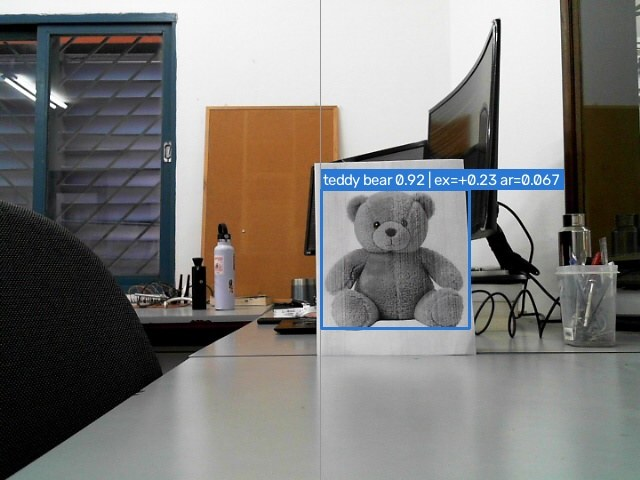
\includegraphics[width=\textwidth]{img_sana.jpg}

      {\scriptsize Sobre el escritorio: sana. El oso con confianza 0,91 en todos
      los frames.}
    \end{column}
    \begin{column}{0.32\textwidth}
      \centering
      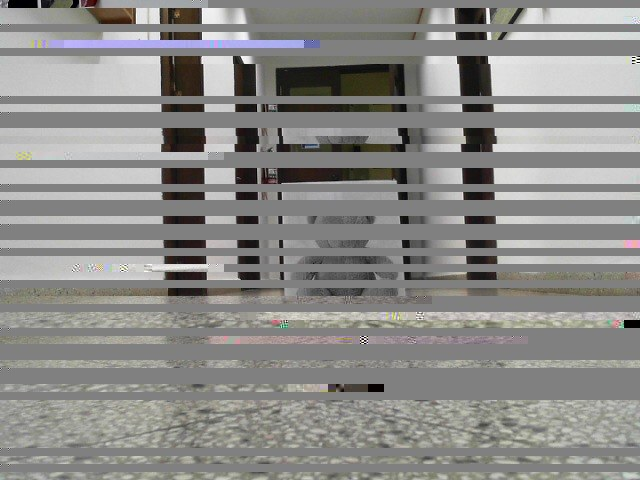
\includegraphics[width=\textwidth]{img_rota_37.jpg}

      {\scriptsize En el piso, \textbf{robot quieto y 12 V desenchufados}: 37 \% de
      las filas en franja. El oso está detrás.}
    \end{column}
    \begin{column}{0.32\textwidth}
      \centering
      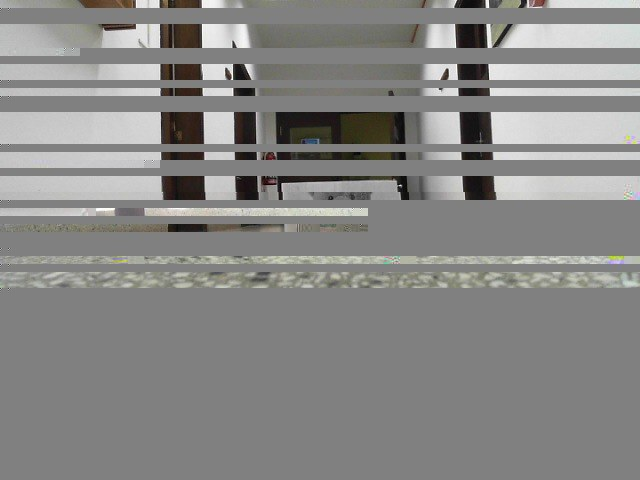
\includegraphics[width=\textwidth]{img_rota_63.jpg}

      {\scriptsize El peor frame de esa medición: 63 \% de las filas.}
    \end{column}
  \end{columns}

  \vspace{0.5em}
  \relax{\footnotesize
  \begin{columns}[T,onlytextwidth]
    \begin{column}{0.485\textwidth}
      \begin{block}{Qué son las franjas}
        Con MJPG, cuando se pierde un paquete USB falta un tramo del JPEG, y
        el decodificador rellena con gris hasta el próximo marcador de
        reinicio. El frame llega ``entero'' pero YOLO no reconoce nada detrás.
      \end{block}
    \end{column}
    \begin{column}{0.485\textwidth}
      \begin{block}{Por qué importó tanto}
        La primera corrida no vio el oso, y la explicación a la vista era el
        paso de giro. Mirar un frame quieto antes de tocar el paso evitó
        ``arreglar'' el barrido con la cámara ciega.
      \end{block}
    \end{column}
  \end{columns}}
\end{frame}

\begin{frame}{La imagen rota (2 de 2): qué se descartó y qué no}
  \begin{columns}[T,onlytextwidth]
    \begin{column}{0.40\textwidth}
      \centering
      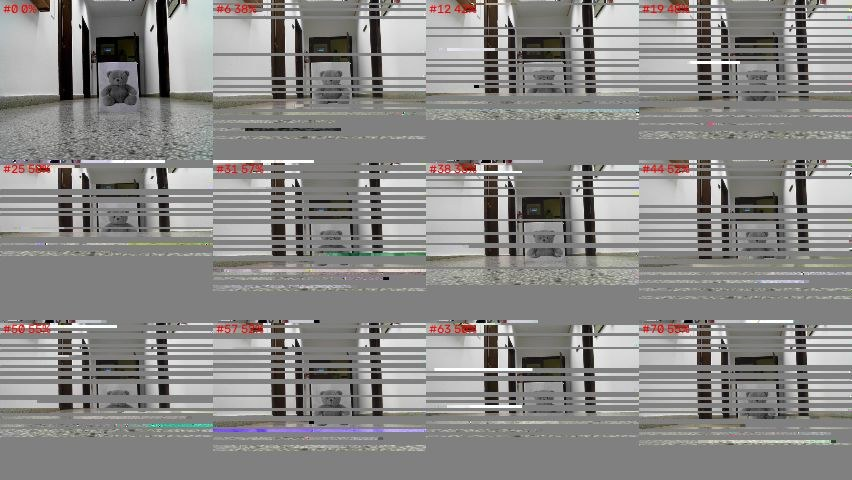
\includegraphics[width=0.80\textwidth]{grilla_rota.jpg}

      {\scriptsize 15:28 --- 69 de 71 frames rotos.}

      \vspace{0.3em}
      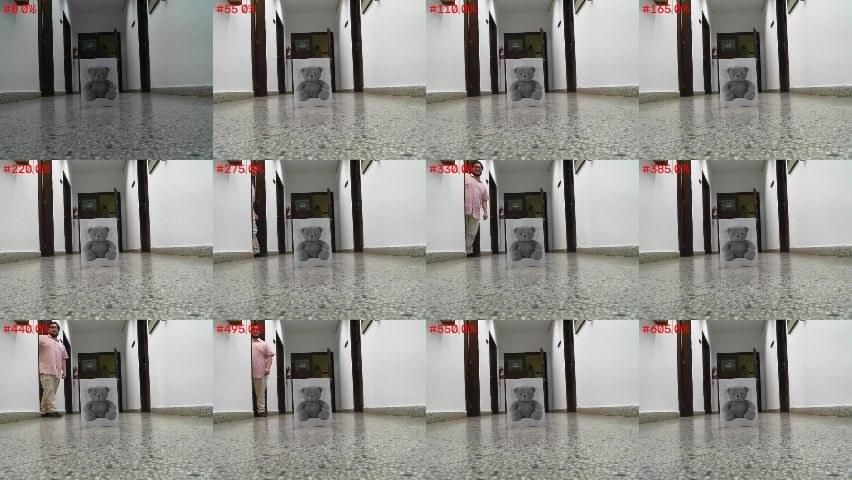
\includegraphics[width=0.80\textwidth]{grilla_limpia.jpg}

      {\scriptsize 15:52 --- 0 de 606. Nadie tocó los cables.}
    \end{column}
    \begin{column}{0.57\textwidth}
      \relax{\footnotesize
      \begin{block}{Descartado con mediciones}
        \begin{itemize}
          \item El PWM de los motores: pasa con los motores parados.
          \item La fuente de 12 V: igual con la UPS desenchufada.
          \item La carga del procesador: se rompe capturando sin YOLO.
          \item La alimentación del Pi: \cod{0x0}, 4,97 a 5,14 V.
          \item El ancho de banda USB: negocia el máximo y usa la octava parte.
          \item La cámara en sí: en los ratos buenos, 150 de 150 frames sanos.
        \end{itemize}
      \end{block}
      \begin{block}{Lo que sí se sabe}
        Son \textbf{paquetes USB perdidos}: con la traza del driver, el kernel
        registra cientos en los ratos malos y ninguno en los buenos.
      \end{block}
      \begin{alertblock}{Lo que no se sabe: la causa}
        Quedan el cable o conector de la webcam y el límite de 600 mA de los
        USB. El problema \textbf{desapareció solo} antes de poder aislarlo.
        Puede volver.
      \end{alertblock}}
    \end{column}
  \end{columns}
\end{frame}

\begin{frame}{Medir el paso de giro con la propia cámara}
  \centering
  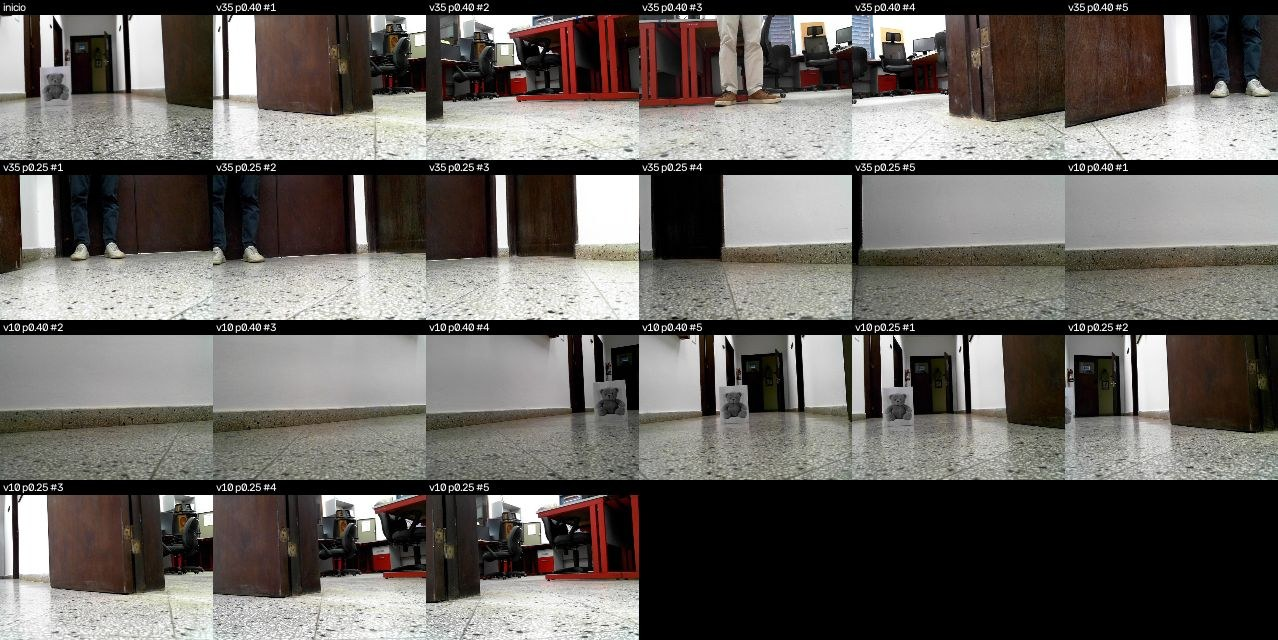
\includegraphics[width=0.55\textwidth]{paso_giro.jpg}

  \vspace{0.2em}
  \relax{\footnotesize
  \begin{columns}[T,onlytextwidth]
    \begin{column}{0.485\textwidth}
      \begin{block}{Qué muestra}
        Un frame por pausa, con el robot quieto, a lo largo de 20 pulsos de
        giro en cuatro tandas. Comparando cada frame con el anterior
        (emparejando puntos de la mitad de arriba, que es lo lejano) sale
        cuántos píxeles se corrió la escena.
      \end{block}
    \end{column}
    \begin{column}{0.485\textwidth}
      \begin{block}{Qué se sacó}
        \begin{itemize}
          \item El paso vigente renovaba el 61 \% de la imagen: demasiado.
          \item El oso reaparece en el mismo lugar tras 15 pasos y pico: una
                vuelta son $\sim$4400 px, o sea un campo visual de
                \textbf{$\sim$52\grad}.
        \end{itemize}
      \end{block}
    \end{column}
  \end{columns}}
\end{frame}

\begin{frame}{El comportamiento completo, visto desde el robot}
  \relax{\footnotesize
  \begin{columns}[c,onlytextwidth]
    \begin{column}{0.43\textwidth}
      \centering
      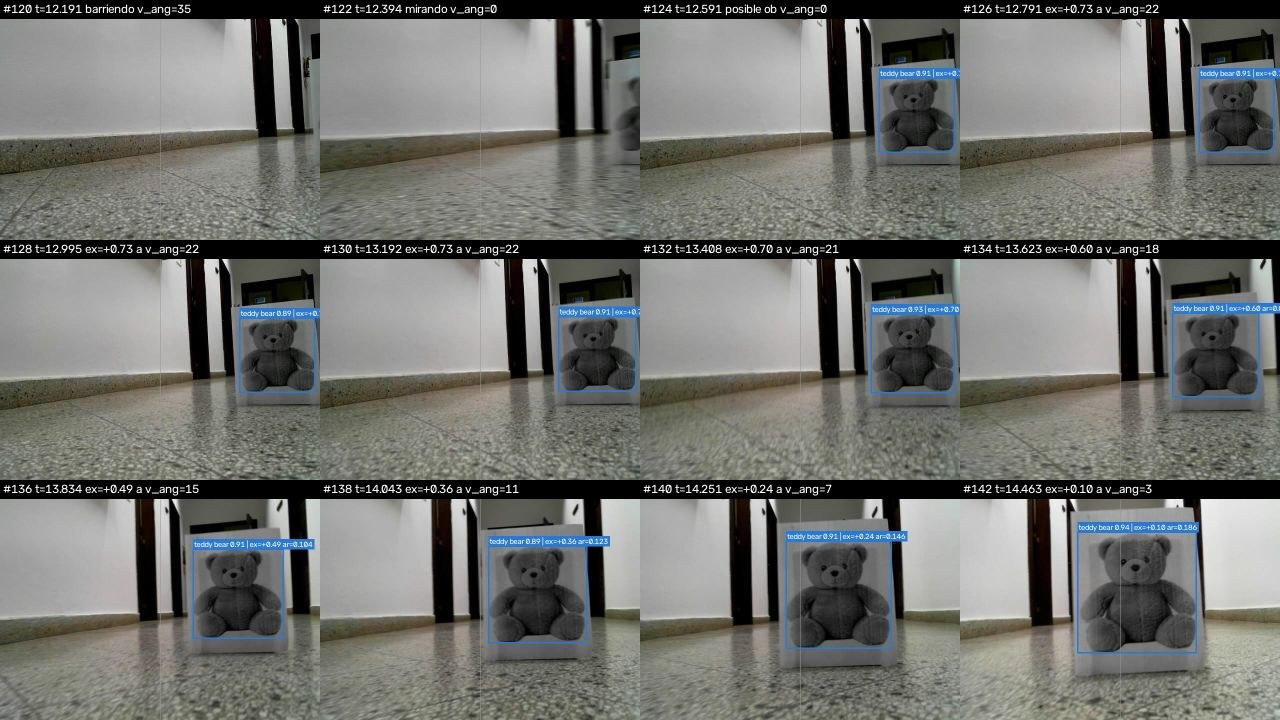
\includegraphics[width=\textwidth]{aprox_a.jpg}

      \vspace{0.2em}
      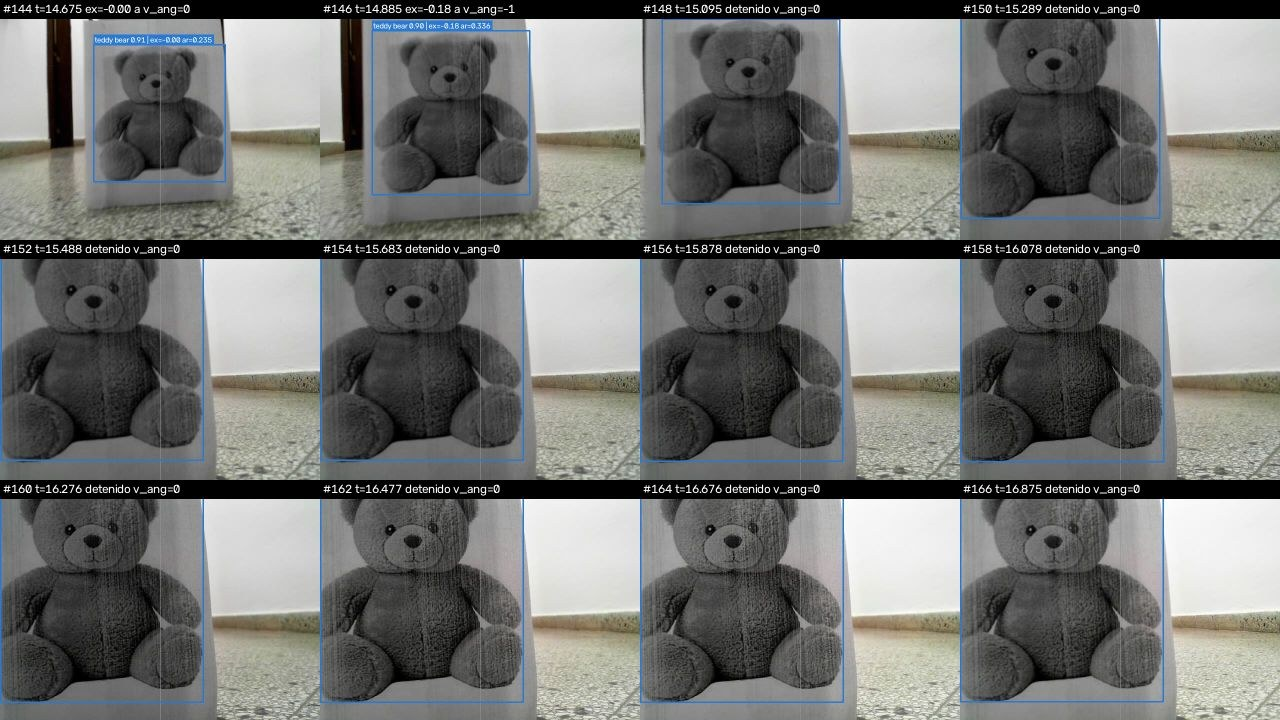
\includegraphics[width=\textwidth]{aprox_b.jpg}
    \end{column}
    \begin{column}{0.55\textwidth}
      \begin{block}{Qué se ve (corrida de las 16:29)}
        Arriba a la izquierda, el último paso del barrido. El oso entra por el
        borde derecho, el robot se queda quieto (``posible objetivo''), lo
        confirma y avanza. En las filas siguientes el oso va hacia el centro
        mientras crece, hasta que el robot frena y queda detenido.
      \end{block}
      \begin{block}{Los números de esa corrida}
        15 pasos de barrido; confirmado 0,2 s después de verlo; 2,3 s de
        aproximación; el error lateral bajó de $+0{,}73$ a cero en 2 s sin
        cruzarse de lado. Cada cuadro lleva el frame, el tiempo y el motivo
        del comando.
      \end{block}
    \end{column}
  \end{columns}}
\end{frame}

\begin{frame}{La mochila que resultó ser una valija}
  \begin{columns}[T,onlytextwidth]
    \begin{column}{0.36\textwidth}
      \centering
      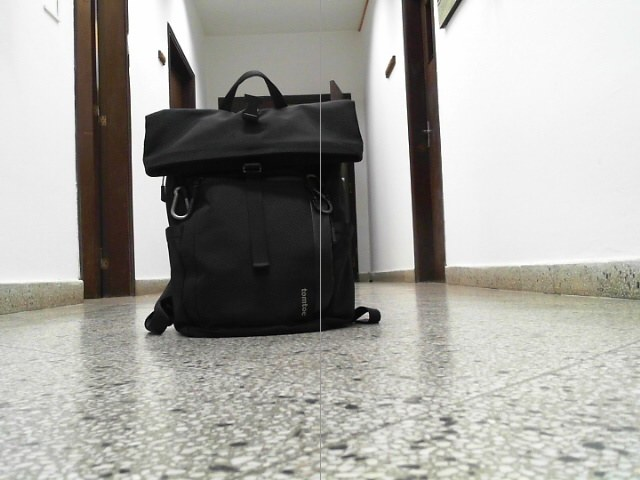
\includegraphics[width=\textwidth]{mochila.jpg}

      {\scriptsize Lo que ve el robot: la mochila a 1 m, desde el piso. Para
      YOLOv8n, \cod{suitcase} con confianza 0,60.}
    \end{column}
    \begin{column}{0.61\textwidth}
      \relax{\footnotesize
      \begin{block}{Cómo se supo}
        La cámara la veía perfecta y \cod{demo.sh ver} decía ``nada''.
        \cod{que_ve.py} le preguntó al modelo por \emph{todas} las clases:
        \cod{suitcase} en 15 de 15 frames, \cod{backpack} en ninguno.
      \end{block}
      \begin{block}{Por qué}
        El modelo aprendió mochilas colgadas de una espalda, vistas a la altura
        de una persona. Apoyada en el piso y mirada desde abajo, con la tapa
        enrollada, se parece más a una valija.
      \end{block}
      \begin{block}{Qué se hizo}
        \begin{itemize}
          \item \textbf{Alias}: \cod{suitcase} cuenta como la amenaza.
          \item \textbf{Umbral propio de 0,20}: a 1,2 m la confianza baja a
                0,32--0,41, justo en el umbral general de 0,35.
        \end{itemize}
      \end{block}
      \begin{alertblock}{El costo}
        Con 0,20, objetos oscuros grandes dan frames sueltos de falsa alarma:
        un marco de puerta, unos sillones negros. Uno solo no dispara nada
        (hacen falta 3 seguidos), pero hay que mirar el fondo de la sala.
      \end{alertblock}}
    \end{column}
  \end{columns}
\end{frame}

\begin{frame}{La huida, vista desde el robot}
  \relax{\footnotesize
  \begin{columns}[c,onlytextwidth]
    \begin{column}{0.43\textwidth}
      \centering
      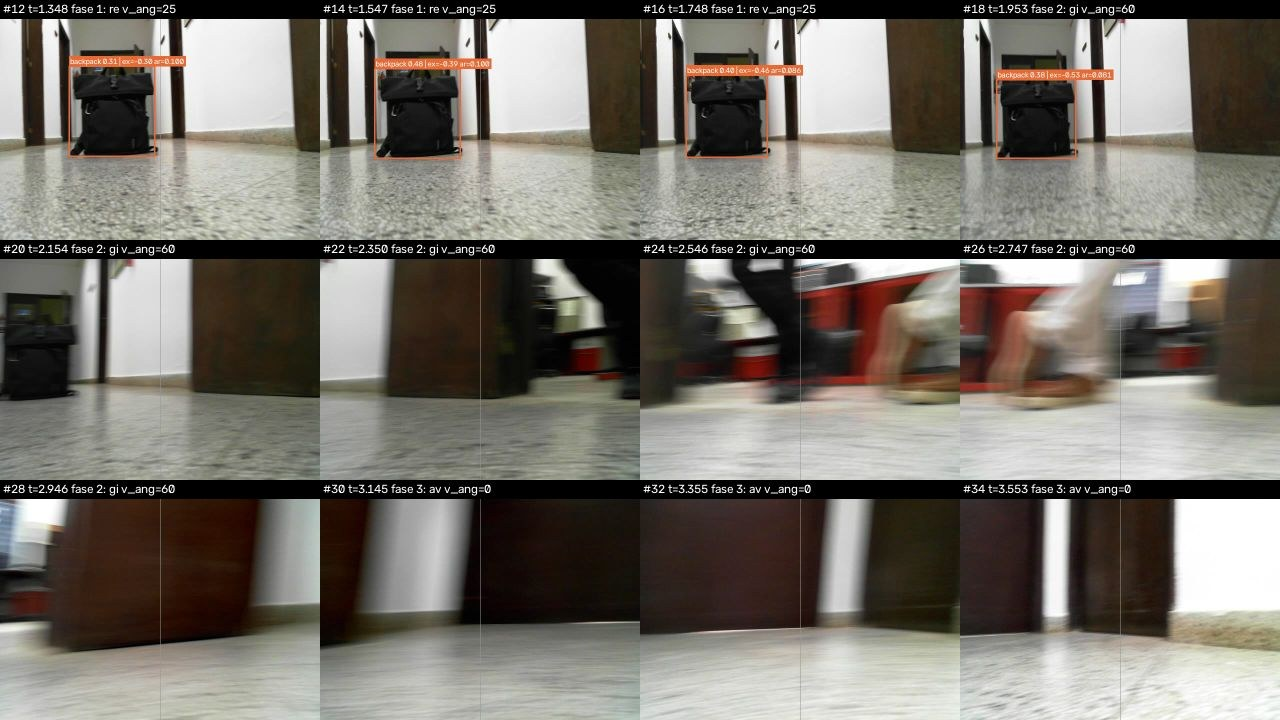
\includegraphics[width=\textwidth]{huir_a.jpg}

      \vspace{0.2em}
      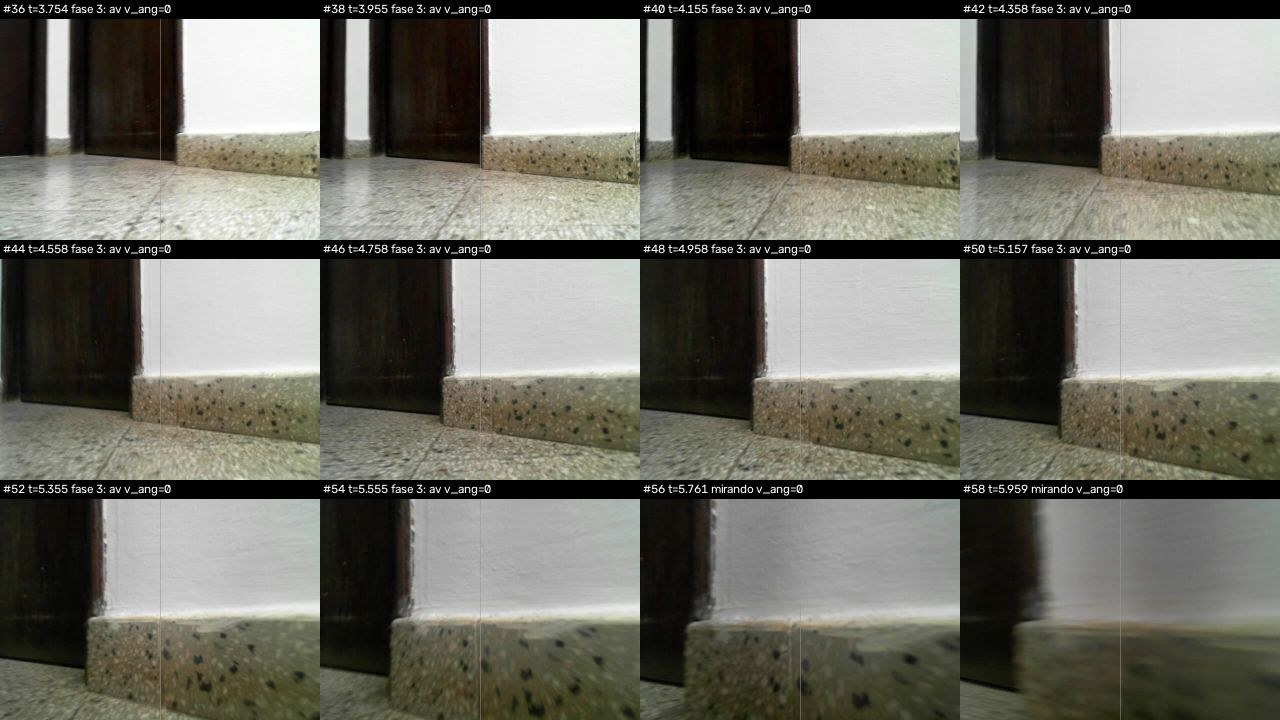
\includegraphics[width=\textwidth]{huir_b.jpg}
    \end{column}
    \begin{column}{0.55\textwidth}
      \begin{block}{Qué se ve (corrida de las 16:54)}
        Primera fila: retrocediendo, con la mochila alejándose y corriéndose
        hacia un borde (el robot gira mientras retrocede). Segunda fila: el
        giro en el lugar, con la imagen movida. De la tercera en adelante:
        avanzando, ya de espaldas, hasta quedar cerca de una pared.
      \end{block}
      \begin{block}{Los cuatro intentos}
        \begin{enumerate}
          \item No frenaba al ver la mochila sin confirmar.
          \item Confianza al borde del umbral; giraba antes de mirar.
          \item La fase 2 giraba al revés que la 1: $\sim$110\grad.
          \item Bien. Con 1,3 s se pasó de media vuelta; quedó en 1,2 s.
        \end{enumerate}
      \end{block}
    \end{column}
  \end{columns}}
\end{frame}

\begin{frame}{La demo completa (la del video)}
  \relax{\footnotesize
  \begin{columns}[c,onlytextwidth]
    \begin{column}{0.43\textwidth}
      \centering
      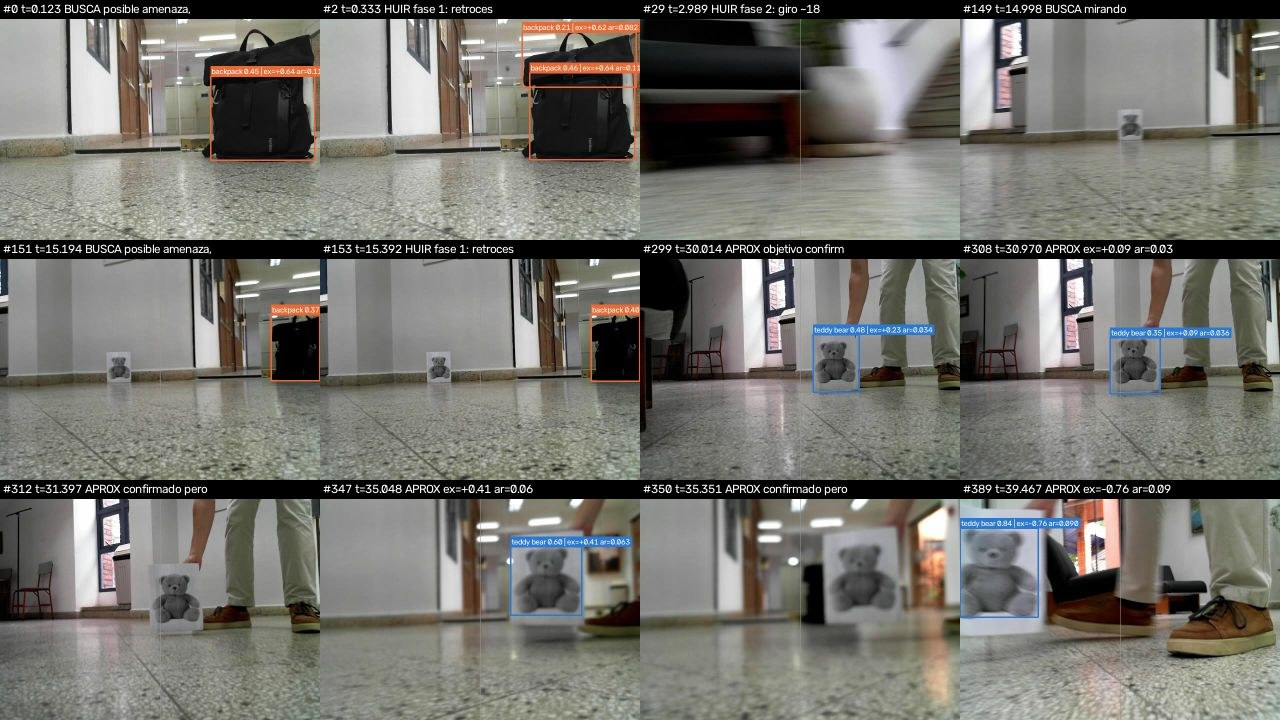
\includegraphics[width=\textwidth]{demo2_a.jpg}

      \vspace{0.2em}
      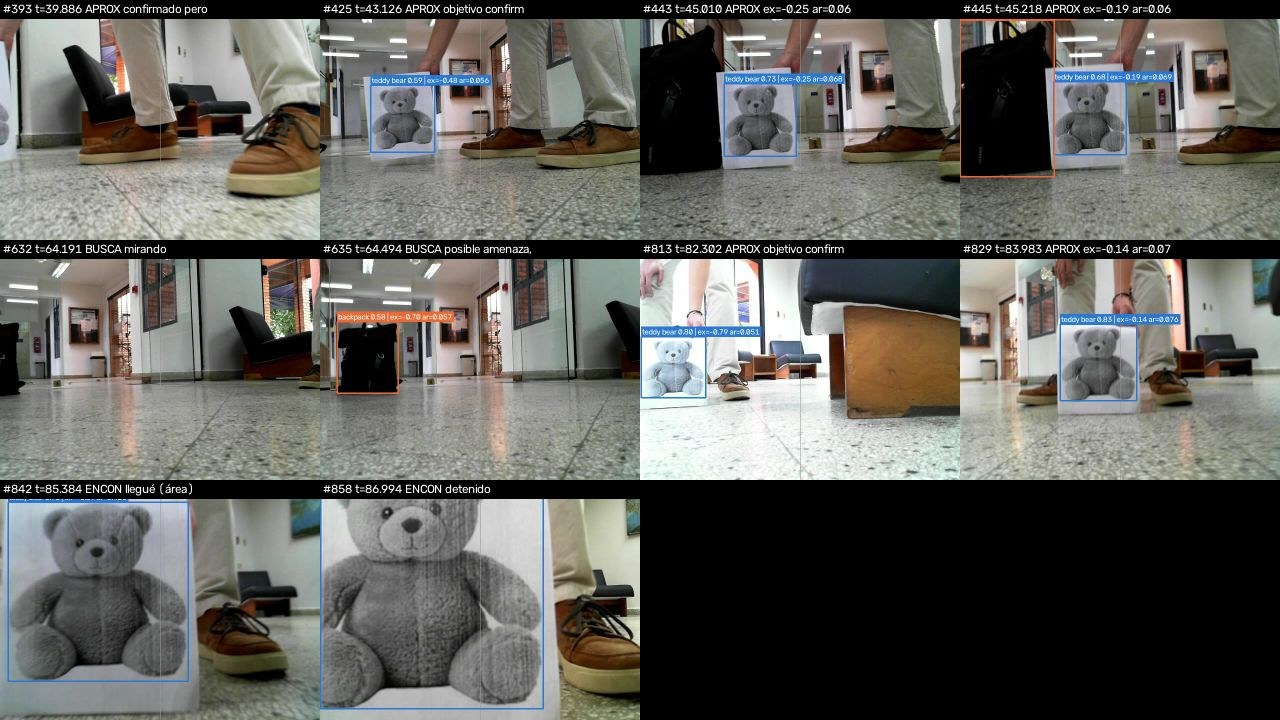
\includegraphics[width=\textwidth]{demo2_b.jpg}
    \end{column}
    \begin{column}{0.55\textwidth}
      \begin{block}{Qué se ve}
        Momentos de la corrida de 90 s, en un espacio abierto. Arriba: la
        mochila enfrente al arrancar (huye), y alguien moviendo el oso. Abajo:
        la mochila puesta junto al oso (caja naranja, cortada por el borde)
        dispara la huida aunque el robot vaya hacia el oso; después la mochila
        sola, y la llegada final.
      \end{block}
      \begin{block}{Cómo leer esa corrida}
        Las cuatro huidas fueron ante la mochila real. Las tres veces que
        ``perdió'' el oso, alguien lo estaba moviendo con la mano. Llegó a
        \cod{ENCONTRADO} a los 85 s, a unos 26 cm. El video está en
        \cod{media/}.
      \end{block}
    \end{column}
  \end{columns}}
\end{frame}

\begin{frame}{Lo que cambió ese día}
  \relax{\footnotesize
  \begin{tabular}{L{3.4cm}L{1.7cm}L{1.7cm}L{6.8cm}}
    \toprule
    \textbf{Qué} & \textbf{Antes} & \textbf{Después} & \textbf{Por qué} \\
    \midrule
    \cod{BUSCAR_PASO_GIRO_S} & 0,40 & 0,25 & El paso renovaba el 61 \% de la imagen \\
    \cod{BUSCAR_GIRO_S} & 9 & 17 & Una vuelta entera con pasos de 18\grad \\
    Orden del barrido & gira, mira & mira, gira & No apartar la vista antes de mirar \\
    Frenar al ver & sólo el oso & oso y mochila & La mochila no llegaba a confirmarse \\
    Envío de comandos & con el latido & en el acto & Los pulsos cortos salían con retardo al azar \\
    \cod{KP_ANG} & 0,8 & 0,5 & 0,8 se pasaba; 0,3 perdía el oso \\
    Giro al avanzar & sin límite & $\leq 0{,}7 \cdot v_{lin}$ & Ninguna rueda se detiene ni se invierte \\
    \cod{V_LIN_MAX} & 72 & 55 & Más tiempo para centrar \\
    \cod{AREA_OBJETIVO}, \cod{KP_LIN} & 0,222 y 4,5 & 0,35 y 2,4 & Frenar a 30 cm en vez de a 50 \\
    Clase de la mochila & \cod{backpack} & más \cod{suitcase} & Así la ve el modelo desde el piso \\
    Umbral de la mochila & 0,35 & 0,20 & A 1,2 m da 0,32--0,41 \\
    Fase 2 de \cod{HUIR} & a la derecha & como la fase 1 & Deshacía el giro del retroceso \\
    \cod{HUIR_GIRO_S} & 1,1 & 1,2 & 1,1 daba 110\grad; 1,3 se pasaba \\
    Búsqueda tras perder el oso & a la derecha & hacia donde lo vio & Tardó 23 s en reencontrarlo \\
    Registro & --- & columna \cod{franjas} & Saber si la cámara estaba ciega \\
    \bottomrule
  \end{tabular}}
\end{frame}

% =============================================================================
\section{El 2 de octubre: ultrasónico y buzzer}
% =============================================================================

\begin{frame}{El robot terminado}
  \centering
  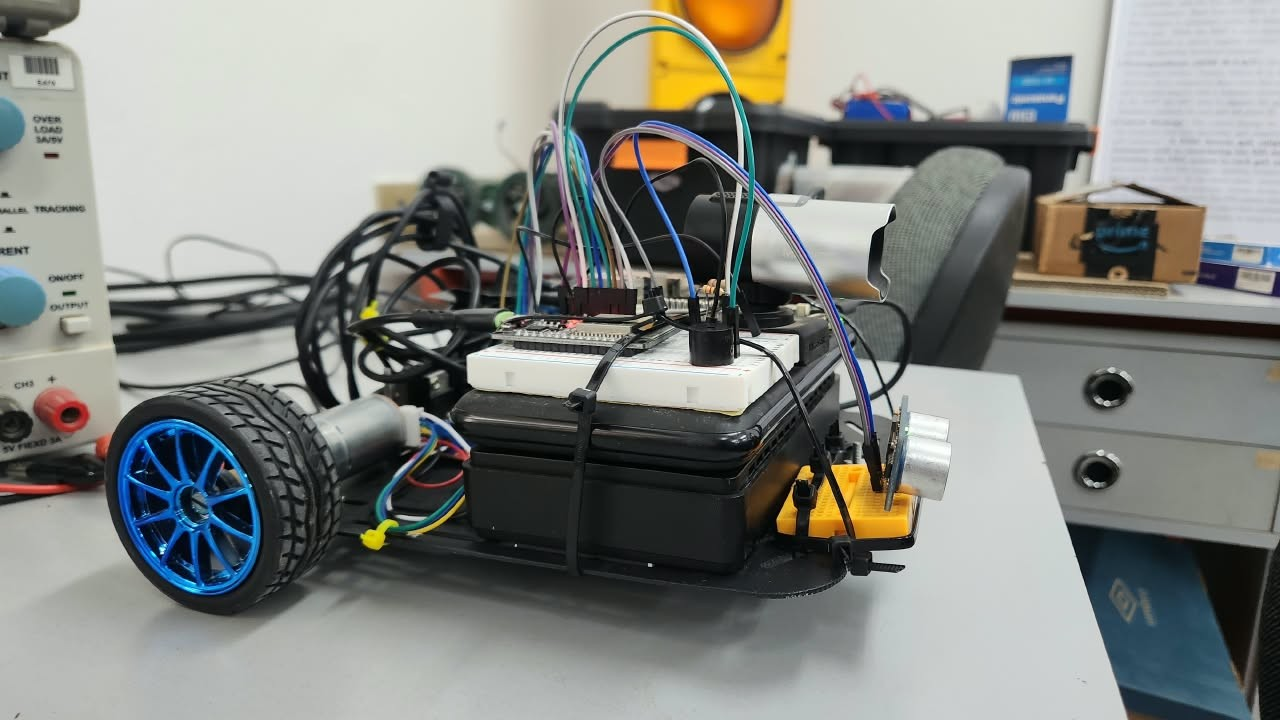
\includegraphics[height=0.37\textheight]{robot_terminado_lado.jpg}\hspace{1.5mm}%
  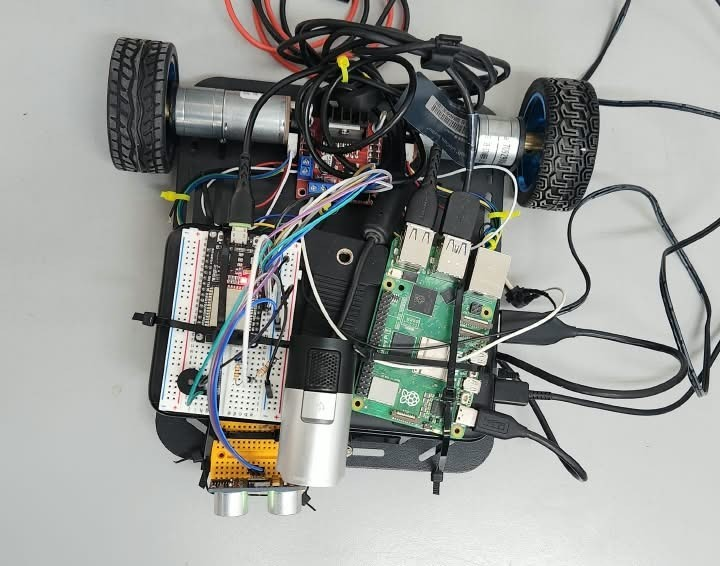
\includegraphics[height=0.37\textheight]{robot_terminado_arriba.jpg}\hspace{1.5mm}%
  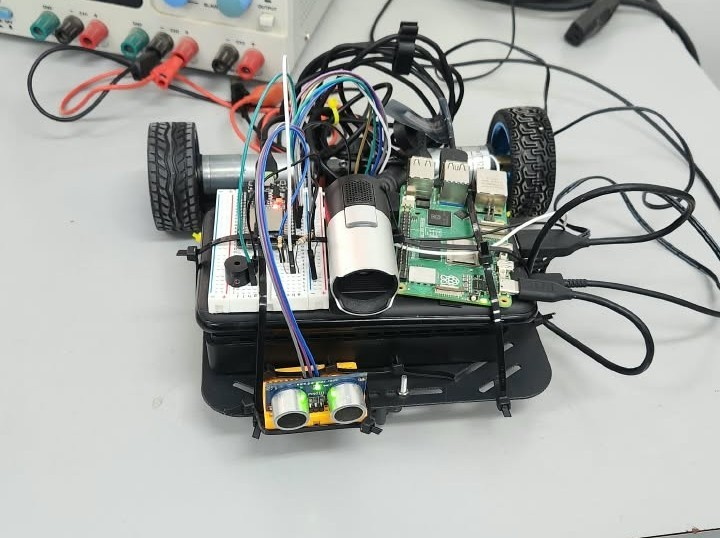
\includegraphics[height=0.37\textheight]{robot_terminado_frente.jpg}

  \vspace{0.3em}
  \relax{\footnotesize
  \begin{columns}[T,onlytextwidth]
    \begin{column}{0.485\textwidth}
      \begin{block}{Qué se ve}
        \begin{itemize}
          \item Al frente, sobre una protoboard amarilla, el \textbf{ultrasónico}
                (los dos ``ojos''), y arriba la \textbf{webcam}.
          \item En la protoboard blanca, el \textbf{ESP32}, el divisor del
                sensor y el \textbf{buzzer} (el cilindro negro).
          \item Al lado, la \textbf{Raspberry Pi 5}; atrás, el \textbf{L298N}
                (rojo) y los dos motores.
          \item Debajo, la caja negra con las baterías.
        \end{itemize}
      \end{block}
    \end{column}
    \begin{column}{0.485\textwidth}
      \begin{block}{Qué cambió respecto del 1 de octubre}
        El día anterior se había decidido dejar el ultrasónico y el buzzer para
        una segunda versión, por tiempo. El 2 de octubre se \textbf{revirtió}:
        la idea era agregar el ultrasónico ``en media hora'', para que el robot
        no chocara contra las paredes al huir.
      \end{block}
      \begin{alertblock}{Lo que llevó}
        Algo más de \textbf{dos horas}, y entró también el buzzer. Las fotos
        están en \cod{Fotos del bot/}.
      \end{alertblock}
    \end{column}
  \end{columns}}
\end{frame}

\begin{frame}{Cómo quedó cableado}
  \begin{columns}[T,onlytextwidth]
    \begin{column}{0.50\textwidth}
      \relax{\footnotesize
      \begin{tabular}{L{2.1cm}L{0.9cm}L{3.2cm}}
        \toprule
        \textbf{Señal} & \textbf{GPIO} & \textbf{Nota} \\
        \midrule
        PING))) \textbf{SIG} & \textbf{12} & Con divisor. Disparo y eco por el mismo pin \\[1pt]
        PING))) \textbf{5V} & VIN & 5 V del USB \\[1pt]
        PING))) \textbf{GND} & GND & Común con el ESP32 \\[1pt]
        Buzzer \textbf{+} & \textbf{14} & Activo, de dos patas, directo \\[1pt]
        Buzzer \textbf{--} & GND & \\
        \bottomrule
      \end{tabular}}

      \vspace{0.2em}
      \centering
      \begin{tikzpicture}[font=\footnotesize]
        \node (sig) at (0,0) {SIG};
        \node[draw, minimum width=1.1cm, minimum height=0.36cm] (r1) at (1.6,0) {1 k$\Omega$};
        \coordinate (n) at (3.0,0);
        \node (gpio) at (4.5,0) {GPIO 12};
        \node[draw, minimum width=0.9cm, minimum height=0.36cm] (r2) at (3.0,-0.85) {2 k$\Omega$};
        \node (gnd) at (3.0,-1.65) {GND};
        \draw (sig) -- (r1) -- (n) -- (gpio);
        \fill (n) circle (1.4pt);
        \draw (n) -- (r2) -- (gnd);
      \end{tikzpicture}
    \end{column}
    \begin{column}{0.47\textwidth}
      \relax{\footnotesize
      \begin{block}{Por qué el divisor}
        El sensor contesta a \textbf{5 V} y el ESP32 no los tolera. Hacia el
        ESP32 baja a 3,3 V; hacia el sensor, el disparo llega a 3,3 V por la
        de 1 k$\Omega$, que alcanza (la entrada es TTL).
        \ojo{Cruzadas}, el eco llega a 1,7 V y el sensor parece mudo.
      \end{block}
      \begin{block}{Por qué esos pines}
        El plan era el 19 para el sensor y el 4 para el buzzer. En la
        protoboard sólo queda accesible \textbf{una fila} del ESP32, y de esa
        fila los únicos libres que pueden ser salida son el 12 y el 14.
      \end{block}
      \begin{alertblock}{Dos trampas de pines}
        \begin{itemize}
          \item El \textbf{35} es de sólo entrada: el buzzer se conectó ahí
                primero, y ahí no suena.
          \item El \textbf{12} es pin de arranque: en alto al salir del reset,
                el ESP32 no arranca. La de 2 k$\Omega$ lo tiene en bajo.
        \end{itemize}
      \end{alertblock}}
    \end{column}
  \end{columns}
\end{frame}

\begin{frame}{El firmware: un sensor de un solo pin}
  \relax{\footnotesize
  \begin{columns}[T,onlytextwidth]
    \begin{column}{0.485\textwidth}
      \begin{block}{Qué había y qué hizo falta}
        El firmware estaba escrito para un HC-SR04, con un pin para disparar y
        otro para el eco. El \textbf{Parallax PING)))} usa uno solo: el ESP32
        manda el pulso de disparo y enseguida escucha por el mismo cable.
      \end{block}
      \begin{block}{Cómo se hace}
        \begin{enumerate}
          \item El pin pasa a \textbf{salida} y da un pulso de 5 $\mu$s.
          \item Pasa a \textbf{entrada}. El sensor espera 750 $\mu$s antes de
                contestar: sobra tiempo.
          \item Una interrupción mide el ancho del pulso de eco: 58 $\mu$s por
                centímetro.
        \end{enumerate}
        La interrupción sólo mira dentro de la \textbf{ventana de escucha}:
        así el propio disparo nunca se toma por un eco.
      \end{block}
    \end{column}
    \begin{column}{0.485\textwidth}
      \begin{block}{Lo que hay que saber de las lecturas}
        \begin{itemize}
          \item \textbf{$\sim$370 cm es ``libre''}: sin nada adelante el sensor
                devuelve su pulso más largo. No es una distancia.
          \item \textbf{$-1$ es ``no contestó''}: sensor desconectado. El Pi lo
                lee como ``no sé'', no como distancia cero.
          \item Mide de 2 cm a 3 m, cada 60 ms.
        \end{itemize}
      \end{block}
      \begin{block}{Lo que quedó en el firmware}
        \begin{itemize}
          \item \cod{PIN_SONAR} 12, \cod{PIN_BUZZER} 14, \cod{BUZZER_PASSIVE} 0.
          \item Tecla \cod{e}: contadores del sensor (disparos, flancos, ecos).
          \item Tecla \cod{u}: un disparo y la línea mirada con el ADC.
          \item Tecla \cod{U}: línea en alto fijo, para medirla con el tester.
        \end{itemize}
      \end{block}
    \end{column}
  \end{columns}}
\end{frame}

\begin{frame}{El primer sensor estaba muerto: cómo se descartó todo lo demás}
  \relax{\footnotesize
  \begin{tabular}{L{6.2cm}L{7.4cm}}
    \toprule
    \textbf{Prueba} & \textbf{Qué descartó} \\
    \midrule
    Contadores de disparos, entradas a la interrupción y ecos &
      La interrupción: ve exactamente 2 flancos por disparo, los del propio
      pulso \\[1pt]
    Leer el pin con el pull-up interno puesto &
      Que el divisor no estuviera en ese pin: lee 0, hay camino a GND \\[1pt]
    La línea mirada con el ADC durante 25 ms después del disparo &
      Un eco a media altura por las resistencias cruzadas: 0,00 V \\[1pt]
    Disparos de 5, 20, 100 y 1000 $\mu$s &
      El ancho del disparo \\[1pt]
    Línea en alto fijo, medida con el tester sobre los pines del sensor &
      El cableado: 3,3 V en SIG y 5 V en la alimentación \\
    \bottomrule
  \end{tabular}}

  \vspace{0.5em}
  \relax{\footnotesize
  \begin{columns}[T,onlytextwidth]
    \begin{column}{0.485\textwidth}
      \begin{block}{El resultado}
        Con todo eso bien, el sensor seguía mudo. Cambiado por otro igual:
        \textbf{30 cm clavados, 120 de 120 lecturas}, con una caja a 30 cm.
        Costó unos 20 minutos.
      \end{block}
    \end{column}
    \begin{column}{0.485\textwidth}
      \begin{block}{Por qué se hizo así}
        Con todas las lecturas en $-1$ no se sabe si falla el firmware, el
        cableado o el sensor. Cada prueba se agregó al firmware para descartar
        una causa \textbf{sin pedirle al usuario que revisara a ciegas}. El
        procedimiento quedó en el \cod{RUNBOOK.md}, Paso 25.
      \end{block}
    \end{column}
  \end{columns}}
\end{frame}

\begin{frame}{Cómo usa el Pi la distancia}
  \relax{\footnotesize
  \begin{columns}[T,onlytextwidth]
    \begin{column}{0.485\textwidth}
      \begin{block}{Dos umbrales}
        \begin{itemize}
          \item \cod{DIST_PARADA_CM} = \textbf{20}: el de \emph{llegada}. En
                \cod{APROXIMAR}, algo a menos de 20 cm cuenta como llegada si es
                el oso; si no, se desvía.
          \item \cod{DIST_OBSTACULO_CM} = \textbf{30}: el de \emph{esquivar}. En
                la fase 3 de \cod{HUIR} y en el pulso de avance de
                \cod{BUSCAR}: no avanza, \textbf{gira en el lugar}.
        \end{itemize}
        Al oso hay que poder acercarse; a una pared, no.
      \end{block}
      \begin{block}{Retención: 0,3 s}
        Un obstáculo se da por cierto hasta 0,3 s después de la última lectura
        que lo vio (\cod{SONAR_RETENCION_S}). Girando frente a una pared el eco
        se pierde de a ratos y aparece un ``libre'' falso.
      \end{block}
    \end{column}
    \begin{column}{0.485\textwidth}
      \begin{block}{¿El eco es el oso?}
        Si el oso está a la vista con $|error_x| < 0{,}7$ y ya ocupa el 60 \%
        del área objetivo, lo que hay adelante es él. El 0,7 sale del cono del
        sensor ($\pm$20\grad) contra el semicampo de la cámara (26\grad).
      \end{block}
      \begin{alertblock}{Lo que el sensor no arregla}
        \begin{itemize}
          \item \textbf{Sólo mira adelante.} El retroceso y el giro de la huida
                siguen a ciegas: las lecturas más bajas del día (7 y 13 cm)
                fueron al terminar el giro, no avanzando.
          \item \textbf{Una pared muy de costado no la ve} hasta estar encima:
                el eco rebota para otro lado.
          \item \textbf{Sin lectura, el robot anda igual pero a ciegas.}
                \cod{main.py} lo avisa al arrancar.
        \end{itemize}
      \end{alertblock}
    \end{column}
  \end{columns}}
\end{frame}

\begin{frame}{El día, prueba por prueba}
  \relax{\footnotesize
  \begin{tabular}{L{1.1cm}L{3.6cm}L{8.9cm}}
    \toprule
    \textbf{Dónde} & \textbf{Prueba} & \textbf{Qué pasó} \\
    \midrule
    banco & Primer sensor & Todas las lecturas en $-1$. Cinco pruebas después:
      el sensor está muerto. \\[1pt]
    banco & Segundo sensor & 30 cm con una caja a 30 cm, 120 de 120. \\[1pt]
    piso & Quieto, pared a 1,5 m & 153 cm, estable. Sin ecos del piso. \\[1pt]
    piso & Avance hasta leer 20 cm & A velocidad 40: manda frenar leyendo 19 y
      queda a \textbf{16 cm}. \\[1pt]
    10:34 & Huida, pared a 1 m & El avance terminó solo a 27 cm: el sensor no
      llegó a actuar. \\[1pt]
    10:36 & Huida, pared a 80 cm & \textbf{Esquiva}: corta a 18 cm y gira.
      Después lee 16, \textbf{150}, 11 y avanza un ciclo. \\[1pt]
    10:41 & Demo del oso & Se acerca sin desvíos falsos (119 a 28 cm) y frena
      por tamaño. \\[1pt]
    10:54 & (cable del sensor suelto) & \ojo{553 filas sin lectura}: 52 s a
      ciegas, cortada a mano. \\[1pt]
    10:59 & Con dos umbrales y buzzer & Corta el avance a \textbf{29 cm}; no
      baja de 27. Suena en los tres momentos. \\[1pt]
    11:07 & Grabada (la del video) & Huye a los 2 s, esquiva a 29 cm, encuentra
      el oso a los 8 s. \\
    \bottomrule
  \end{tabular}}

  \vspace{0.3em}
  {\footnotesize Seis corridas con el programa completo, \textbf{3675 frames y
  ninguno con franjas}. Al mediodía: 69 verificaciones (eran 60); a la tarde, 79.}
\end{frame}

\begin{frame}{Tres ajustes, cada uno por una corrida}
  \relax{\footnotesize
  \begin{columns}[T,onlytextwidth]
    \begin{column}{0.32\textwidth}
      \begin{block}{1. El oso descentrado}
        Al llegar, oso grande pero corrido a la derecha ($+0{,}53$) y el sensor
        en 22 cm. Con 20 lo habría tomado por un obstáculo ajeno y habría
        girado a tope para el otro lado.

        \vspace{0.3em}
        \cod{SONAR_CENTRADO}: \textbf{0,35 \hacia{} 0,7}. La regla pedía un oso
        más centrado de lo que el sensor distingue.
      \end{block}
    \end{column}
    \begin{column}{0.32\textwidth}
      \begin{block}{2. La lectura suelta}
        Girando frente a la pared: 16 cm, \textbf{150}, 11. Con el 150 avanzó
        un ciclo contra la pared.

        \vspace{0.3em}
        \cod{SONAR_RETENCION_S} = \textbf{0,3}. En la corrida siguiente apareció
        un 172 entre lecturas de 12--16 y el robot no avanzó.
      \end{block}
    \end{column}
    \begin{column}{0.32\textwidth}
      \begin{block}{3. Poco margen}
        Con un solo umbral de 20 cm, en las huidas la lectura bajó a 16, 11 y
        12 cm: el robot no frena, pivotea, y el frente barre un arco.

        \vspace{0.3em}
        \cod{DIST_OBSTACULO_CM} = \textbf{30}, aparte del de llegada. Corta a
        29 y no baja de 27.
      \end{block}
    \end{column}
  \end{columns}}

  \vspace{0.6em}
  \begin{alertblock}{Los tres valen por una sola corrida}
    \footnotesize Son ajustes a ojo, hechos sobre lo que mostró el registro.
    Ninguno tiene una serie de mediciones detrás.
  \end{alertblock}
\end{frame}

\begin{frame}{Lo que falló ese día, fuera del sensor}
  \relax{\footnotesize
  \begin{columns}[T,onlytextwidth]
    \begin{column}{0.485\textwidth}
      \begin{block}{El estreno de los comandos de la noche anterior}
        \begin{itemize}
          \item \cod{demo.sh correr}, con la webcam desenchufada, mostraba el
                análisis de la corrida \textbf{del día anterior} como si fuera
                el de ésta. Ahora dice que no se hizo.
          \item \cod{traer_corrida.ps1} no copiaba nada: la ruta tiene
                espacios y terminaba en barra invertida. Y elegía el
                \cod{.avi} en vez del \cod{.mp4}.
          \item \cod{demo.sh firmware}, en su primer uso tras encender:
                ``comando desconocido''.
        \end{itemize}
        Los tres corregidos. El \cod{hotspot} se cargó y se probó al cierre:
        el Pi arranca en él. Sin estrenar: \cod{fondo}.
      \end{block}
      \begin{block}{Una corrida a ciegas}
        Se soltó un cable del sensor y nadie lo supo hasta ver el robot. Y al
        cancelar desde la PC, \textbf{el programa siguió andando en el Pi}.
        Quedaron el aviso de \cod{main.py} al arrancar y \cod{demo.sh sonar}.
      \end{block}
    \end{column}
    \begin{column}{0.485\textwidth}
      \begin{alertblock}{Bajo voltaje con las baterías cargándose}
        Con las baterías enchufadas a sus cargadores, el Pi marcó bajo voltaje
        en reposo: 4,72--4,80 V. Desconectadas: 5,10 V y \cod{0x0}. Visto dos
        veces el mismo día.
      \end{alertblock}
      \begin{alertblock}{La webcam se había soltado}
        Al bajar el robot al piso, el Pi dejó de verla. Reinsertada: cero
        franjas en 3675 frames.
      \end{alertblock}
      \begin{block}{Qué dice eso de la imagen rota del 1 de octubre}
        Que la causa puede haber sido el enchufe o la alimentación. Pero ese
        día cambiaron \textbf{las dos cosas a la vez}, así que no se sabe cuál.
        Sigue sin aislar.
      \end{block}
    \end{column}
  \end{columns}}
\end{frame}

\begin{frame}{Lo que cambió ese día}
  \relax{\footnotesize
  \begin{tabular}{L{3.6cm}L{2.2cm}L{2.5cm}L{5.3cm}}
    \toprule
    \textbf{Qué} & \textbf{Antes} & \textbf{Después} & \textbf{Por qué} \\
    \midrule
    Ultrasónico & sin cablear & PING))) en el GPIO 12 & Que no avance contra una pared \\
    Buzzer & sin cablear & activo, en el GPIO 14 & Avisar la huida y la llegada \\
    Firmware, sensor & HC-SR04, 2 pines & un solo pin & El sensor que había \\
    \cod{BUZZER_PASSIVE} & 1 & 0 & El buzzer es activo \\
    Pulso de avance de \cod{BUSCAR} & avanza siempre & gira si hay algo & Era el único avance sin mirar \\
    \cod{DIST_OBSTACULO_CM} & --- & 30 & Con 20, la lectura bajaba a 11 cm \\
    \cod{SONAR_RETENCION_S} & --- & 0,3 & Una lectura libre suelta hacía avanzar \\
    \cod{SONAR_CENTRADO} & 0,35 & 0,7 & El robot llega descentrado \\
    \cod{main.py} & --- & avisa si no hay lectura & Una corrida entera salió a ciegas \\
    \cod{demo.sh} & 12 comandos & 13: \cod{sonar} & Ver el sensor sin mover el robot \\
    Scripts de \cod{piso/} & --- & \cod{sonar.py}, \cod{freno_sonar.py} & Medir quieto, y dónde queda al frenar \\
    Barrido después de huir & siempre a la derecha & sorteado, o lejos de la mochila & Huía en ciclo: seis veces en un minuto \\
    Verificaciones & 60 & 79 & Los casos nuevos del sensor y del barrido \\
    \bottomrule
  \end{tabular}}

  \vspace{0.4em}
  {\footnotesize El detalle está en \cod{PLAN.md} §13, Día 15, y en
  \cod{HARDWARE.md} §9.}
\end{frame}

% =============================================================================
\section{Operación, estado y pendientes}
% =============================================================================

\begin{frame}{Cómo se opera, en siete pasos}
  \begin{enumerate}
    \item \textbf{Armar.} Cargador \hacia{} Pi por \textbf{USB-A}, sin
          enchufar a la pared. Webcam \textbf{firme} en el USB azul de abajo,
          ESP32 en el negro de abajo. UPS de 12 V \textbf{desenchufada}.
          Notebook y Pi en el mismo hotspot.
    \item \textbf{Entrar.} Desde PowerShell, en la carpeta del proyecto:
          \texttt{.\textbackslash scripts\_pi\textbackslash entrar.cmd} (busca
          el Pi y abre la sesión).
    \item \textbf{Chequear.} \cod{bash ~/TPF/scripts_pi/demo.sh chequeo}: tiene
          que terminar en \textbf{LISTO}.
    \item \textbf{Medir la imagen y el sensor.} \cod{demo.sh imagen}:
          \textbf{imagen SANA}. \cod{demo.sh sonar}: una distancia creíble, no
          \textbf{SIN LECTURA}.
    \item \textbf{Mirar.} \cod{demo.sh ver} con el oso a 1 m: \cod{teddy bear}.
          Con la mochila: \cod{backpack}. Y \cod{demo.sh fondo} sin ninguno.
    \item \textbf{Correr.} Enchufar los 12 V, robot en el piso, y
          \cod{demo.sh correr 60 "nota"} (o \cod{grabar}, con video). Tarda 10
          a 15 s en arrancar; durante la cuenta, sacar las manos.
    \item \textbf{Parar.} Ctrl+C. Emergencia: sacar los 12 V, no el Pi.
  \end{enumerate}

  \vspace{0.3em}
  \begin{columns}[T,onlytextwidth]
    \begin{column}{0.485\textwidth}
      \begin{block}{Al terminar}
        {\footnotesize Sacar los 12 V, traer el video con
        \cod{traer_corrida.cmd -Video}, \cod{demo.sh apagar}, y esperar a que
        el LED verde deje de parpadear.}
      \end{block}
    \end{column}
    \begin{column}{0.485\textwidth}
      \begin{block}{El manual para hacerlo sin ayuda}
        {\footnotesize \cod{GUIA_PRESENTACION.md} y su PDF (12 páginas): cada paso
        con lo que tiene que salir, cómo leer la pantalla, problemas, ajustes
        con vuelta atrás y plan B.}
      \end{block}
    \end{column}
  \end{columns}
\end{frame}

\begin{frame}[fragile]{Conectarse al Pi y trabajar con él}
\begin{columns}[T,onlytextwidth]
\begin{column}{0.56\textwidth}
\scriptsize
\textbf{Entrar}
\begin{verbatim}
.\scripts_pi\entrar.cmd                  # lo busca y entra
.\scripts_pi\entrar.cmd -Ip 192.168.43.57      # con la IP
ssh -i ~/.ssh/id_ed25519_pi admin@IP     # a mano
\end{verbatim}
\textbf{Copiar cambios de la PC al Pi, y traer resultados}
\begin{verbatim}
.\scripts_pi\provisionar_pi.cmd          # copia y verifica alla
.\scripts_pi\traer_corrida.cmd -Video    # registros y video
\end{verbatim}
\textbf{En el Pi, a mano}
\begin{verbatim}
cd ~/TPF/src && source ../.venv/bin/activate
python prueba_estados.py                 # las 60, todas "ok"
python main.py --simular --espera 0 --duracion 10
python analizar_corrida.py ../logs/corrida_*.csv
\end{verbatim}
\textbf{Una corrida de prueba con video y voltaje}
\begin{verbatim}
cd ~/TPF/scripts_pi/piso
GRABAR=1 bash corrida_piso.sh etiqueta 30 "nota" KP_ANG=0.4
\end{verbatim}
\end{column}
\begin{column}{0.42\textwidth}
\footnotesize
\begin{block}{El ciclo de trabajo}
  \begin{enumerate}
    \item Editar en la PC.
    \item Correr \verb|prueba_estados.py| en la PC.
    \item Copiar al Pi y correrla allá.
    \item Comparar que el código sea el mismo en los dos lados.
    \item Probar sin motores (\verb|--simular|, \verb|demo.sh ver|).
    \item Recién entonces, la corrida.
  \end{enumerate}
\end{block}
\begin{alertblock}{La red}
  En la sala no va a estar la WiFi de siempre. Hay que \textbf{cargar el
  hotspot del celular en el Pi} antes, con \verb|demo.sh hotspot|: sin eso no
  hay forma de entrar. Pendiente.
\end{alertblock}
\end{column}
\end{columns}
\end{frame}

\begin{frame}{Estado, bloque por bloque}
  \relax{\footnotesize
  \begin{tabular}{L{0.4cm}L{4.3cm}L{9.0cm}}
    \toprule
    & \textbf{Bloque} & \textbf{Estado al 2 de octubre} \\
    \midrule
    \listo & Mecánica, cableado, driver & Hecho y verificado \\
    \listo & Firmware del ESP32 & Verificado; calibración de piso, ultrasónico de un pin y buzzer \\
    \listo & Tracción & Avanza derecho y gira; rango 0,091 a 0,380 m/s \\
    \listo & Alimentación portátil & Dos fuentes; \cod{0x0} en todas las corridas \\
    \listo & Raspberry Pi y entorno & Funcionando; 12 GB libres \\
    \curso & Visión & 10,6 FPS y detecta. La imagen rota no volvió el 2/10; \ojo{causa sin aislar} \\
    \listo & Máquina de estados y control & Funcionando en el piso; 79 verificaciones \\
    \curso & Pruebas integradas & Demo hecha, con video. Faltan las 10 corridas por escenario \\
    \curso & Operación & Guía para operar sin asistencia; hotspot cargado y probado; casi todos los comandos ya corrieron en el robot. \ojo{Falta el ensayo} \\
    \listo & Ultrasónico y buzzer & Cableados y probados en el piso el 2 de octubre \\
    \pend & Encoders & Fuera del alcance: segunda versión \\
    \pend & Informe & Sin empezar. Material: la bitácora, el cuaderno, este documento \\
    \bottomrule
  \end{tabular}}

  \vspace{0.5em}
  {\footnotesize \listo{} hecho \quad \curso{} funciona, con algo pendiente
  \quad \pend{} sin hacer}
\end{frame}

\begin{frame}{Lo que falta, en orden}
  \relax{\footnotesize
  \begin{columns}[T,onlytextwidth]
    \begin{column}{0.485\textwidth}
      \begin{alertblock}{Antes de la presentación}
        \begin{enumerate}
          \item \textbf{Ensayar con la guía}, sin ayuda, por el hotspot (ya
                cargado y probado: el Pi arranca en él). Ahí se estrena
                \cod{fondo}.
          \item \textbf{Antes de cada corrida}: baterías fuera del cargador,
                webcam firme, y \cod{demo.sh sonar}.
          \item \textbf{La imagen rota}: si vuelve, Paso 24 del \cod{RUNBOOK}.
          \item En la sala: \cod{demo.sh fondo}, por las falsas alarmas, y
                decidir dónde va la mochila.
        \end{enumerate}
      \end{alertblock}
    \end{column}
    \begin{column}{0.485\textwidth}
      \begin{block}{Para el informe}
        \begin{enumerate}\setcounter{enumi}{6}
          \item \textbf{Las 10 corridas por escenario} (Paso 23 del
                \cod{RUNBOOK}): aproximación, huida, conflicto y sala vacía.
          \item \textbf{Autonomía} del cargador.
          \item Un \textbf{video desde afuera}, con sonido. Las fotos ya están.
          \item Escribirlo. El hilo conductor ya tiene veintiún casos.
        \end{enumerate}
      \end{block}
      \begin{block}{Ajustes finos que quedaron a ojo}
        \begin{itemize}
          \item Los tres del ultrasónico: una corrida cada uno.
          \item El giro de la huida (1,2 s; depende del lado).
          \item Al frenar se tuerce a la derecha: queda con el oso $\sim$9\grad{}
                a la izquierda.
          \item La pausa del barrido (0,6 s): la vuelta tarda 17 s.
        \end{itemize}
        Cómo tocarlos, con vuelta atrás: guía, sección 11.
      \end{block}
    \end{column}
  \end{columns}}
\end{frame}

\begin{frame}{La segunda versión}
  \relax{\footnotesize
  \begin{columns}[T,onlytextwidth]
    \begin{column}{0.485\textwidth}
      \begin{block}{Lo que ya está previsto en el código}
        \begin{itemize}
          \item \textbf{Encoders}: pines reservados; el protocolo ya lleva los
                dos campos.
        \end{itemize}
      \end{block}
      \begin{block}{Lo que dejó de ser segunda versión}
        El \textbf{ultrasónico} y el \textbf{buzzer} entraron el 2 de octubre.
        Lo que el código tenía previsto desde septiembre anduvo casi sin
        cambios; lo que hubo que agregar salió del piso: dos umbrales, la
        retención, y el avance de \cod{BUSCAR}.
      \end{block}
      \begin{alertblock}{Lo que el ultrasónico mostró que falta}
        \textbf{Sensores atrás y a los costados.} Hoy el robot retrocede y
        gira a ciegas, y una pared muy de costado no la ve hasta estar encima.
      \end{alertblock}
    \end{column}
    \begin{column}{0.485\textwidth}
      \begin{block}{Lo que el piso mostró que haría falta}
        \begin{itemize}
          \item \textbf{Frenar más cerca}: con el ultrasónico ya puesto se
                podría llegar a 10 cm con un avance final guiado por la
                distancia; con la cámara sola el oso se sale del cuadro.
          \item \textbf{Lazo de velocidad con encoders}: corregiría la
                torcedura al acelerar y al frenar, que hoy carga la ley de
                giro.
          \item \textbf{Más alcance}: inferir a mayor tamaño sólo mientras
                busca (está quieto, el FPS importa menos).
          \item \textbf{Mitigar el ruido}: capacitores en los motores, ferrita
                en el cable de la webcam, cables trenzados.
          \item \textbf{Volver de \cod{ENCONTRADO}} a buscar después de unos
                segundos.
        \end{itemize}
      \end{block}
    \end{column}
  \end{columns}}
\end{frame}

\begin{frame}{Glosario (1 de 2)}
  \relax{\footnotesize
  \begin{tabular}{L{3.3cm}L{10.5cm}}
    \toprule
    \textbf{Término} & \textbf{Qué quiere decir acá} \\
    \midrule
    Frame & Una imagen de la cámara. El lazo procesa $\sim$11 por segundo. \\
    Caja (\emph{bounding box}) & El rectángulo con el que la red marca un objeto. \\
    Confianza & Qué tan segura está la red de una caja, de 0 a 1. \\
    COCO & El conjunto de 80 clases con el que viene entrenado el modelo. \\
    YOLOv8n & La red de detección; ``n'' de \emph{nano}, la más chica. \\
    Inferencia & Pasar un frame por la red. Cuesta 88 ms. \\
    Tamaño de inferencia & El lado de la imagen que ve la red (320 px). \\
    \cod{error_x} & Posición lateral del objeto en la imagen, de $-1$ a $+1$. \\
    \cod{area_ratio} & Fracción de la imagen que ocupa la caja: tamaño aparente. \\
    Confirmación temporal & Pedir 3 frames seguidos antes de creerle a una detección. \\
    Período sordo & Los 2 s posteriores a una huida, en que se ignora la mochila. \\
    Arbitraje & Decidir qué conducta gana cuando compiten dos. \\
    MJPG / YUYV & Formatos de video de la webcam: comprimido y sin comprimir. \\
    Franjas & Tramos grises de un frame MJPG al que le faltan datos. \\
    \bottomrule
  \end{tabular}}
\end{frame}

\begin{frame}{Glosario (2 de 2)}
  \relax{\footnotesize
  \begin{tabular}{L{3.3cm}L{10.5cm}}
    \toprule
    \textbf{Término} & \textbf{Qué quiere decir acá} \\
    \midrule
    PWM y duty & Encender y apagar el motor muy rápido; el duty es la fracción
                 encendida (0 a 1023). \\
    Puente H & El circuito del L298 que permite invertir el sentido del motor. \\
    Tracción diferencial & Dos ruedas motrices; se gira dándoles distinta velocidad. \\
    Trocha & Distancia entre las dos ruedas. \\
    Zona muerta (motor) & El rango de duty bajo en que la rueda no se mueve. \\
    Zona muerta (control) & El rango de error chico en que la ley no gira. \\
    Pulso de arranque & Duty extra durante 150 ms para vencer la fricción estática. \\
    Calarse & Que la rueda reciba duty y no gire (el motor pita). \\
    Watchdog & El temporizador del ESP32 que frena si no llegan órdenes. \\
    Latido & El hilo que repite el comando al ESP32 diez veces por segundo. \\
    Vigencia & La edad máxima de un comando para que el latido lo repita. \\
    \cod{get_throttled} & El registro del Pi que avisa de bajo voltaje o recorte. \\
    \emph{Headless} & Sin monitor ni teclado: todo por SSH. \\
    Régimen & El comportamiento estable, pasado el arranque. \\
    \bottomrule
  \end{tabular}}
\end{frame}

\begin{frame}{En una página}
  \begin{columns}[T,onlytextwidth]
    \begin{column}{0.485\textwidth}
      \begin{block}{Qué es}
        {\small Un robot de dos ruedas que busca un oso impreso y huye de una
        mochila, decidiendo todo a bordo con una red neuronal que corre a 11
        cuadros por segundo en una Raspberry Pi 5.}
      \end{block}
      \begin{block}{Cómo está hecho}
        {\small Dos niveles: el Pi ve y decide; el ESP32 mueve y protege. Entre
        ellos, un protocolo de texto. Todos los números en un archivo, cada
        uno con su origen. El comportamiento, verificable sin robot.}
      \end{block}
    \end{column}
    \begin{column}{0.485\textwidth}
      \begin{block}{Dónde está}
        {\small Funciona en el piso: busca, encuentra, se acerca, frena a 30 cm y
        huye. Falta medirlo con series de corridas, blindarlo para la sala
        (red, imagen rota) y escribir el informe.}
      \end{block}
      \begin{alertblock}{Lo que enseñó}
        {\small Que un número vale en el contexto donde se midió. Veintiún veces,
        desde la caída de tensión de un integrado hasta la etiqueta que una red
        le pone a una mochila vista desde el piso.}
      \end{alertblock}
    \end{column}
  \end{columns}
\end{frame}


\end{document}
